%!TEX root = ./Thesis.tex

\chapter{Quantum Gate Learning}
\label{chapter:gate_learning}

\tmpHeading{Synthesising quantum operation}
Synthesising target quantum operations is pivotal in a variety of contexts in quantum information science, such as quantum simulation~\cite{feynman1982simulating,lloyd1996universal}, and quantum computation~\cite{deutsch1985quantum,gottesman1998theory,nielsen2002quantum,ladd2010quantum}.
In particular, \emph{unitary} gates play a key role in the majority of schemes and algorithms for quantum computation, and are more generally a fundamental component of most quantum information protocols.

\tmpHeading{What is gate compilation}
Implementing a target unitary gate is, however, often a daunting task. Different techniques are used to do this, depending for instance on the experimental context.
For example, in photonics architectures one has usually only access to a toolbox of ``elementary components'', corresponding to beamsplitters and phaseshifters, which are then used to build up more complex operations.
In this context, a complex operation $\calU$, is obtained by finding a suitable sequence of elementary operations $\calG_i$ such that $\calU=\prod_i \calG_i$. Given a fixed set of such \textit{elementary gates} $\{\calG_i\}_i$, finding a suitable combination of gates is highly nontrivial. This task is often referred to as \textit{gate compilation}, or \textit{gate synthesis}~\cite{mottonen2004quantum,nielsen2006quantum,nakajima2009synthesis,loke2014optqc,loke2016optqc,maslov2017basic,swaddle2017generating,ashouri2018survey}.
Solving gate compilation problems is especially important in light of the recent significant experimental advances in the construction of experimental quantum devices, especially superconducting~\cite{devoret2013superconducting,arute2019quantum} and ion trap~\cite{blatt2008entangled,debnath2016demonstration} architectures.

\tmpHeading{Gate synthesis via continuous parameters in the Hamiltonian}
A different type of problem is the one faced when, instead of a discrete set of gates, one is able to tune continuous parameters of an underlying dynamics.
In this scenario, the experimenter has only access to some parameters $\bslambda\equiv(\lambda_1,...,\lambda_k)$ of the system \textit{Hamiltonian} $\calH_{\bslambda}$, and wants to find the values of $\bslambda$ that achieve a target transformation.
One might for example be interested in driving an input to a target output.
In this scenario, it is common to allow for \textit{time-dependent} dynamics.
This simplifies the achievement of different types of evolutions, but at the same times also makes for a significantly harder optimisation problem, as one then has to look for an optimal \textit{function} $t\mapsto\bslambda(t)$, rather than just an optimal value $\bslambda\in\mathbb R^n$.
This types of problems are usually referred to as \textit{quantum (optimal) control} problems~\cite{dalessandro2007introduction,werschnik2007quantum,dong2010quantum}.

\tmpHeading{What problem do \emph{we} set up to solve?}
In this chapter, we focus on gate engineering protocols that are both \emph{single-shot} and \emph{time-independent}.
These are strategies which involve using a fixed set of constant-strength interactions, as opposed to approaches such as gate compilation or quantum control, in which the types and strengths of the interactions are time-dependent.
% With \emph{single-shot} strategy we refer to strategies which do not involve implementing a target gate using a sequence of other gates. This property is desirable, in that requiring the use of multiple gates to implement a single target one increases the complexity and coherence times of the circuit.
% A \emph{time-independent} strategy is instead one that that avoids implementing a target operation using a sequence of other gates, but at the same time does \emph{not} require time-dependent dynamics. This would imply simpler dynamics, generally easier to implement experimentally.

\tmpHeading{A previous work in this direction: \emph{Banchi et al. 2016}}
A first step in this direction was presented in~\cite{banchi2016quantum}, which proposed a strategy to find time-\emph{independent} few-qubit Hamiltonians producing a target operation.
In particular, they focused on generating target three-qubit gates such as Toffoli and Fredkin, using an additional one as ancilla to be traced out at the end of the evolution.
% This work showed that such nontrivial three-qubit gates can be implemented with simple single-shot, time-independent dynamics, by using a scheme with $3+1$ qubits.
To find the values of the interaction parameters, they used a numerical optimisation technique called \ac{SGD}. This algorithm is the workhorse of most supervised learning algorithms, and the novel idea to apply it in the context of gate learning is what allowed for much improved results compared to what can be obtained via standard optimisation algorithms.
% This was achieved by solving numerically for the values of the interaction parameters, in a given Hamiltonian ansatz, resulting in the target evolution.
% To work around the complexity of the associated optimisation problem, a technique inspired by the way many \ac{ML} models are trained, namely, \ac{SGD}, was used.

\tmpHeading{Our contributions}
Building upon~\cite{banchi2016quantum}, we show that the gate learning strategy presented there can be significantly improved, both from an algorithmic and a fundamental perspective~\cite{innocenti2018supervised}.
On one hand, we speed-up dramatically the numerical optimisation routines by integrating \ac{AD} techniques into the optimisation routine. This makes searching and testing for solutions to specific problems significantly easier.
On the other hand, by further analysing the underlying mathematical problem, we devise a solution framework to further speed-up the numerics by exploiting the symmetries of the target gate, and in some cases even allows to derive exact solutions without the need of the numerical apparatus.

\tmpHeading{Chapter outline}
In~\cref{sec:GL:problem_details} we explain the mathematical details underlying gate learning problems, and how physical constraints on the possible Hamiltonian parameters enter the discussion. In~\cref{sec:GL:solution_framework} we present a general framework to solve gate learning problems, applicable to find both analytical and numerical solutions.
In~\cref{sec:GL:toffoli} we present the analytical results on the implementability of the Toffoli gate, while in~\cref{sec:GL:fredkin} those concerning the Fredkin gate.
In~\cref{sec:GL:numerical_approach} we discuss how the problem can be tackled using numerical optimisation.
Finally, in~\cref{sec:GL:supervised_learning} we present novel \ac{ML} techniques that further speed-up the search for solutions.
The work described in this chapter can be found in~\cite{innocenti2018approximate,innocenti2018supervised}.


\section{Time-independent dynamics for target gates}
\label{sec:GL:problem_details}

\newcommand{\setOfHamiltonians}{\calH[\bullet]}

\tmpHeading{The question}
Here, we explore a different approach to devise target unitary evolutions. More specifically, we ask the question: \emph{is there a way to implement a given target gate \emph{without} decomposing it as a sequence of simpler gates, \emph{and} without using a time-dependent dynamics, \emph{and} without the aid of additional ancillary resources?}
In other words, given a target operation $\calU$, and a set of possible candidate Hamiltonians $\setOfHamiltonians\equiv \{\calH_{\bslambda}\}_{\bslambda}\subseteq\on{Herm}$\footnote{Here, $\on{Herm}\equiv\on{Herm}(N)$ is the set of Hermitian $N\times N$ matrices with complex entries, for some integer $N\ge2$. The dimension $N$ will be taken to be understood from the context.},
can we find a \emph{time-independent} Hamiltonian $\calH\in\setOfHamiltonians$ such that, at some time $t$, we have $\calU = e^{-it \calH}$?
\footnote{Throughout this work, we will only consider the cases of operations and Hamiltonians acting on \emph{finite-dimensional} systems (generally sets of qubits).}

\tmpHeading{Restrictions on the Hamiltonians}
Note that, if no restriction is imposed on $\setOfHamiltonians$, then the problem is always trivially solvable. Indeed, if the eigendecomposition of $\calU$ reads
\begin{equation}
    \calU=\sum_k e^{i\varphi_k}\PP_k
    \quad\text{ with }\quad
    \PP_j\equiv\ketbra j,
    \quad \varphi_k\in\RR,
\end{equation}
% $\calU=\sum_k e^{i\varphi_k}\PP_k$ for some normalised set of orthogonal projectors $\PP_j\equiv\ketbra j$, which thus satisfy $\PP_j\PP_k=\delta_{jk}\PP_j$ and $\sum_k\PP_k=I_N$, and phases $\varphi_k\in\RR$.
then any $\calH$ of the form $\calH = -\sum_k \varphi_k\mathbb P_k$ satisfies $e^{-i\calH}=\calU$.
The interesting cases, both from a theoretical and practical perspective, are when $\setOfHamiltonians$ is constrained (for example, we might require a solution that only uses specific types of interactions between the qubits).
Here, we will consider the case of $\setOfHamiltonians$ being a set of Hamiltonians parametrised by a number of continuous parameters (in other words, it's taken to be a parametrised surface in $\on{Herm}(N)$).
We will therefore always assume that there is a continuous mapping $\RR^\ell\ni\bslambda\mapsto\calH_\bslambda\in\on{Herm}$ such that $\setOfHamiltonians=\calH(I)$ for some $I\subseteq\RR^\ell$ (which will be usually taken to equal $\RR^\ell$ for simplicity).

\tmpHeading{A few tricks to simplify the math}
We can consider the time $t$ as part of the definition of $\calH$, which only amounts to a rescaling of the energy levels. This means that we can focus on the $t=1$ case without loss of generality.
Once a suitable $\calH$ is found, we can always rescale it so that the target is implemented after a desired time $t^*$ by writing $\calH=t^*(\calH/t^*)$. Finally, to ease the calculations, we will consider the equivalent problem of finding $\calH$ such that $\calU=e^{i\calH}$ (rather than $\calU=e^{-i\calH}$), as the solution to one problem is seamlessly translated to a solution to the other.

\tmpHeading{A few examples}
For concreteness, let us analyse what happens when we try to find Hamiltonian generators for a few common two- and three-qubit gates, such as the CNOT and the Toffoli gate.

\begin{examplebox}[label={ex:GL:eigendecomposition_cnot}]{Eigendecomposition of CNOT}
\fontsize{10pt}{10pt}\selectfont
Assume that the target operation is the $\CNOT$: the two-qubit unitary gate which flips the second qubit conditionally to the value of the first one.
In matrix notation, this reads
\begin{equation}
    \on{CNOT} \equiv\begin{pmatrix}1&0&0&0 \\ 0&1&0&0 \\ 0&0&0&1\\0&0&1&0\end{pmatrix} =
    \PP_0\otimes I_2 + \PP_1\otimes X,
\end{equation}
where $\PP_k\equiv\ketbra k$ and $X$ is the Pauli $X$ gate.
The eigendecomposition of this matrix reads
% \begin{equation}
%     \on{CNOT} =
%     \ketbra{0,0} + \ketbra{0,1} + \ketbra{1,+} - \ketbra{1,-}.
%     \label{eq:GL:cnot_eigendecomposition}
% \end{equation}
\begin{equation}
    \on{CNOT} =
    Z^+_1 Z^+_2 + Z^+_1 Z^-_2
    + Z^-_1 X^+_2
    - Z^-_1 X^-_2
    = Z_1^+ + Z_1^- X_2^+ - Z_1^- X_2^-,
    \label{eq:GL:cnot_eigdecomp_with_paulis}
\end{equation}
where $X^\pm\equiv(1\pm X)/2$, and $Y^\pm$ and $Z^\pm$ are similarly defined ($X,Y,Z$ denote the one-qubit Pauli matrices).
Its eigenvalues are $\lambda_{1,2,3}=1$ and $\lambda_4=-1$.

Consider the question: \emph{can this gate be obtained via a two-qubit time-independent Hamiltonian $\calH$?}
A general parametrisation of the possible two-qubit Hamiltonians, written using the set of Pauli matrices on the two qubits as operatorial basis, reads
\begin{equation}
    \calH_\bslambda =
    \sum_{j,k=0}^4 \lambda_{j,k} \sigma^j_1\sigma^k_2.
\end{equation}
Given the decomposition in~\cref{eq:GL:cnot_eigdecomp_with_paulis}, it is natural to use as ansatz for $\calH_\bslambda$ an expression bearing the same eigenstructure as the CNOT. Let us therefore try with
\begin{equation}
    \calH_\bslambda = \lambda_1 Z_1^+ + \lambda_2 Z_1^- X_2^+ + \lambda_3 Z_1^- X_2^-.
\end{equation}
Finding $\bslambda\equiv(\lambda_1,\lambda_2,\lambda_3)$ such that $e^{i\calH}=\CNOT$ is now quite easy: just use $\lambda_1=\lambda_2=0$ and $\lambda_3=\pi$. Indeed, as it is easy to check, $e^{\pi i Z_1^- X_2^-} = \CNOT$.
The natural next question is: \emph{is this the \textbf{only} such $\calH$}? the answer to this is clearly negative: for example, it is also true that $e^{\pi i (2n+1) Z_1^- X_2^-}=\CNOT$ for any $n\in\ZZ$.
It is less trivial to get a complete characterisation of the solution set.
Indeed, as will be shown in~\cref{sec:GL:solutions_matrix_equation_f(A)=B}, these types of matrix equations admit a rich set of solutions in general.
\end{examplebox}

\begin{examplebox}[label={ex:GL:eigendecomposition_Toffoli}]{Eigendecomposition of Toffoli}
\fontsize{10pt}{10pt}\selectfont
Consider now the \emph{Toffoli gate}~\cite{shi2002both,lanyon2008simplifying,monz2009realization,fedorov2011implementation,shi2018deutsch}. This is a three-qubit gate which flips the third qubit conditionally to the first two being in the $\ket1$ state.
More explicitly, this means
\begin{equation}
    \Toff =
    \PP_0\otimes I_4 + \PP_1\otimes\CNOT
    \equiv
    \begin{pmatrix}
        I_4 & \mathbb{0}_4 \\
        \mathbb 0_4 & \CNOT
    \end{pmatrix}.
    % \begin{pmatrix}
    %     1&0&0&0&0&0&0&0 \\
    %     0&1&0&0&0&0&0&0 \\
    %     0&0&1&0&0&0&0&0 \\
    %     0&0&0&1&0&0&0&0 \\
    %     0&0&0&0&1&0&0&0 \\
    %     0&0&0&0&0&1&0&0 \\
    %     0&0&0&0&0&0&0&1 \\
    %     0&0&0&0&0&0&1&0
    % \end{pmatrix}
\end{equation}
In terms of projectors onto eigenvalues of (products of) Pauli matrices, we have
\begin{equation}
    \Toff = Z_1^+ + Z_1^- Z_2^+ + Z_1^- Z_2^- X_3^+ - Z_1^- Z_2^- X_3^-.
\end{equation}
The eigenvalues of $\Toff$ are thus readily seen to be $+1$ with multiplicity $7$, and $-1$ with multiplicity $1$.
A possible $\calH$ such that $e^{i\calH}=\Toff$ is then $\calH=\pi Z_1^- Z_2^- X_3^-$.
Note how expanding this Hamiltonian we get
\begin{equation}
    \calH = \frac{\pi}{8}\left[
        I - (Z_1 - Z_2 - X_3)
        + (Z_1 Z_2 + Z_1 X_3 + Z_2 X_3)
        - Z_1 Z_2 X_3
    \right],
\end{equation}
which contains three-qubit interaction terms (the $Z_1 Z_2 X_3$ factor). While this is to be expected, being the Toffoli is a non-trivial three-qubit gate, these types of terms make practically implementing the Hamiltonian significantly harder.
Indeed, natural interactions, and in particular interactions that can be easily implemented in experiments, generally involve only one- and two-qubit interaction terms.
It is then natural to wonder about whether this is a \emph{necessary} feature of time-independent generators of the Toffoli.
As will be shown in~\cref{sec:GL:toffoli}, it is indeed possible to find time-independent Hamiltonians that generate the Toffoli gate using only up to two-qubit interactions.
\end{examplebox}

\tmpHeading{Why this is not the end of the story}
\Cref{ex:GL:eigendecomposition_cnot,ex:GL:eigendecomposition_Toffoli} show that looking for Hermitian generators of few-qubit gates appears to be a fairly straightforward task. There are, however, two notable issues with the analysis conducted so far:
\begin{enumerate}
    \item It lacks of generality: while finding specific generators essentially amounts to computing the eigendecomposition of the target $\calU$, and then the logarithm of the eigenvalues, this says nothing about whether such procedure provides \emph{the most general} kind of Hamiltonian generator for the target gate: can all generators $\calH$ be obtained this way?
    \item We have no control over the kind of generators that we obtain with this procedure. For example, in~\cref{ex:GL:eigendecomposition_cnot} we obtained generators containing two-qubit interactions of the form $Z_1 X_2$. Does this mean that this type of interaction term is \textit{necessary} to generate a CNOT? Or is there instead some Hamiltonian that can still generate the CNOT without needed such interactions?
    Similar questions arise in~\cref{ex:GL:eigendecomposition_Toffoli}.
\end{enumerate}

\tmpHeading{What is the rest of this section about?}
To address these issues, we will study the underlying mathematical problem in more detail.
We divide the analysis in two parts. \Cref{sec:GL:solutions_matrix_equation_f(A)=B} focuses on how to find general solutions to inverse matrix equations of the form $f(A)=B$. Then, in~\cref{sec:GL:constraints_on_interaction_pars}, we present a way to bring additional constraints on the interaction terms into the discussion.

\subsection{Solving matrix equations: \texorpdfstring{$f(A)=B$}{f(A)=B}}
\label{sec:GL:solutions_matrix_equation_f(A)=B}

\tmpHeading{Goal of the section}
Let $A,B$ be normal matrices such that $f(A)=B$ for some function $f$ (assumed to be regular on the spectrum of $A$), with $f(A)$ defined as usual on the eigenvalues of $A$.
In this section we will provide a full characterisation of the set of solutions $A\in f^{-1}(B)$ .

\tmpHeading{Unravel the matrix equation}
Explicitly, $f(A)=B$ amounts to
\begin{equation}
    \sum_k f(\lambda_k^A) \PP_k^A = \sum_j \lambda_j^B \PP_j^B,
    \label{eq:GL:f(A)=B_eigendecomp_proof}
\end{equation}
where $\PP_k^{A} (\PP_k^{B})$ are the projectors onto the corresponding eigenspaces of $A$ and $B$, so that
$A\PP_k^A=\lambda_k \PP_k^A$, and similarly for $B$.
Because both sides of~\cref{eq:GL:f(A)=B_eigendecomp_proof} define the eigendecomposition of some (normal) operator, by the uniqueness of the eigendecompositions it follows that $\lambda_j^B=f(\lambda_j^A)$ and $\PP_j^B=\PP_j^A$.
More precisely, $f(A)=B$ implies that $f(A)$ and $B$, and thus also $A$ and $B$, are simultaneously diagonalisable, which allows to reduce the problem to a set of identities on the common eigenspaces of $A$ and $B$.
What is interesting about this is that it means that the relation $f(A)=B$ puts strong constraints on the eigenstructure of $A$: the eigenspaces of $A$ must be the same as those of $B$.

\tmpHeading{Simpler case of injective $f$}
Consider now the problem of finding a matrix $A$ such that $f(A)=B$, for some predetermined mapping $f$.
If $f$ is injective (at least on $f^{-1}(\sigma(B))$), then, by our above argument, it follows that $A$ is uniquely determined. Indeed, the condition becomes in this case
\begin{equation}
    \sum_j \lambda_j^B \PP_j = \sum_j f(\lambda_j^A) \PP_j,
\end{equation}
which can only be true for $\lambda_j^A = f^{-1}(\lambda_j^B)$.
However, because we are considering here matrices and functions defined over $\CC$, most interesting cases will correspond to \textit{non-injective} functions $f$\footnote{Indeed, the only entire, injective functions $\CC\to\CC$ are the linear mappings $z\mapsto az+b$ for some $a,b\in\CC$.}. The case $f(z)=e^z$, which is the one with which we will be mostly concerned with for the gate learning problem, is one such case of non-injective function.

\tmpHeading{The general case}
When $f$ is non-injective, there can be multiple $A$ such that $f(A)=B$. There are two main reasons for this, one is straightforward, and the other one less so.
Clearly, if $f$ is not injective, for any given eigenvalue $\lambda_j^B$ there can be multiple $\lambda$ such that $f(\lambda)=\lambda_j^B$. This is indeed the only source of non-uniqueness whenever the eigenspaces of $B$ are all one-dimensional (equivalently, the projectors $\PP_k^B$ in~\cref{eq:GL:f(A)=B_eigendecomp_proof} have all unit trace).
However, whenever there are eigenspaces of dimension greater than one, there are multiple (infinite) ways to write a corresponding projector $\PP$ as sum of unit-trace projectors. Assume for example that $\Tr\PP=d$, and let $\PP_k$ be a set of $d$ unit-trace projectors such that $\PP=\sum_{k=1}^d \PP_k$. Let $U$ be an arbitrary operator that is unitary when restricted to the range of $\PP$.
We then have
\begin{equation}
    \PP=U^\dagger \PP U =\sum_{k=1}^d U^\dagger \PP_k U
    \equiv \sum_{k=1}^d \tildePP_k,
    \label{eq:GL:rewriting_proj_with_rotated_projs}
\end{equation}
where we defined the ``rotated projectors'' $\tildePP_k\equiv U^\dagger \PP U$.
While this rewriting is inconsequential in~\cref{eq:GL:rewriting_proj_with_rotated_projs}, such rotations of the degenerate eigenspaces turn out to be important when looking for solutions of $f(A)=B$.
Indeed, consider again~\cref{eq:GL:f(A)=B_eigendecomp_proof} and focus on a single eigenspace $\PP_j^B$ such that $\Tr\PP_j^B=d_j>1$ (assuming $B$ has one). Write an arbitrary decomposition of $\PP_j^B$ in terms of unit-trace projectors as $\PP_j^B=\sum_{\ell=1}^{d_j}\PP^B_{j,\ell}$.
Let $\{\lambda_{j,\ell}\}_{\ell=1}^{d_j}\subseteq f^{-1}(\lambda_j^B)$ be a subset of inverses of $\lambda_j^B$. Then, any $A$ which has $\lambda_{j,\ell}$ as eigenvalues within the eigenspace $\PP_j^B$ is a suitable solution for $f^{-1}(B)$.
In other words, we have
\begin{equation}
    A \equiv \sum_j \sum_{\ell=1}^{d_j} \lambda_{j,\ell} \PP_{j,\ell}\in f^{-1}(B),
    \quad \forall \lambda_{j,\ell}\in\CC \text{ with } f(\lambda_{j,\ell})=\lambda_j^B.
    \label{eq:GL:general_form_f-1B}
\end{equation}
Note how this means that $f^{-1}(B)$ can break the degeneracies in $B$, thanks to the non-injectivity of $f$.

We now give a few examples of the freedom allowed by degeneracies in the target gate.

\begin{examplebox}[label={ex:GL:solutions_f(A)=I2}]{Decomposition of two-dimensional identity matrix}
\fontsize{10pt}{10pt}\selectfont
Consider the two-dimensional identity matrix $I_2$, and an arbitrary complex function $f$ defined on the complex unit circle. Suppose we are interested in the set of matrices $A$ such that $f(A)=I_2$.
Note that $I_2=P+Q$ for any pair of orthogonal projectors $P,Q$, and $\lambda P + \mu Q\in f^{-1}(I_2)$ for any $\lambda,\mu\in f^{-1}(1)$.
This is equivalent to saying that, for any pair of orthonormal states $\ket u$ and $\ket v$, we have
$\lambda \ketbra u + \mu \ketbra v\in f^{-1}(I_2)$.
Going further, we parametrise the set of all such vectors writing (we can define the vectors up to an overall phase, as we are only interested in the corresponding projectors):
\begin{equation}
    \begin{cases}
    \ket u =\cos\alpha\ket 0+e^{i\theta}\sin\alpha \ket 1, \\
    \ket v =-e^{-i\theta}\sin\alpha\ket 0 + \cos\alpha\ket 1.
\end{cases}
\end{equation}
This provides us with a parametrisation for the set of solutions $f^{-1}(B)$:
% \begin{equation}
% \begin{aligned}
%     A = &\lambda\left(\cos^2(\alpha) \PP_0 + \sin^2(\alpha) \PP_1 + \sin(2\alpha)\Re[e^{i\theta}\ketbra{1}{0}]\right) \\
%     +&\mu\left(
%         \sin^2(\alpha) \PP_0 + \cos^2(\alpha) \PP_1 - \sin(2\alpha)\Re[e^{i\theta}\ketbra{1}{0}]
%     \right),
% \end{aligned}
% \end{equation}
% or in matrix form,
\begin{equation}
    A = \begin{pmatrix}
        \lambda \cos^2(\alpha)+\mu\sin^2(\alpha) &
        \frac12 e^{-i\theta} \sin(2\alpha) (\lambda-\mu) \\ 
        \frac12 e^{i\theta} \sin(2\alpha) (\lambda-\mu) &
        \lambda \sin^2(\alpha)+\mu\cos^2(\alpha)
    \end{pmatrix}.
    \label{eq:GL:explicit_inverse_f(A)_matrix_form}
\end{equation}
We conclude that any such $A$ is such that $f(A)=I_2$, as long as $f(\lambda)=f(\mu)=1$, and that this form covers the set of all possible normal matrices satisfying this equation.
Whenever $\lambda=\mu$,~\cref{eq:GL:explicit_inverse_f(A)_matrix_form} reduces to $A=\lambda I_2$, which is the trivial solution. When $\lambda\neq\mu$, however, it is less obvious that the corresponding matrix in~\cref{eq:GL:explicit_inverse_f(A)_matrix_form} satisfies $f(A)=I_2$.
% It is also worth noting that this analysis only gives the \emph{normal} solutions for $A$, but this does not mean that there other solutions are not possible. For example, if $f(A)=A^2$, $A^2=I$ can also have non-normal solutions,
An easily solvable class of examples is given by $f(A)=A^n$ for some $n\in\NN$. Then, $f(A)=I$ amounts to the minimal polynomial of $A$ splitting into linear factors, and thus $A$ being characterised as any diagonal matrix with eigenvalues the $n$-th roots of $1$.
\end{examplebox}

% \begin{example}[label={ex:GL:solutions_f(A)=I_3}]
% \highlight{To decide where to put this crap.}

% Consider how to split the eigenspace of the three-dimensional identity $I_3$.
% This essentially amounts to the problem of parametrising a set of three orthonormal complex vectors. For the purpose, let us write them as
% \begin{equation}
% \begin{cases}
%     \ket{u_1} = \cos(\alpha)\ket0
%     + e^{i\theta}\sin(\alpha)\cos(\beta)\ket1
%     + e^{i\varphi}\sin(\alpha)\sin(\beta)\ket2, \\
%     \ket{u_2} = \cos(\alpha)\ket0
%     + e^{i\theta}\sin(\alpha)\cos(\beta)\ket1
%     + e^{i\varphi}\sin(\alpha)\sin(\beta)\ket2, \\
% \end{cases}
% \end{equation}
% \highlight{Actually, there might not be a general nice way to parametrise such sets of vectors!}
% \end{example}

\begin{examplebox}[label={ex:GL:solutions_e^A=I2}]{The $f(z)=e^z$ case}
\fontsize{10pt}{10pt}\selectfont
Picking up from~\cref{ex:GL:solutions_f(A)=I2}, consider the solutions to $f(A)=I_2$ when $f(z)=e^z$.
Then $f^{-1}(1)=2\pi i\ZZ$, and the set of solutions becomes
\begin{equation}
    A_{\alpha,\theta;n,m} = 2\pi i
    \begin{pmatrix}
        n \cos^2(\alpha)+m\sin^2(\alpha) &
        \frac12 e^{-i\theta} \sin(2\alpha) (n-m) \\ 
        \frac12 e^{i\theta} \sin(2\alpha) (n-m) &
        n \sin^2(\alpha)+m\cos^2(\alpha)
    \end{pmatrix},
\end{equation}
for all $n,m\in\ZZ$ and $\alpha,\theta\in\RR$.
\end{examplebox}

\begin{examplebox}[label={ex:GL:cnot_generator_decomposition}]{Hamiltonian generators for the CNOT}
\fontsize{10pt}{10pt}\selectfont
We gave in~\cref{ex:GL:eigendecomposition_cnot} a possible Hamiltonian generator for the CNOT gate.
Here, strong on the general characterisation of matrix inverses given in~\cref{eq:GL:general_form_f-1B}, we work out a more general expression for the set of Hamiltonians $\calH$ such that $e^{i\calH}=\CNOT$.
Specialising~\cref{eq:GL:general_form_f-1B} to the specific eigenstructure of $\CNOT$ (which we worked out in~\cref{ex:GL:eigendecomposition_cnot}), we see that a generic (normal) generator for $\CNOT$ has the form
\begin{equation}
    \sum_{j=1}^3 \lambda_j \tildePP_j + \mu\PP_4,
\end{equation}
where
$\PP_4\equiv\ketbra 4\equiv\ketbra{1,-}$, the projectors 
$\{\tildePP_j\}_{j=1}^3$ define an arbitrary splitting of the degenerate eigenspace $\ker[(\CNOT-I_4)]$ into orthonormal vectors, and $\lambda_j,\mu\in\CC$ are such that $e^{i\lambda_j}=1$ and $e^{i\mu}=-1$.
Such conditions identify $\lambda_j\in2\pi\ZZ$ and $\mu\in\pi + 2\pi\ZZ$.
% \begin{equation}
%     \lambda_{j,\ell} = 2\pi n_{j,\ell},
%     \quad
%     \mu_\ell = \pi + 2\pi m_\ell,
%     \quad
%     n_{j,\ell},m_\ell\in\ZZ.
% \end{equation}
A generic generator for the CNOT can thus be written as
\begin{equation}
    \calH =
    2\pi\left[
    \sum_{j=1}^3 n_j \tildePP_j +
    \frac{1}{2} m\PP_4
    \right].
\end{equation}
It is worth stressing how the set of viable generators $\calH$ has both a discrete and a continuous degree of freedom.
\end{examplebox}

In the rest of the thesis, we will focus on $f(A)\equiv e^{iA}$, which is the case of relevance to find Hamiltonian generators of target unitaries.

\subsection{Adding physical practical constraints}
\label{sec:GL:constraints_on_interaction_pars}

\tmpHeading{Introducing constraints makes everything harder}
In~\cref{sec:GL:solutions_matrix_equation_f(A)=B} we described how to write the full set of solution of a matrix equation of the form $f(A)=B$.
In this section show how introducing further constraints on the types of interaction terms allowed in the final generator makes for a particularly daunting task.

\tmpHeading{Restricting the allowed interaction terms}
To restrict the type of interaction terms allowed in the final Hamiltonian, means to fix some set of orthogonal Hermitian operators $\calP\equiv\{\sigma_i\}_i$, and ask for a generator Hamiltonian $\calH\in f^{-1}(\calU)$ such that $\calH$ is in the (real) span of $\calP$:
\begin{equation}
    \calH \in f^{-1}(\calU) \cap \on{Span}_\RR\calP.
\end{equation}
We will focus here on the case  $f(A)\equiv e^{iA}$.
A typical choice for the $\sigma_i$ is the set of one- and two-qubit interaction terms:
\begin{equation}
    \calP_{\le2} \equiv \{ I, X_i,Y_i,Z_i, X_i Y_j, X_i Z_j, Y_i Z_j : \,\,i,j=1,2,3 \}.
\end{equation}
We thus have for example $X_i,Y_j\in\calP_{\le2}$ and $X_i Z_j\in\calP_{\le2}$, but $X_i Y_j Z_k\notin\calP_{\le2}$ for $i\neq j,i\neq k$ and $j\neq k$.

Given a candidate generator $\calH\in f^{-1}(\calU)$, one would therefore need to decompose $\calH$ in a basis containing the elements of $\calP$, and impose that all terms outside of this set are vanishing.
Given a target gate with eigendecomposition
$\calU=\sum_j e^{i\varphi_j}\PP_j$ with $\Tr\PP_j=d_j$ and $\sum_j d_j=2^n$ with $n$ the number of qubits, this would entail, in practice, to find bases for each $\on{Range}(\PP_j)$ built out of states $\{\ket*{u_{jk}}\}_{k=1}^{d_j}\subset \mathbb{CP}^{d_j}$, and integers $n_{jk}$, such that
\begin{equation}
    \sum_j\sum_{k=1}^{d_j} (\varphi_j + 2\pi n_{jk}) \PP[\ket*{u_{jk}}]
    \in \on{Span}_{\RR}\calP.
\end{equation}

\begin{examplebox}[label={ex:GL:cnot_physical_constraints}]{CNOT with physical constraints}
\fontsize{10pt}{10pt}\selectfont
Let $\calU=\CNOT$, and consider a set of allowed interactions containing only single-qubit terms: $\calP_1\equiv\{X_i,Y_i,Z_i\}_{i\in\{1,2\}}$.
Is there an $\calH$ containing only interactions in $\calP_1$ and such that $e^{i\calH}=\CNOT$?

From a physical point of view, the answer should obviously be that no, there cannot be any such Hamiltonian, as that would mean that an entangling two-qubit gate can be obtained without having the qubits interact in any way.
Still, it is interesting to see if we can recover this result using the formalism introduced in the previous section, as a testbed to see it in action.
Consider then the decomposition given in~\cref{ex:GL:cnot_generator_decomposition} for the CNOT:
\begin{equation}
    \calH =
    2\pi\left[
    \sum_{j=1}^3 n_j \tildePP_j +
    \frac{1}{2} m\PP_4
    \right],
\label{eq:GL:cnotex_general_H_expr}
\end{equation}
where
$\PP_4\equiv Z_1^- X_2^-$ and $\tildePP_1,\tildePP_2,\tildePP_3$ define an arbitrary splitting of the eigenspace generated by $\ket{0,0},\ket{0,1}$ and $\ket{1,+}$.
Let us write down explicitly the decompositions of these projectors in terms of Pauli matrices:
\begin{equation}
\begin{cases}
    \tildePP_1 &= Z_1^+ Z_2^+ \,= \frac{1}{4} (I + Z_1 + Z_2 + Z_1 Z_2), \\
    \tildePP_2 &= Z_1^+ Z_2^- \,= \frac{1}{4} (I + Z_1 - Z_2 - Z_1 Z_2), \\
    \tildePP_3 &= Z_1^- X_2^+ = \frac{1}{4} (I - Z_1 + X_2 - Z_1 X_2), \\
    \PP_4 &= Z_1^- X_2^- = \frac{1}{4} (I - Z_1 - X_2 + Z_1 X_2),
\end{cases}
\end{equation}
where we made a canonical choice for the $\tildePP_i$.
Without exploiting the freedom given by the degeneracies, it is straightforward to see that it is not possible to find values for the $n_j\in\ZZ$ that annihilate all of the two-qubit interaction terms, due to the $1/2$ factor in~\cref{eq:GL:cnotex_general_H_expr}.
Indeed, expanding~\cref{eq:GL:cnotex_general_H_expr} and focusing on the two-qubit interaction terms, we get
\begin{equation}
    \calH = (...) + \frac{2\pi}{4}\left[
    (n_1 - n_2) Z_1 Z_2 +
    (1/2 + n_4 - n_3) Z_1 X_2
    \right].
\end{equation}
Remarkably, this shows how the $Z_1 X_2$ seems to be a necessary part of a generator, as there is no choice of $n_3,n_4\in\ZZ$ such that $n_4-2 n_3=0$.
Still, in principle, this does not rule out the possibility that for some other choice of $\tildePP_j$ this is possible (although in this case we obviously already know that this is not the case).
% The difficulty in showing this in full generality arises from the lack of a nice general expression for a arbitrary unitary rotations in more than two dimensions \highlight{maybe make sure this is actually true. What about Jarlskogwhateverthefuckitscalled decomposition?}.
In~\cref{sec:GL:solution_framework} we will provide a way to answer these questions more easily.
\end{examplebox}

\begin{examplebox}[label={ex:GL:toffoli_physical_constraints}]{Toffoli with physical constraints}
\fontsize{10pt}{10pt}\selectfont
Let $\UToff$ denote the Toffoli gate, and consider the set of allowed interactions $\calP_{\le2}$ comprised of one- and two-qubit interaction terms (but notably \textit{not} three-qubit terms).
\emph{\textit{Is there a generator $\HToff\in f^{-1}(\UToff)\cap\calP_{\le2}$?}}

The eigenstructure of the Toffoli gate was given in~\cref{ex:GL:eigendecomposition_Toffoli}. Similarly to the case of the CNOT, we here have a sevenfold degenerate eigenvalue equal to $+1$ and the nondegenerate eigenvalue $-1$.
The eigenvector of the eigenvalue $-1$ is $\ket{1,1,-}$. We can therefore write a general expression for generators of $\UToff$ in the form
\begin{equation}
    \calH=2\pi \left[
        \sum_{j=1}^7 n_j \tildePP_j
        +\frac12 m\PP_8,
    \right]
\end{equation}
where $\PP_8\equiv\ketbra{1,1,-}$ and $\sum_{j=1}^7\tildePP_j+\PP_8=I_8$.
Note how the choice $n_j=0$ gives a generator proportional to $\PP_8$, which contains the three-qubit interaction term $Z_1 Z_2 X_3$, and is therefore not contained in $\calP_{\le2}$.
A canonical choice for the $\tildePP_j$ is the following:
\begin{equation}
\begin{cases}
    \tildePP_1 &= Z_1^+ Z_2^+ Z_3^+ = (...) + \frac18 Z_1 Z_2 Z_3, \\
    % = \frac{1}{8} (I + Z_1 + Z_2 + Z_3 + Z_1 Z_2 + Z_1 Z_3 + Z_2 Z_3 + Z_1 Z_2 Z_3), \\
    \tildePP_2 &= Z_1^+ Z_2^+ Z_3^- = (...) - \frac{1}{8} Z_1 Z_2 Z_3, \\
    %\,= \frac{1}{4} (I + Z_1 - Z_2 - Z_1 Z_2), \\
    \tildePP_3 &= Z_1^+ Z_2^- Z_3^+ = (...) - \frac18 Z_1 Z_2 Z_3, \\
    \tildePP_4 &= Z_1^+ Z_2^- Z_3^- = (...) + \frac18 Z_1 Z_2 Z_3, \\
    \tildePP_5 &= Z_1^- Z_2^+ Z_3^+ = (...) - \frac18 Z_1 Z_2 Z_3, \\
    \tildePP_6 &= Z_1^- Z_2^+ Z_3^- = (...) + \frac18 Z_1 Z_2 Z_3, \\
    \tildePP_7 &= Z_1^- Z_2^- X_3^+ = (...) + \frac18 Z_1 Z_2 X_3, \\
    \PP_8 &= Z_1^- Z_2^- X_3^- = (...) - \frac18 Z_1 Z_2 X_3.
\end{cases}
\end{equation}
Similarly to what we found in~\cref{ex:GL:cnot_physical_constraints}, we have here a three-qubit interaction term, $Z_1 Z_2 X_3$, which is proportional to $(n_7 - m/2)$, and therefore cannot be removed by any choice of the integer parameters.
% \begin{equation}
%     (n_7 - m/2) Z_1 Z_2 X_3
% \end{equation}
There is, however, a marked difference between the present case and~\cref{ex:GL:cnot_physical_constraints}: while for the CNOT we have strong physical reasons to believe that it is impossible to obtain the gate without two-qubit interaction terms, this is not the case for the Toffoli.
Indeed, it is in principle possible to achieve a three-qubit entangling gate without using three-qubit interaction terms, although the veracity of this claim might not be obvious.
We will show in~\cref{sec:GL:solution_framework} how, by appropriately rotating the degenerate eigenspace, it \textit{is} possible to achieve such a feat.
\end{examplebox}

\section{A solution framework}
\label{sec:GL:solution_framework}

\tmpHeading{Goal of the section}
As showed in~\cref{sec:GL:constraints_on_interaction_pars}, injecting physical constraints into the problem makes it significantly harder to solve. In this section, we will present a general procedure to tackle these kinds of problems.

\tmpHeading{Tackling constraints on available interactions}
Piggybacking on the results of~\cref{sec:GL:solutions_matrix_equation_f(A)=B}, consider the general problem of looking for generators $\calH$ such that $e^{i\calH}=\calU$ for a given unitary $\calU$.
While, as previously discussed, there are in general many possible such $\calH$, there \textit{is} one ``natural'' choice that can be considered as \emph{canonical} in this context. We will refer to this as the \emph{principal generator}, in analogy with the notion of \emph{principal logarithm} used in complex analysis.
Indeed, while a generic generator $\calH$ doesn't in general need to have the same degenerate eigenspaces as $\calU$, let us denote with $\calH_{\calU}$ a \textit{principal generator}, which is one that preserves the degeneracies of $\calU$.
Note that computing such a generator is generally a straightforward task for small numbers of qubits.
% Indeed, given an eigendecomposition of $\calU$ 
% As previously discussed, it is easy to find \textit{one} possible $\calH$ satisfying this requirement. Let us denote such a ``canonical'' generator with $\calH_{\calU}$.
Any other generator $\calH$ will have to be related to $\calH_{\calU}$ through the equation $e^{i\calH}=e^{i\calH_{\calU}}=\calU$.
We will show in this section that any such $\calH$ must satisfy the following two conditions:
\begin{itemize}
    \item Every such $\calH$ must commute with $\calH_{\calU}$.
    % : $[\calH,\calH_{\calU}]=0$.
    \item The eigenvalues of $\calH-\calH_{\calU}$ must all be integer multiples of $2\pi$.
\end{itemize}

\tmpHeading{Prove the conditions are sufficient}
Indeed, assume that $\calH$ and $\calH_{\calU}$ satisfy these two conditions.
% Then, as shown in~\cref{sec:GL:solutions_matrix_equation_f(A)=B}, 
While, in general, two Hamiltonians $\calH_1,\calH_2$ with $e^{i\calH_1}=e^{i\calH_2}=\calU$ need not commute with each other, this must be the case when one of the two is a canonical generator $\calH_{\calU}$. In other words, we must always have $[\calH,\calH_{\calU}]=0$.
This is for the same reason why, for any generator $\calH$, we must have $[\calH,\calU]=0$.
Moreover, $[\calH,\calH_{\calU}]=0$ implies that
$I=e^{i\calH}e^{-i\calH_{\calU}}=e^{i(\calH-\calH_{\calU})}$.
But for this to be true, the eigenvalues of $\calH-\calH_{\calU}$ must necessarily be integer multiples of $2\pi$, which proves the first implication.

\tmpHeading{Prove the conditions are necessary}
For the other direction, let us assume that, given some $\calH_{\calU}$ such that $e^{i\calH_{\calU}}=\calU$, we have $[\calH,\calH_{\calU}]=0$ and $\on{Spec}(\calH-\calH_{\calU})\subseteq2\pi\ZZ$.
Then,
\begin{equation}
    e^{i\calH} =
    e^{i\calH} e^{-i\calH_{\calU}} e^{i\calH_{\calU}} =
    e^{i(\calH-\calH_{\calU})} \calU =
    \calU.
\end{equation}

\tmpHeading{The master plan}
This suggests the following plan of action to solve the general problem in the presence of constraints on the Hamiltonian generators: let $\calU$ be a target gate with canonical generator $\calH_{\calU}$. Then, to find $\calH\in f^{-1}(\calU)\cap\on{Span}_\RR\calP$ is equivalent to find $\calH$ satisfying the following three conditions:
\begin{subequations}
\begin{gather}
    \calH\in\on{Span}_\RR\calP, \label{eq:GL:3conditions_1st}\\
    [\calH,\calU]=0 \text{ (equivalently, $[\calH,\calH_{\calU}]=0$)},
    \label{eq:GL:3conditions_2nd}\\
    \on{Spectrum}(\calH-\calH_{\calU})\subseteq2\pi\ZZ \label{eq:GL:3conditions_3rd}
\end{gather}
\label{eq:GL:3conditions}
\end{subequations}
% \begin{enumerate}
%     \item $\calH\in\calP$,
%     \item $[\calH,\calU]=0$ (or, equivalently, $[\calH,\calH_{\calU}]=0$),
%     \item $\on{Spectrum}(\calH-\calH_{\calU})\subseteq2\pi\ZZ.$
% \end{enumerate}
To approach a given problem, we can therefore proceed as follows:
1) write a general expression for an element in the (real) span of $\calP$: $\calH=\sum_k c_k \sigma_k$ summed over all $\sigma_k\in\calP$.
2) Impose $[\calH,\calU]=0$, this immediately cuts many of the coefficients in the general expression for $\calH$.
3) Look into the remaining set of coefficients $c_k$ for a combination that satisfies the third condition.

Note how the first two conditions are easy to impose, while the third one remains difficult. To see this more concretely let us consider a few applications of this framework.

\begin{examplebox}[label={ex:GL:cnot_with_conditions}]{Solution framework applied to CNOT}
\fontsize{10pt}{10pt}\selectfont
Taking up where we left off in~\cref{ex:GL:cnot_physical_constraints}, let us see if~\cref{eq:GL:3conditions} can give us a conclusive way to prove the impossibility of generating a CNOT with only one-qubit interactions.
A canonical generator for the CNOT is obtained by setting $n_i=0$ and $m=1$ in~\cref{eq:GL:cnotex_general_H_expr}, which results in
$\calH_{\CNOT}=\pi Z_1^- X_2^-$.
A general form for an $\calH$ containing one-qubit interactions is
\begin{equation}
    \calH = h_0 I +
    \sum_{\alpha=1}^3 (h_1^\alpha\sigma_1^\alpha + h_2^\alpha\sigma_2^\alpha),
\end{equation}
where $\sigma_i^1\equiv X_i, \sigma_i^2\equiv Y_i, \sigma_i^3\equiv Z_i$.
Imposing $[\calH,\CNOT]=0$ removes most of the parameters, leaving us with the simplified expression
\begin{equation}
    \calH = h_0 I_4 + h_1^3 Z_1 + h_2^1 X_2.
    \label{eq:GL:cnot_expr_after_commutativity_condition}
\end{equation}
One easy way to see this is to note that for $\calH$ to commute with $\CNOT$, the two matrices must respect each other's eigenspaces. In particular, this means that $\calH$ must preserve the nondegenerate eigenvector of $\CNOT$, which is $\ket{1,-}$.
The only one-qubit gates that do this are $I_4, Z_1$ and $X_2$, hence we arrive to~\cref{eq:GL:cnot_expr_after_commutativity_condition}.

The question is now reduced to that of figuring out whether there are coefficients $h_0,h_1^3,h_2^1\in\RR$ such that the spectrum of $\calH-\calH_{\CNOT}$ contains nothing but integer multiples of $2\pi$.
In matrix form,~\cref{eq:GL:cnot_expr_after_commutativity_condition} reads
\begin{equation}
    \calH = \begin{pmatrix}
        h_0 + h_1^3 & h_2^1 & 0 & 0 \\
        h_2^1 & h_0 + h_1^3 & 0 & 0 \\
        0 & 0 & h_0 - h_1^3 & h_2^1 \\
        0 & 0 & h_2^1 & h_0 - h_1^3
    \end{pmatrix},
\end{equation}
which has the four eigenvalues $h_0\pm h_1^3 \pm h_2^1$.
At the same time,
\begin{equation}
    \calH_{\CNOT} = \frac{\pi}{2}\begin{pmatrix}
        0 & 0 & 0 & 0 \\
        0 & 0 & 0 & 0 \\
        0 & 0 & 1 & -1 \\
        0 & 0 & -1 & 1
    \end{pmatrix},
\end{equation}
which has eigenvalues $\pi,0$. The eigenvalues of $\calH-\calH_{\CNOT}$ are then
\begin{equation}
\def\id{h_0}
\def\Z1{h_1^3}
\def\X2{h_2^1}
\begin{cases}
    \id + \Z1 - \X2 &= 2\pi \nu_1, \\
    \id - \Z1 + \X2 &= 2\pi \nu_2, \\
    \id + \Z1 + \X2 &= 2\pi \nu_3, \\
    \id - \Z1 - \X2 - \pi &= 2\pi \nu_4.
\end{cases}
\end{equation}
Inverting this system, we get from the first three equations
\begin{equation}
\def\id{h_0}
\def\Z1{h_1^3}
\def\X2{h_2^1}
\begin{cases}
    \id &= \pi (\nu_1 + \nu_2), \\
    \X2 &= \pi (\nu_3 - \nu_1), \\
    \Z1 &= \pi (\nu_3 - \nu_2).
\end{cases}
\end{equation}
However, using now these with the fourth equation, we arrive to the condition
\begin{equation}
    2(\nu_1 + \nu_2 - \nu_3 - \nu_4) = 1,
\end{equation}
which is clearly unsatisfiable for integer $\nu_i\in\ZZ$.

It is worth noting that, of course, this result could have been easily obtained from a more physical line of reasoning. Indeed, a two-qubit Hamiltonian $\calH$ containing only one-qubit interactions can always be written as $\calH=h_0 I+\calH_1+\calH_2$ with $\calH_i$ containing only one-qubit terms on the $i$-th qubit. Then, $[\calH_1,\calH_2]=0$, and therefore
\begin{equation}
    e^{it\calH}=e^{it h_0}e^{it\calH_1}e^{it\calH_2}=e^{it h_0} \calU_1\otimes\calU_2,
\end{equation}
with $\calU_i$ a gate acting only on the $i$-th qubit.

Nevertheless, this example is interesting to show how the technique suggested by~\cref{eq:GL:3conditions} can be put into action.
\end{examplebox}


\section{Toffoli gate}
\label{sec:GL:toffoli}

\tmpHeading{The question}
Consider now the Toffoli gate $\UToff$, and let $\calP_{\le2}$ denote the set of one- and two-qubit Pauli matrices. In this section we ask the question: \emph{is there a time-independent $\calH\in\spanR(\calP_{\le2})$ such that $\exponential(i\calH)=\UToff$?}

\tmpHeading{Find principal generator $\HToff$}
A principal generator for $\UToff$ is $\HToff=\pi Z_1^- Z_2^- X_3^-$.
As previously discussed in~\cref{ex:GL:toffoli_physical_constraints}, $\UToff$ has the nondegenerate eigenvector $\ket{1,1,-}$ with eigenvalue $-1$, which implies that any $\calH$ such that $[\calH,\HToff]=0$ must also stabilise $\ket{1,1,-}$.

\tmpHeading{Find generators $\HTildeToff$ commuting with $\HToff$}
The general parametrisation of an Hamiltonian containing one- and two-qubit interactions reads:
\begin{equation}
    \HTildeToff =
    h_0 I + \sum h_{i,\alpha}\sigma_i^\alpha
    + J_{ij}^{\alpha\beta}\sigma_i^\alpha\sigma_j^\beta.
    \label{eq:GL:general_toffoli_onetwoqubitints}
\end{equation}
\Cref{eq:GL:general_toffoli_onetwoqubitints} contains $37$ free parameters: $9$ for the one-qubit interactions, $\binom{3}{2}\times 3^2=27$ for the two-qubit interactions, plus one for the identity.
Imposing $[\HTildeToff,\HToff]=0$ then translates into a series of conditions over these parameters which allows to remove $13$ of them, leaving us with only $24$.
If we furthermore remove all terms containing $Y_k$ matrices, we are left with the following simplified expression with $13$ free parameters:
\begin{equation}
\begin{aligned}
    \HTildeToff =
    % &h_1^x X_1 + J_{13}^{xx} X_1 X_3 + (h_1^x - J_{13}^{xx}) X_1 Z_2 \\
    & X_1 [h_1^x (1 + Z_2) + J_{13}^{xx} (X_3 - Z_2)] \\
    % + &h_2^x X_2 + J_{23}^{xx} X_2 X_3 + (h_2^x - J_{23}^{xx}) Z_1 X_2 \\
    +&X_2 [h_2^x (1 + Z_1) + J_{23}^{xx} (X_3 - Z_1)] \\
    % + &h_3^z \,Z_3 + J_{13}^{zz} \, Z_1 Z_3\, + (h_3^z - J_{13}^{zz}) Z_2 Z_3 \\
    +&\,Z_3 [h_3^z(1 + Z_1) + J_{23}^{zz} (Z_2 - Z_1)] \\
    + &h_1^z Z_1 + h_2^z Z_2
    + J_{13}^{zx} Z_1 X_3 + J_{23}^{zx} Z_2 X_3 + J_{12}^{zz} Z_1 Z_2
    +h_0 I + h_3^x X_3.
    \label{eq:GL:general_toffoli_onetwoqubitints_without_Ys}
\end{aligned}
\end{equation}
% HToff = QPauliExpr[Pi (1 - z[1]) (1 - z[2]) (1 - x[3])/8];
% generalOneTwoQubitsExpr = 
%   QPauliOpsList@3 /. _[_, _, _] -> 0 // DeleteCases[0] // Rest // 
%     Times[a /@ Range@Length@#, #] & // Total;
% generalOneTwoQubitsExprAfterComm = 
%  Comm[HToff, generalOneTwoQubitsExpr] // Normal // Flatten // 
%       DeleteCases[0] // Map[# == 0 &] // Solve[#, a /@ Range@36] & // 
%   First // generalOneTwoQubitsExpr /. # &
% generalOneTwoQubitsExprAfterComm /. {a[4] -> 0, a[5] -> 0, a[6] -> 0, 
%   a[12] -> 0, a[13] -> 0, a[17] -> 0, a[10] -> 0, a[20] -> 0, 
%   a[25] -> 0, a[18] -> 0, a[31] -> 0, a[15] -> 0}
We now need to find values of these coefficients such that the eigenvalues of $\HTildeToff-\HToff$ are integer multiples of $2\pi$.
Solving this condition directly on~\cref{eq:GL:general_toffoli_onetwoqubitints_without_Ys} remains a daunting task due to the large number of coefficients involved, which results in high-order polynomials when solving the characteristic polynomial of the associated matrix.
Nevertheless, we can derive solutions by making a few guesses on the values of the coefficients.

\Cref{subsec:GL:lucky_guess,subsec:GL:toffoli_posteriori_derivation} give three different routes to derive classes of generators for the Toffoli gate using only one- and two-qubit interaction terms.
% We thus obtain the general form of a generator that respects the symmetries of the Toffoli. Any such $\HTildeToff$ will either preserve $\ket{1,1,-}$ (first row) or annihilate it (the other rows).
% We write a general real linear combination of the operators listed in~\cref{eq:GL:toffoli_ops_after_commcondition} as
% \begin{equation}
% \begin{gathered}
%   \HTildeToff =
%   h_0 I + h_3^x X_3 + h_1^z Z_1 + h_2^z Z_2 \\
%   + J_{13}^{zx} Z_1 X_3 + J_{23}^{zx} Z_2 X_3 + J_{12}^{zz} Z_1 Z_2 \\
%   + (J_{13}^{xx} X_1 + J_{23}^{xx} X_2)(1 + X_3) \\
%   + (1 + Z_1)(J_{12}^{zx} X_2 + J_{13}^{zz} Z_3)
%   + (J_{12}^{xz} X_1 + J_{23}^{zz} Z_3)(1 + Z_2).
% \end{gathered}
% \end{equation}

\subsection{A lucky guess}
\label{subsec:GL:lucky_guess}

\tmpHeading{Goal of the section}
In this section we try to tackle directly the eigenvalue problem~(\ref{eq:GL:3conditions_3rd}) for~\cref{eq:GL:general_toffoli_onetwoqubitints_without_Ys}, using a series of assumptions to reduce the number of free parameters in the ansatz. The particular choices of coefficients we make here are partly obtained by trial and error, and partly inspired by the numerical results obtained using the methods presented in~\cref{sec:GL:supervised_learning}.

\tmpHeading{Use assumptions to remove free coefficients}
Consider the following assumptions:
\begin{equation}
\begin{gathered}
  h_1^z = h_2^z = -\frac{\pi}{8},\quad
  h_1^x = h_2^x = 0,
%   J_{12}^{xz} = J_{12}^{zx} = 0,
  \quad J_{13}^{zx} = J_{23}^{zx} = \frac{\pi}{8}, \\
  J_{13}^{xx} = J_{23}^{xx}.
%   J_{23}^{zz} = -J_{13}^{zz}.
\end{gathered}
\end{equation}
These give the following simplified expression:
\begin{equation}
\begin{aligned}
  \HTildeToff &= h_0 I + h_3^x X_3 + h_3^z(1+ Z_1)Z_3
  + J_{23}^{zz}(Z_2 - Z_1)Z_3 + J_{12}^{zz} Z_1 Z_2 \\
  + &J_{13}^{xx} [X_1(X_3 - Z_2) + X_2(X_3 - Z_1)]
  - \pi/8 ( Z_1 +  Z_2)(1 - X_3).
  % + \pi/8 (Z_1 + Z_2)X_3
%   + J_{12}^{zz} Z_1 Z_2 \\
\end{aligned}
\end{equation}
% With these values, we get the following simplified expression
% \begin{equation}
% \begin{aligned}
%   \HTildeToff &= h_0 I + h_3^x X_3 - \pi/8 ( Z_1 +  Z_2)(1 - X_3)
%   % + \pi/8 (Z_1 + Z_2)X_3
%   + J_{12}^{zz} Z_1 Z_2 \\
%   &+ J_{13}^{xx} (X_1 + X_2)(1 + X_3)
%   + J_{13}^{zz} (Z_1 - Z_2) Z_3.
% \end{aligned}
% \end{equation}
% Check on Mathematica with
% hToff = QPauliExpr[
%   h[0] + h[3, x] x[3] - \[Pi]/8 (z[1] + z[2]) (1 - x[3]) + 
%   j[1, 2, zz] z[1] z[2] +
%   j[1, 3, xx] (x[1] + x[2]) (1 + x[3]) + 
%   j[1, 3, zz] (z[1] - z[2]) z[3]
%   ]
% Normal@hToff /. {h[n_] :> Subscript[h, n], 
%   h[n_, m_] :> Subsuperscript[h, n, m], 
%   j[n_, m_, k_] :> Subsuperscript["J", Row@{n, m}, k]} // MatrixForm
If moreover $J_{13}^{xx}=0$, so that the generator is diagonal on the first two qubits, we get
\begin{equation}
\begin{aligned}
    \HTildeToff &= h_0 I + h_3^x X_3 + h_3^z(1+ Z_1)Z_3
    + J_{23}^{zz}(Z_2 - Z_1)Z_3 + J_{12}^{zz} Z_1 Z_2\\
    &- \pi/8 (Z_1 +  Z_2)(1 - X_3).
\end{aligned}
\end{equation}
Further assuming $h_3^z=0$, we get
\begin{equation}
\begin{aligned}
    \HTildeToff = h_0 I + h_3^x X_3 + J_{23}^{zz}(Z_2 - Z_1)Z_3
    + J_{12}^{zz} Z_1 Z_2 - \pi/8 ( Z_1 +  Z_2)(1 - X_3),
\end{aligned}
\end{equation}
which finally gives the expression:
\begin{equation}
\begin{aligned}
	\HPrimeToff{}\equiv \HTildeToff-\HToff &=
		\pi/8\, Z_1 Z_2 X_3 + (h_0 - \pi/8)I
		+ (h_3^x + \pi/8) X_3 \\
		&+ (J_{12}^{zz} - \pi/8) Z_1 Z_2 +
		J_{23}^{zz} (Z_2 - Z_1)Z_3.
% 		h_3^z (1 + Z_2)Z_3.
\end{aligned}
\label{eq:GL:toffoli_HPrime_reduced}
\end{equation}
\tmpHeading{Tackle the eigenvalue problem}
With the above simplified expression it is now possible to directly solve the eigenvalue problem. Note that with this choice of coefficients we are left with a block-diagonal matrix (due to the lack of off-diagonal Pauli matrices on first and second qubits) which depends on only four parameters, the diagonalisation of which is much easier to carry out.
The four different eigenvalues of $\HPrimeToff{}$ are
\begin{equation}
\begin{cases}
    \lambda_1 &= h_0 + h_3^x + J_{12}^{zz}, \\
    \lambda_2 &= h_0 - h_3^x + J_{12}^{zz} - \pi/2, \\
    \lambda_3 &= h_0 - J_{12}^{zz}
                - \sqrt{(h_3^x)^2+ (2J_{23}^{zz})^2}\\
    \lambda_4 &= h_0 - J_{12}^{zz}
                + \sqrt{(h_3^x)^2+ (2J_{23}^{zz})^2}.
\end{cases}
\end{equation}
Imposing $\lambda_k=2\pi\nu_k$, we obtain the following conditions on the coefficients:
\begin{equation}
\begin{cases}
    % h_3^x/\pi &= \nu_2 - 1/4, \\
    % h_0/\pi &= 1/8 + \nu_1 - (\nu_2 - \nu_3 - \nu_4)/2, \\
    % J_{12}^{zz}/\pi &= 1/8 + \nu_1 - (\nu_2 + \nu_3 + \nu_4)/2,
    \lambda_1 - \lambda_2 &= 2 h_3^x + \pi/2, \\
    \lambda_1 + \lambda_2 &= 2(h_0 + J_{12}^{zz}) - \pi/2, \\
    \lambda_4 - \lambda_3 &= 2\sqrt{(h_3^x)^2+ (2J_{23}^{zz})^2}, \\
    \lambda_4 + \lambda_3 &= 2(h_0 - J_{12}^{zz}),
\end{cases}
\label{eq:GL:toffoli_lambdas_vs_parameters}
\end{equation}
which has the solution:
\begin{equation}
\begin{cases}%\displaystyle
    h_3^x &= \frac{1}{2}(\lambda_1 - \lambda_2) - \frac{\pi}{4}, \\
    h_0 &= \frac{1}{4}(\lambda_1 + \lambda_2 + \lambda_3 + \lambda_4) + \frac{\pi}{8}, \\
    J_{12}^{zz} &= \frac{1}{4}(\lambda_1 + \lambda_2 - \lambda_3 - \lambda_4) + \frac{\pi}{8}, \\
    (2J_{23}^{zz})^2 &=
    [(\lambda_4-\lambda_3)/2]^2 -
    [(\lambda_1-\lambda_2)/2 - \pi/4]^2.
\end{cases}
\end{equation}
Note that we still did not impose $\lambda_k\in2\pi\ZZ$. For the corresponding Hamiltonian to be physical, we need all the coefficients to be real, and thus in particular $(J_{23}^{zz})^2\ge0$, which gives
% \begin{equation}
%     \left(\lambda_4-\lambda_3\right)^2 \ge
%     \left[(\lambda_1-\lambda_2) - \pi\right]^2
% \end{equation}
% and thus
\begin{equation}
    -\abs{\lambda_4 -\lambda_3} \le
    (\lambda_1 - \lambda_2) - \pi \le \abs{\lambda_4 -\lambda_3}.
    \label{eq:GL:toffoli_lambdas_condition}
\end{equation}
As long as this condition is satisfied, any combination of values for the $\lambda_k$ can be obtained, and thus in particular we can find values for the interaction strengths which give $\lambda_k\in2\pi\ZZ$.

This results in the following family of solutions:
\begin{equation}
\begin{aligned}
	% \frac{8}{\pi}\tilde{\calH}_{\on{Toff}}(\nu_1, \nu_2, \nu_3, \nu_4) =
	\frac{8}{\pi}\HTildeToff &=
	[1 + 4(\nu_1+\nu_2+\nu_3+\nu_4)] I +
	2[4(\nu_1-\nu_2) - 1] X_3 \\
	&- (Z_1 + Z_2)(1 - X_3) +
	[1 + 4(\nu_1+\nu_2-\nu_3-\nu_4)] Z_1 Z_2 \\
	&\pm \sqrt{c(\nu_1,\nu_2,\nu_3,\nu_4)} (Z_1 - Z_2)Z_3.
\end{aligned}
\label{eq:GL:toff_tilde_general_solution}
\end{equation}
% \begin{equation}
% \begin{aligned}
% 	% \frac{8}{\pi}\tilde{\calH}_{\on{Toff}}(\nu_1, \nu_2, \nu_3, \nu_4) =
% 	&\tilde{\calH}_{\on{Toff}} =
% 	\frac{\pi}{8} \bigg[
% 	1 + 4 \left(\nu_1 + \nu_2 + 2\nu_3 + \sqrt{(\nu_3-\nu_4)^2} \right) \\
% 	&- (Z_1 + Z_2)(1 - X_3) + X_3 (-2 - 8\nu_1 + 8\nu_2) \\
% 	% &+ (Z_1 + Z_2) X_3 \\
% 	&+ 4 Z_1 Z_2 \left(1/4 + \nu_1 + \nu_2 - 2\nu_3 - \sqrt{(\nu_3-\nu_4)^2} \right) \\
% 	&+ (Z_2 - Z_1) Z_3 \,\,\sqrt{c(\nu_1, \nu_2, \nu_3, \nu_4)}
% 	\bigg],
% \end{aligned}
% \label{eq:GL:toff_tilde_general_solution}
% \end{equation}
where
\begin{equation}
\begin{split}
	c(\nu_1, \nu_2, \nu_3, \nu_4) &\equiv
		-[1 - 4(\nu_1 - \nu_2 + \nu_3 - \nu_4)]
		\, [1 - 4(\nu_1 - \nu_2 - \nu_3 + \nu_4)]\\
		&= -[(1-4\nu_{12})^2-(4\nu_{34})^2],
\end{split}
\end{equation}
for all integer values of $\nu_i$ such that $c(\nu_1, \nu_2, \nu_3, \nu_4) \ge 0$ (which is the same condition written in~\cref{eq:GL:toffoli_lambdas_condition} in terms of $\lambda_k$), with $\nu_{ij}\equiv\nu_i-\nu_j$.
The corresponding spectrum of $\HPrimeToff$ is
\begin{equation}
% \begin{aligned}
	\lambda_1 = \lambda_2 = 2\pi \nu_1, \quad
	\lambda_3 = \lambda_4 = 2\pi \nu_2, \quad
	\lambda_5 = \lambda_6 = 2\pi \nu_3, \quad
	\lambda_7 = \lambda_8 = 2\pi \nu_4, 
% \end{aligned}
\end{equation}
while the spectrum of $\HTildeToff$ changes only in that
$\lambda_4 = 2\pi(\nu_2 + 1/2)$.
Consistently with this, $\lambda_2$ is also the eigenvalue corresponding to the non-degenerate eigenspace of $\HToff$.
More explicitly, we have
\begin{equation}
\begin{gathered}
    \ket{\lambda_1} = \ket{0, 0, +}, \quad
    \ket{\lambda_2} = \ket{1, 1, +}, \quad
    \ket{\lambda_3} = \ket{0, 0, -}, \quad
    \ket{\lambda_4} = \ket{1, 1, -}, \\
    \begin{aligned}
    \ket{\lambda_5} &= \ket{1, 0} \otimes N_5\left[(a - b) \ket0 + \ket1 \right], \quad
    \ket{\lambda_6} = \ket{0, 1} \otimes N_6\left[(a + b) \ket0 + \ket1 \right], \\
    \ket{\lambda_7} &= \ket{1, 0} \otimes N_6\left[(a + b) \ket0 - \ket1 \right], \quad
    \ket{\lambda_8} = \ket{0, 1} \otimes N_5\left[(a - b) \ket0 - \ket1 \right],
    \end{aligned}
\end{gathered}
\label{eq:GL:toffoli_eigenvectors_solution}
\end{equation}
% \begin{equation}
% \begin{aligned}
% 	\ket{\lambda_1} &= \ket{0, 0, +}, \quad
% 	\ket{\lambda_2} = \ket{1, 1, +}, \quad
% 	\ket{\lambda_3} &&= \ket{0, 0, -}, \quad
% 	\ket{\lambda_4} = \ket{1, 1, -}, \\
% 	\ket{\lambda_5} &= \ket{1, 0} \otimes N_5\left[(a - b) \ket0 + \ket1 \right], \quad
% 	\ket{\lambda_6} &&= \ket{0, 1} \otimes N_6\left[(a + b) \ket0 + \ket1 \right], \\
% 	\ket{\lambda_7} &= \ket{1, 0} \otimes N_6\left[(a + b) \ket0 - \ket1 \right], \quad
% 	\ket{\lambda_8} &&= \ket{0, 1} \otimes N_5\left[(a - b) \ket0 - \ket1 \right],
% \end{aligned}
% \label{eq:GL:toffoli_eigenvectors_solution}
% \end{equation}
where
\begin{equation}
\begin{gathered}
	a = \frac{4\nu_{34}}{4\nu_{12}-1},
	\qquad
	b = \frac{\sqrt{c(\nu_1,\nu_2,\nu_3,\nu_4)}}{4\nu_{12}-1},
\end{gathered}
\end{equation}
and $N_5,N_6$ are normalisation constants.
% \begin{equation}
% \begin{gathered}
% 	a = 4\lvert \nu_3 - \nu_4 \rvert / c,
% 	\qquad
% 	b = \sqrt{-b_1 b_2} / c, \\
% 	% a &= \frac{4\lvert \nu_3 - \nu_4 \rvert}{1 + 4\nu_1 - 4\nu_2}, \\
% 	% b &= \frac{\sqrt{-b_1 b_2}}{1 + 4\nu_1 - 4\nu_2}, \\
% 	b_1 = (1 + 4(\nu_1 - \nu_2 + \nu_3 - \nu_4)), \\
% 	b_2 = (1 + 4(\nu_1 - \nu_2 - \nu_3 + \nu_4)), \\
% 	c = 1 + 4\nu_1 - 4\nu_2, \\
% 	N_5^2 = ( (a-b)^2 + 1 )^{-1},\quad
% 	N_6^2 = ( (a+b)^2 + 1 )^{-1}, \\
% 	N_5^2 + N_6^2 = 1.
% \end{gathered}
% \end{equation}
It is worth noting that the orthogonality of these eigenvectors follows from the easily verified property of the above coefficients: $a^2 - b^2 = 1$.
Furthermore, we note that $c(\nu_1, \nu_2, \nu_3, \nu_4) \ge 0$ amounts to $|\nu_{34}|\ge|1-4\nu_{12}|$.
This implies that $\nu_3\neq\nu_4$ must be true for any valid generator. This can also be verified by looking back at~\cref{eq:GL:toffoli_lambdas_vs_parameters}, from which we deduce that $\nu_3=\nu_4$ is only possible if $h_3^x=J_{13}^{zz}=0$, which when used in~\cref{eq:GL:toffoli_HPrime_reduced} gives a matrix whose eigenvalues are not multiples of $2\pi$.
The condition $\nu_3\neq\nu_4$, in turn, looking at \cref{eq:GL:toffoli_eigenvectors_solution},
reveals that all the solutions involve a non-trivial lifting of the degeneracy of the subspaces $\ketbra{0,1}$ and $\ketbra{1,0}$.
A simple example of such a $\HTildeToff$, corresponding to $\nu_1=\nu_2=\nu_3=0$ and $\nu_4=1$, is
\begin{equation}
    \frac{8}{\pi}\HTildeToff =
    5 I - 2 X_3 - (Z_1 + Z_2)(1 - X_3)
    - 3 Z_1 Z_2 \pm \sqrt{15}(Z_1 - Z_2)Z_3.
\end{equation}
This can be readily verified to satisfy $e^{i\HTildeToff}=\UToff$.

\tmpHeading{Investigating eigenstructure of $\HTildeToff$}
Let us now try to understand how and why this $\HPrimeToff$ (and thus $\HTildeToff$) works.
Define $P_i \equiv \ketbra{\lambda_i}$,
and consider the projector over the last two eigenvectors.
Focusing on the 3-qubit terms, we find
\begin{equation}
\begin{aligned}
	P_7 \simeq - N_6^2 \frac{Z_1 Z_2}{4} \bigg[
		\big((a + b)^2 - 1\big) \frac{Z_3}{2}
		- (a + b) X_3
	\bigg], \\
	P_8 \simeq - N_5^2 \frac{Z_1 Z_2}{4} \bigg[
		\big((a - b)^2 - 1\big) \frac{Z_3}{2}
		- (a - b) X_3
	\bigg].
\end{aligned}
\end{equation}
These projectors enter into the Hamiltonian through $2\pi \nu_{4} (P_7 + P_8)$.
A little algebra reveals that the 3-qubit terms in $P_7 + P_8$ are
% \begin{equation}
% \begin{aligned}
% 	- \frac{Z_1 Z_2 Z_3}{8} \left[
% 		N_6^2\big((a+b)^2 - 1\big)
% 		+ N_5^2 \big((a-b)^2 - 1\big)
% 	\right] \\
% 	+ \frac{Z_1 Z_2 X_3}{4} \left[
% 		N_6^2(a+b) + N_5^2(a-b)
% 	\right].
% \end{aligned}
% \end{equation}
\begin{equation}\scalebox{0.92}{$\displaystyle
    - \frac{Z_1 Z_2 Z_3}{8} \left[
        N_6^2\big((a+b)^2 - 1\big)
        + N_5^2 \big((a-b)^2 - 1\big)
    \right]
    + \frac{Z_1 Z_2 X_3}{4} \left[
        N_6^2(a+b) + N_5^2(a-b)
    \right].
$}\end{equation}
Using the definitions of $a,b,N_5,N_6$, we see that the coefficient of $Z_1 Z_2 Z_3$ vanishes, and the resulting expression becomes
\begin{equation}
	P_7 + P_8 = (...) +
	Z_1 Z_2 X_3 \frac{4\nu_{12}-1}{16\nu_{34}}.
\end{equation}
Substitution of the appropriate values of $\nu_i$ shows that the above term can be used to generate the factor $\pi/8 \,\,Z_1 Z_2 X_3$,
\emph{without introducing additional 3-qubit factors}.
In Box~\ref{tcolorbox:toffoli} we give the full expressions for the projectors and the solutions found for the Toffoli gate.
It is also interesting to note that all of the above still holds if the $X_i$ operators are replaced with $Y_i$ operators.
That is, the expressions found solving for the Toffoli, by simple substitution $X_i \to Y_i$,
also give a generator with only 2-qubit interactions for the CCY gate
(that is, the gate that applies $Y$ to the third qubit conditionally to the first 2 qubits being in the $\ket1$ state).

\begin{tbox}[label=tcolorbox:toffoli]{Explicit expressions of projectors for Toffoli}
\fontsize{10pt}{10pt}\selectfont
    Defining $d\equiv 1/(2a)$ and $e\equiv b/(2a)$ we can write the projectors as follows:
    % \begin{equation}
    %     d \equiv \frac{(4\nu_{12} - 1)}{8\nu_{34}},
    %     \qquad
    %     e \equiv \frac{\sqrt{c(\bs\nu)}}{8\nu_{34}}.
    % \end{equation}
    % We can then write the projectors as follows:
	\begin{equation*}
	\begin{aligned}
		P_1 &= Z_1^+ Z_2^+ X_3^-,
		\qquad
		P_2 &= Z_1^- Z_2^- X_3^-,
		\qquad
		P_3 &= Z_1^+ Z_2^+ X_3^+,
		\qquad
		P_4 &= Z_1^- Z_2^- X_3^+,
	\end{aligned}
	\end{equation*}
	%
	\begin{equation*}
	\begin{aligned}
        P_5 &= Z_1^- Z_2^+ \left( 1/2 + d X_3 - e Z_3 \right), \qquad
        P_6 = Z_1^+ Z_2^- \left( 1/2 + d X_3 + e Z_3 \right), \\
        P_7 &= Z_1^- Z_2^+ \left( 1/2 - d X_3 + e Z_3 \right), \qquad
        P_8 = Z_1^+ Z_2^- \left( 1/2 - d X_3 - e Z_3 \right).
  %       start old \\
		% P_5 &= Z_1^- Z_2^+ \frac{1}{2\lvert\bar{\nu}_{34}\rvert}
		% \left[
		% 	\lvert\bar\nu_{34}\rvert +
		% 	(1 + \bar\nu_{12}) X_3 -
		% 	\sqrt{-(1 + \bar\nu_{12})^2 + \bar\nu_{34}^2} Z_3
		% \right], \\
		% P_6 &= Z_1^+ Z_2^- \frac{1}{2\lvert\bar{\nu}_{34}\rvert}
		% \left[
		% 	\lvert\bar\nu_{34}\rvert +
		% 	(1 + \bar\nu_{12}) X_3 +
		% 	\sqrt{-(1 + \bar\nu_{12})^2 + \bar\nu_{34}^2} Z_3
		% \right], \\
		% P_7 &= Z_1^- Z_2^+ \frac{1}{2\lvert\bar{\nu}_{34}\rvert}
		% \left[
		% 	\lvert\bar\nu_{34}\rvert -
		% 	(1 + \bar\nu_{12}) X_3 +
		% 	\sqrt{-(1 + \bar\nu_{12})^2 + \bar\nu_{34}^2} Z_3
		% \right], \\
		% P_8 &= Z_1^+ Z_2^- \frac{1}{2\lvert\bar{\nu}_{34}\rvert}
		% \left[
		% 	\lvert\bar\nu_{34}\rvert -
		% 	(1 + \bar\nu_{12}) X_3 -
		% 	\sqrt{-(1 + \bar\nu_{12})^2 + \bar\nu_{34}^2} Z_3
		% \right].
	\end{aligned}
	\end{equation*}
	%
	\begin{equation*}
		P_1 + P_2 = \frac{1}{4} (1 + Z_1 Z_2) (1 - X_3),
		\qquad
		P_3 + P_4 = \frac{1}{4} (1 + Z_1 Z_2) (1 + X_3).
	\end{equation*}
	%
    \begin{align*}
        P_5 + P_6 = 
            \frac{(1 - Z_1 Z_2)}{2} \left(
                \frac12 + d X_3
            \right)
            - \frac{(Z_2 - Z_1)}{2} e Z_3, \\
        P_7 + P_8 = 
            \frac{(1 - Z_1 Z_2)}{2} \left(
                \frac12 - d X_3
            \right)
            + \frac{(Z_2 - Z_1)}{2} e Z_3.
    \end{align*}
	% \begin{align*} 
	% 	P_5 + P_6 &= \frac{1}{16} \left[
	% 	4(1 - Z_1 Z_2)
	% 	+ \frac{1 + 4(\nu_1 - \nu_2)}{\lvert \nu_3 - \nu_4 \rvert}
	% 		(1 - Z_1 Z_2)X_3
	% 	- (Z_2 - Z_1)Z_3 \sqrt{16 - \frac{(1 + 4(\nu_1 - \nu_2))^2}{(\nu_3-\nu_4)^2}}
	% 	\right], \\
	% 	P_7 + P_8 &= \frac{1}{16} \left[
	% 	4(1 - Z_1 Z_2)
	% 	- \frac{1 + 4(\nu_1 - \nu_2)}{\lvert \nu_3 - \nu_4 \rvert}
	% 		(1 - Z_1 Z_2)X_3
	% 	+ (Z_2 - Z_1)Z_3 \sqrt{16 - \frac{(1 + 4(\nu_1 - \nu_2))^2}{(\nu_3-\nu_4)^2}}
	% 	\right].
	% \end{align*}
	It is easily verified from the above that
	\begin{equation*}
		P_1 + P_2 + P_3 + P_4 = \frac{1}{2} (1 + Z_1 Z_2),
		\qquad
		P_5 + P_6 + P_7 + P_8 = \frac{1}{2} (1 - Z_1 Z_2),
	\end{equation*}
	so that the sum of the projectors gives the identity as it should.
	On the other hand, multiplying by the appropriate $\nu_i$ factors, we get
	\begin{equation*}
	\begin{aligned}
		2\pi\left[\nu_1(P_1 + P_2) + \nu_2(P_3 + P_4)\right]
		&= (...) + \frac{\pi}{2} (\nu_2 - \nu_1) Z_1 Z_2 X_3, \\
		%
		2\pi\left[\nu_3(P_5 + P_6) + \nu_4(P_7 + P_8)\right]
		&= (...) + \frac{\pi}{2} (\nu_1 - \nu_2) Z_1 Z_2 X_3 + \frac{\pi}{8} Z_1 Z_2 X_3,
	\end{aligned}
	\end{equation*}
	with the last identity holding for $\nu_3\neq \nu_4$.
\end{tbox}

\tmpHeading{Understanding block structure of $\HTildeToff$}
A different approach to understand the $\HTildeToff$ in~\cref{eq:GL:toff_tilde_general_solution} is to analyse the four two-dimensional subspaces on the main diagonal, exploiting the fact that $\HTildeToff$ acts diagonally on the first two qubits.
We have
\begin{equation}
\begin{aligned}
	\mel{00}{\HTildeToff}{00} &=
    \pi \left[(\nu_1+\nu_2)+\nu_{12} X\right] =
    2\pi[\nu_1 X^+ + \nu_2 X^-], \\
	\mel{01}{\HTildeToff}{01} &=
    \pi(\nu_3+\nu_4) + \frac{\pi}{4}[(4\nu_{12}-1) X + \sqrt{c} Z] =
    2\pi\left[\nu_3 P_{01}^+ + \nu_4 P_{01}^-\right], \\
    % 2\pi\nu_3 + \pi\lvert\nu_{34}\rvert(1 - \sigma_{01}), \\
	\mel{10}{\HTildeToff}{10} &=
    \pi(\nu_3+\nu_4) + \frac{\pi}{4}[(4\nu_{12}-1) X - \sqrt{c} Z] =
    2\pi\left[\nu_3 P_{10}^+ + \nu_4 P_{10}^-\right], \\
    % 2\pi\nu_3 + \pi\lvert\nu_{34}\rvert(1 - \sigma_{10}), \\
	\mel{11}{\HTildeToff}{11} &=
    \pi(1 + 2\nu_2) X^- + 2\pi \nu_1 X^+.
 %    \frac{\pi}{2}\left[
	% 	(1+2(\nu_1+\nu_2))-(1+2\nu_{12})X
	% \right], \\
\end{aligned}
\label{eq:GL:block_structure_HTildetoff}
\end{equation}
where
\begin{equation}
    P_{01}^\pm \equiv \left(\frac{1\pm\bs\sigma^+}{2}\right), \qquad
    P_{10}^\pm \equiv \left(\frac{1\pm\bs\sigma^-}{2}\right), \qquad
    \bs\sigma^\pm \equiv \frac{(4\nu_{12}-1)X\pm\sqrt c Z}{4\nu_{34}}.
\end{equation}
From the fact that $(\bs\sigma^\pm)^2=I$ we know that $P_{01}^\pm$ and $P_{10}^\pm$ are projectors, just as $X^\pm$ are. Moreover, $[P_{01}^+,P_{01}^-]=[P_{10}^+,P_{10}^-]=[X^+,X^-]=0$, from which we can see directly why~\cref{eq:GL:block_structure_HTildetoff} implies that $\HTildeToff$ gives $\UToff$.

% \tmpHeading{Conclusions}
% \Cref{eq:GL:block_structure_HTildetoff} makes more evident why $\nu_3\neq\nu_4$ is a necessary requirement for this class of generators to work. Indeed, 

\subsection{\textit{A posteriori} alternative derivation}
\label{subsec:GL:toffoli_posteriori_derivation}

We present here a more direct line of reasoning to find a generator for the Toffoli gate. This route is more explicit in the part the different interaction terms play to generate the target gate, but is at the same time more limited, in that only some generators are easily obtainable this way.
Start with the following expressions for $Z_1 \pm Z_2$:
\begin{equation}
\begin{aligned}
	Z_2 + Z_1 &= \on{diag}(2, 2, 0, 0, 0, 0, -2, -2), \\
	Z_2 - Z_1 &= \on{diag}(0, 0, -2, -2, 2, 2, 0, 0).
\end{aligned}
\end{equation}
Remembering that
$\exp\left[\frac{i\pi}{2}(1-X)\right] = X$ a reasonable initial guess is
\begin{equation}
	\calH_1 = - \pi \left(\frac{Z_1+Z_2}{2}\right)\left(\frac{1-X_3}{2}\right).
\end{equation}
This, however, generates an $X$ evolution both in the $\ket{00}$ and in the $\ket{11}$ sectors, whereas we only want it in the latter:
$\calH_1 = \pi\on{diag}(-X^-, 0, 0, X^-)$.
We can remove the term in the $\ket{00}$ sector by adding an appropriate $1$-qubit interaction term:
\begin{equation}
% \begin{aligned}
	\calH_2 = \frac{1}{2} \left[ \calH_1 + \pi X_3^- \right] =
    \pi \on{diag}(0, X^-\!/2, X^-\!/2, X^-).
% \end{aligned}
\label{eq:GL:toffoli_analytical_step2}
\end{equation}
% where we remember that $\exp(i\pi X^-) = X$.
\Cref{eq:GL:toffoli_analytical_step2} now correctly produces the correct evolution for $\ket{00}$ and $\ket{11}$, but also gives wrong results for $\ket{01}$ and $\ket{10}$.
To remove these additional terms while at the same time leaving the others unaffected we use the fact that $\exp(i\pi (1 \pm \bs{\sigma})) = I$,for any normalised vector of Pauli matrices: $\bs\sigma \equiv \sum_{i=1}^3 n_i \sigma_i$ with $n_1^2 + n_2^2 + n_3^2 = 1$.
To convert the central terms in~\cref{eq:GL:toffoli_analytical_step2} into something like this we note that
\begin{equation}
	\pi/2 X^-_3 = \pi/8(2 - 2 X_3) = \pi/8(5 - 3 - 2 X_3).
\end{equation}
Remembering that $Z_1 Z_2 = \on{diag}(1, -1, -1, 1)$, we then replace the above with
$\pi/8(5 - 3Z_1 Z_2 - 2X_3)$.
This change affects only the central terms, due to $Z_1 Z_2$ acting as the identity on the $\ket{00}$ and $\ket{11}$ sectors. We thus get
\begin{equation}
    \calH_3 \equiv \calH_2 + \frac{\pi}{8}(5 - 3Z_1Z_2 - 2X_3)
    = \pi\on{diag}\left(0, 1- \frac{X}{4}, 1- \frac{X}{4}, X^-\right). 
\end{equation}
$\pi \on{diag}(0, 1 - X/4, 1 - X/4, X^-)$.
The reason this form is preferable is that we can now simply add a factor in the central sectors to convert them into an expression of the form $1 - \bs\sigma$ for some $\bs\sigma$.
Adding $\pi \alpha (Z_2 - Z_1)Z_3$ gives
\begin{equation}
	\pi\on{diag}\left(
        0,
        1 - \frac14\left(X + 8\alpha Z\right),
        1 - \frac14\left(X - 8\alpha Z\right),
        X^-
    \right).
\end{equation}
For the central terms to exponentiate to the identity we need them to become of the form $1-\bs\sigma$ with normalised $\bs\sigma$.
This is achieved by choosing $\alpha$ such that $(8\alpha)^2+1=16$, that is, $\alpha=\pm\sqrt{15}/8$.
The final expression then becomes:
\begin{equation}
% \begin{aligned}
	8/\pi \,\, \calH_4 = -(Z_1 + Z_2)(1 - X_3)
        + (5 - 3Z_1Z_2 - 2 X_3)
        \pm \sqrt{15} (Z_2 - Z_1)Z_3.
% \end{aligned}
\end{equation}
Note that instead of $\pi \alpha (Z_2 - Z_1)Z_3$ we could have equivalently chosen
$\pi\alpha(Z_2-Z_1)O_3$ for any $O_3 = a Y_3 + b Z_3$ and $a^2 + b^2 = 1$.


\section{Fredkin gate}
\label{sec:GL:fredkin}
% BEGIN FREDKIN

\tmpHeading{What is a Fredkin gate?}
We show here how to use the framework given in~\cref{sec:GL:solution_framework} to find time-independent Hamiltonians for the Fredkin gate containing only one- and two-qubit interaction terms.
The \emph{quantum Fredkin gate} $\UFred$~\cite{fredkin1982conservative} is the three-qubit gate which swaps second and third qubit conditionally to the first one being in the state $\ket1$.
Explicitly,
\begin{equation}
    \UFred = \PP_0 \otimes I_4 + \PP_1 \otimes \on{SWAP} =
    \begin{pmatrix}
        I_4 & \mathbb0_4 \\
        \mathbb0_4 & \on{SWAP},
    \end{pmatrix}
    % \begin{pmatrix}
    %     1 & 0 & 0 & 0 & 0 & 0 & 0 & 0 \\
    %     0 & 1 & 0 & 0 & 0 & 0 & 0 & 0 \\
    %     0 & 0 & 1 & 0 & 0 & 0 & 0 & 0 \\
    %     0 & 0 & 0 & 1 & 0 & 0 & 0 & 0 \\
    %     0 & 0 & 0 & 0 & 1 & 0 & 0 & 0 \\
    %     0 & 0 & 0 & 0 & 0 & 0 & 1 & 0 \\
    %     0 & 0 & 0 & 0 & 0 & 1 & 0 & 0 \\
    %     0 & 0 & 0 & 0 & 0 & 0 & 0 & 1
    % \end{pmatrix}
\end{equation}
where
\begin{equation}
    \on{SWAP} \equiv
    \frac{1}{2}(I + X_1 X_2 + Y_1 Y_2 + Z_1 Z_2) =
    \begin{pmatrix}
        1 & 0 & 0 & 0 \\
        0 & 0 & 1 & 0 \\
        0 & 1 & 0 & 0 \\
        0 & 0 & 0 & 1
    \end{pmatrix}.
\end{equation}
This gate finds widespread use in quantum information~\cite{buhrman2001quantum,patel2016quantum,loft2018quantum}.
A time-independent two-body Hamiltonian simulating $\UFred$ with four qubits was found in~\cite{banchi2016quantum} using numerical optimization.
We show here that it is possible to implement $\UFred$ via a time-independent dynamics using only \textit{three} qubits, and without using non-diagonal interaction terms.
The $\on{SWAP}$ gate has eigenvalues $\pm1$ with $+1$ being three-fold degenerate.
It follows that $\UFred$ has a seven-fold degenerate eigenvalue $+1$ and a non-degenerate eigenvalue $-1$.
The eigenstate of $\on{SWAP}$ with eigenvalue $\lambda=-1$ is $\ket{01}-\ket{10}$, and thus the corresponding eigenstate of $\UFred$ is $\ket{-1}\equiv\ket1\otimes(\ket{01}-\ket{10})/\sqrt2$.
The projector onto this eigenstate can be written in the Pauli basis as
\begin{equation}
    \PP_{-1}\equiv \ketbra{-1} =
    % \frac{I}{2} -\frac{1}{2}( X_1 X_2 + Y_1 Y_2 + Z_1 Z_2)
    \left(\frac{1-Z_1}{2}\right)
    \left(\frac{I - X_2 X_3 - Y_2 Y_3 - Z_2 Z_3}{4}\right).
    \label{eq:GL:fredkin_projector_negeigspace}
\end{equation}
A principal generator is then $\HTildeFred = \pi\PP_{-1}$.
% HFredkin = QPauliExpr[\[Pi] (1 - z[1])/ 2 (1 - x[2] x[3] - y[2] y[3] - z[2] z[3])/4]
% HFredkin // Normal // N // MatrixExp[I #] & // Chop // MatrixForm
Note how the projector in~\cref{eq:GL:fredkin_projector_negeigspace}, and therefore $\HTildeFred$, contains three-qubit interaction terms.
\emph{Are these terms strictly necessary?}

\tmpHeading{Find eigendecomposition of Fredkin gate}
To answer this question, we start by finding the Hermitians that commute with $\HTildeFred$.
These are the the operators that generate the range of $I-\PP_{-1}$, plus $\PP_{-1}$ itself.
In terms of Pauli matrices, $I-\PP_{-1}$ reads
\begin{equation}
    % \frac{I+Z_1}{2}\otimes I_4,
    % Z^+\otimes I_4
    I - \PP_{-1} = Z_1^+ + Z_1^- (3 + X_{23} + Y_{23} + Z_{23})/4,
\end{equation}
where $Z_1^\pm\equiv(1\pm Z_1)/2$, $X_{23}\equiv X_2X_3$, and similarly for $Y_{23},Z_{23}$.
To generate the Fredkin, $\HTildeFred$ must necessarily contain a term of the form
$(1 + 2n)\pi \PP_{-1}$ for some $n\in\ZZ$.
This term contains three-qubit interactions, so we must hope that some other term in $I-\PP_{-1}$ can be used to removes these.

% \begin{equation}
%   \HFred = (\pi/8) \left(I-\sigma^z_1\right)\left[I - \sum_{\alpha}\sigma^\alpha_2 \sigma^\alpha_3 \right],
%   \label{HGF}
% \end{equation}
% where qubit $1$ is the control. %\cref{HGF} contains both two- and three-body interactions.

\tmpHeading{Find $\HTildeFred$ and $\HPrimeFred$}
Writing down the general parametrisation $\HTildeFred\equiv\HTildeFred(\bslambda)$ for a $3$-qubit Hamiltonian containing only pairwise \emph{diagonal} interactions,
and imposing~\cref{eq:GL:3conditions_2nd}, we cut the number of parameters $\bslambda$ down to $12$, reaching the following expression:
% \begin{equation}
% \begin{aligned}
%     \HTildeFred &=
%     h_0 I
%     + h_2^x (X_2 + X_3)
%     + h_2^y (Y_2 + Y_3)
%     + h_1^z Z_1 + h_2^z Z_2 + h_3^z Z_3 \\
%     &+ (h_2^z - h_3^z + J_{13}^{zz}) Z_1 Z_2
%     + J_{13}^{zz} Z_1 Z_3
%     + J_{23}^{zz} Z_2 Z_3 \\
%     &+ J_{13}^{xx} X_1(X_2 + X_3)
%     + J_{23}^{xx} X_3 X_2 \\
%     &+ J_{13}^{yy} Y_1 (Y_2 + Y_3)
%     + J_{23}^{yy} Y_2 Y_3
% \end{aligned}
% \end{equation}
\begin{equation}
\begin{aligned}
    \HTildeFred &=
    h_0 I
    + h_2^x (X_2 + X_3)
    + h_2^y (Y_2 + Y_3)
    + h_1^z Z_1 \\
    &+ J_{13}^{zz} Z_1(Z_2 + Z_3)
    + h_2^z (1 + Z_1) Z_2
    + h_3^z (Z_3 - Z_1 Z_2)
    + J_{23}^{zz} Z_2 Z_3 \\
    &+ J_{13}^{xx} X_1(X_2 + X_3)
    + J_{23}^{xx} X_3 X_2 \\
    &+ J_{13}^{yy} Y_1 (Y_2 + Y_3)
    + J_{23}^{yy} Y_2 Y_3.
\end{aligned}
\end{equation}

Imposing the following further constraints:
\begin{equation}
    h_3^z = h_2^z = h_2^y = 0, \quad
    h_1^z = \pi/2, \quad
    J_{13}^{yy} = 0,\quad
    J_{23}^{yy} = J_{23}^{xx} = J_{23}^{zz},
\end{equation}
we get the following simplified expression
\begin{equation}
\begin{aligned}
    \HTildeFred &=
    h_0 I
    + J_{23}^{zz} (X_2 X_3 + Y_2 Y_3 + Z_2 Z_3) \\
    % + h_2^x (X_2 + X_3)
    % + J_{13}^{xx} X_1 (X_2 + X_3)
    &+ (h_2^x + J_{13}^{xx} X_1)(X_2 + X_3)
    + J_{13}^{zz} Z_1 (Z_2 + Z_3)
    + \frac{\pi}{2}  Z_1.
\end{aligned}
\label{eq:GL:fredkin_ansatz_used_for_analytics}
\end{equation}

% \begin{lstlisting}[language=Mathematica]
% oneAndDiagTwoQubitIntsIndices = Select[
%     Tuples[Range[0, 3], {3}],
%     Or[
%         Map[Last] @ Tally @ DeleteCases[0] @ # == {2},
%         Length @ DeleteCases[0] @ # <= 1
%     ]&
% ];
% pauliProduct[indices_] := KroneckerProduct @@ (PauliMatrix /@ indices);
% generalGeneratorHam = (c@@# pauliProduct[#]) & /@ oneAndDiagTwoQubitIntsIndices // Total;
% fredkinPrincipalGenerator = Dot[
%     pauliProduct[0, 0, 0] - pauliProduct[3, 0, 0],
%     pauliProduct[0, 0, 0] - pauliProduct[0, 1, 1] - 
%     pauliProduct[0, 2, 2] - pauliProduct[0, 3, 3]
% ] / 8;
% solutionsForParameters = With[{
%         commutatorElements = Flatten[#1.#2 - #2.#1 &[
%             fredkinPrincipalGenerator, generalGeneratorHam]]},
%     Solve[
%         Thread[commutatorElements == 0],
%         DeleteDuplicates @ Cases[generalGeneratorHam, c[__], Infinity]
%     ]
% ];
% generalGeneratorHam = generalGeneratorHam /. solutionsForParameters[[1]];
% Map[
%     (# -> Tr[Dot[pauliProduct @@ #, ConjugateTranspose@generalGeneratorHam]] / 8) &, 
%     Tuples[Range[0, 3], {3}]
% ] // FullSimplify[#, c[__] \[Element] Reals] & //
%      ReplaceAll[#, Join[
%         Thread[{c[0, 0, 3], c[0, 3, 0], c[0, 2, 0], c[2, 0, 2]} -> 0],
%         {c[3, 0, 0] -> Pi/2, c[0, 2, 2] -> c[0, 1, 1], c[0, 3, 3] -> c[0, 1, 1]}
%      ]] & // DeleteCases[_ -> 0] // Column
% \end{lstlisting}
This gives the following expression for $\HPrimeFred\equiv\HTildeFred-\HFred$:
\begin{equation}
\begin{aligned}
    \HPrimeFred &=
    (h_2^x + J_{13}^{xx} X_1)(X_2+X_3)
    + J_{23}^{zz} (X_2 X_3 + Y_2 Y_3 + Z_1 Z_2) \\
    &+ J_{13}^{zz} Z_1 (Z_2 + Z_3)
    + \left(h_0 - \frac{\pi}{8}\right) I \\
    &+ \frac{\pi}{8} [
        (X_2 X_3 + Y_2 Y_3 + Z_2 Z_3) (1 - Z_1)
        + 5 Z_1
    ].
\end{aligned}
\label{eq:GL:HPrimeFred_expression_after_commcond}
\end{equation}

\tmpHeading{Solve the eigenvalue equations}
While much simpler, this expression is still too cumbersome to solve the eigenvalue equation directly.
However, we notice that two eigenvalues of~\cref{eq:GL:HPrimeFred_expression_after_commcond} have an easy expression:
\begin{equation}
% \begin{aligned}
    \lambda_1 = \frac{1}{2}( -3\pi + 2h_0 - 6J_{23}^{zz}),
    \qquad
    \lambda_2 = \frac{1}{2}( \pi   + 2h_0 - 6J_{23}^{zz}),
% \end{aligned}
\label{eq:GL:fredkin_first_two_nice_eigenvalues}
\end{equation}
% Reproduce the above with MMA with:
% HFred = QPauliExpr[
%   Pi/8 (1 - z[1]) (1 - (z[2] z[3] + y[2] y[3] + x[2] x[3]))];
% HFredTilde = QPauliExpr[h[0] +
%     J[2, 3, z, z] (z[2] z[3] + y[2] y[3] + x[2] x[3]) +
%     (h[2, x] + J[1, 3, x, x] x[1]) (x[2] + x[3])
%     + J[1, 3, z, z] z[1] (z[2] + z[3]) + Pi/2 z[1]];
% HFredPrime = HFredTilde - HFred;
% HFredPrime // Normal // Eigenvalues // #[[;; 2]] & // Column

which implies that $\lambda_2-\lambda_1= 2\pi$ and thus $\nu_2-\nu_1=1$ (remembering that one must have $\lambda_i=2\pi\nu_i$ for integers $\nu_i$ for the corresponding expression to be a valid generator for the gate).
This gives the following relation between the coefficients and the eigenvalues:
\begin{equation}
    \pi(2\nu_1 + 3/2) = h_0 - 3 J_{23}^{zz}.
    \label{eq:GL:fredkin_condition_between_h0_and_J23zz}
\end{equation}
The rest of the eigenvalues, however, involve complex expressions containing roots of cubic polynomials, from which we cannot easily extract useful expressions.
The eigenvectors corresponding to the eigenvalues given in~\cref{eq:GL:fredkin_first_two_nice_eigenvalues} are
$\sqrt2\ket{\lambda_1} = \ket{1,1,0} - \ket{1,0,1}$
and
$\sqrt2\ket{\lambda_2} = \ket{0,1,0} - \ket{0,0,1}$.
We can then project the matrix onto the space orthogonal to these (nondegenerate) eigenvectors, thus reducing from eight to six dimensions. The resulting matrix is the following:
\begin{equation}\scalebox{0.6}{$%
\begin{pmatrix}
	2 J_{13}^{zz} + J_{23}^{zz} + h_{0} + \frac{\pi }{2} & \sqrt{2} h_{2}^{x} & 0 & 0 & \sqrt{2} J_{13}^{xx} & 0 \\
	\sqrt{2} h_{2}^{x} & J_{23}^{zz} + h_{0} + \frac{\pi }{2} & \sqrt{2} h_{2}^{x} & \sqrt{2} J_{13}^{xx} & 0 & \sqrt{2} J_{13}^{xx} \\
	0 & \sqrt{2} h_{2}^{x} & -2 J_{13}^{zz} + J_{23}^{zz} + h_{0} + \frac{\pi }{2} & 0 & \sqrt{2} J_{13}^{xx} & 0 \\
	0 & \sqrt{2} J_{13}^{xx} & 0 & -2 J_{13}^{zz} + J_{23}^{zz} + h_{0}-\frac{\pi }{2} & \sqrt{2} h_{2}^{x} & 0 \\
	\sqrt{2} J_{13}^{xx} & 0 & \sqrt{2} J_{13}^{xx} & \sqrt{2} h_{2}^{x} & J_{23}^{zz} + h_{0}-\frac{\pi }{2} & \sqrt{2} h_{2}^{x} \\
	0 & \sqrt{2} J_{13}^{xx} & 0 & 0 & \sqrt{2} h_{2}^{x} & 2 J_{13}^{zz} + J_{23}^{zz} + h_{0}-\frac{\pi }{2} \\
\end{pmatrix}.$}
\end{equation}
% ---- reproduce with the following:
% Get["https://raw.githubusercontent.com/lucainnocenti/quantum-gate-\
% learning-1803.07119-Mathematica-code/master/QPauliAlgebra.m"]
% HFred = \[Pi] QPauliExpr[(1 - 
%        z[1]) (1 - x[2] x[3] - y[2] y[3] - z[2] z[3])/8];
% usedInteractions = {1, x[2] x[3] + y[2] y[3] + z[2] z[3], x[2] + x[3],
%     x[1] (x[2] + x[3]), z[1] (z[2] + z[3]), z[1]};
% usedInteractionNames = {Subscript[h, 0], Subsuperscript[J,"23","zz"], 
%    Subsuperscript[h,"2","x"], Subsuperscript[J,"13","xx"], 
%    Subsuperscript[J,"13","zz"], Subsuperscript[h,"1","z"]};
% HTildeFred = 
%   QPauliExpr@
%     Total[usedInteractionNames*usedInteractions] /. {Subsuperscript[
%      h,"1","z"] -> \[Pi]/2};
% expr = Normal@HTildeFred - Normal@HFred;
% basisChangeMatrix = {{1, 0, 0, 0, 0, 0, 0, 0},
%    {0, 0, 0, 1, 0, 0, 0, 0},
%    {0, 0, 0, 0, 1, 0, 0, 0},
%    {0, 0, 0, 0, 0, 0, 0, 1},
%    {0, 1/Sqrt@2, 1/Sqrt@2, 0, 0, 0, 0, 0},
%    {0, 0, 0, 0, 0, 1/Sqrt@2, 1/Sqrt@2, 0},
%    {0, 1/Sqrt@2, -1/Sqrt@2, 0, 0, 0, 0, 0},
%    {0, 0, 0, 0, 0, 1/Sqrt@2, -1/Sqrt@2, 0}};
% basisChangeMatrix.expr.Inverse[basisChangeMatrix] // 
%   Simplify // MatrixForm
The eigenvalues of this expression are too convoluted to report here, but they can be seen to satisfy the following relations (upon appropriate reordering):
\begin{equation}
    \lambda_3 + \lambda_4
    = \lambda_5 + \lambda_6
    = \lambda_7 + \lambda_8 = 2(h_0 + J_{23}^{zz}).
\end{equation}
Using~\cref{eq:GL:fredkin_condition_between_h0_and_J23zz}, we then conclude that $h_0$ and $J_{23}^{zz}$ must be of the following form
\begin{equation}
\begin{cases}
    h_0 &= \frac{\pi}{4}\left[3(\nu_3+\nu_4) + 2\nu_1+\frac{3}{2}\right], \\
    J_{23}^{zz} &= \frac{\pi}{4}\left[\nu_3+\nu_4 - 2\nu_1-\frac{3}{2}\right].
\end{cases}
\label{eq:GL:fredkin_sols_h0_and_J23zz_vs_nus}
\end{equation}
Note how the solution for $h_0$ in~\cref{eq:GL:fredkin_sols_h0_and_J23zz_vs_nus} is consistent with the general requirement that $h_0$ must be an odd multiple of $\pi/8$, which also follows from $\det\UFred=-1=e^{i\Tr\HFred}$.
Moreover, we note that $\lambda_4-\lambda_3$, $\lambda_6-\lambda_5$, and $\lambda_8-\lambda_7$ have the form
\begin{equation}
    (\lambda_{i+1}-\lambda_i)^2 =
    4(h_0 + J_{23}^{zz})^2 + S_i,
    \quad i=3,5,7,
\end{equation}
where the $S_i$ are the three solutions to the same cubic polynomial. This is a polynomial whose coefficients depend on the interaction parameters, and thus also indirectly on the eigenvalues $\lambda_i$.
If we then assume that $h_0+J_{23}^{zz}=0$, we conclude from~\cref{eq:GL:fredkin_condition_between_h0_and_J23zz} that
$h_0=-J_{23}^{zz}=3\pi/8+\pi \nu_1/2$ for $\nu_1\in\ZZ$, and the differences $\lambda_{i+1}-\lambda_i$ are then given by
\begin{equation}
    \lambda_{i+1} - \lambda_i = \pm \sqrt{S_i}.
    \label{eq:GL:fredkin_diff_lambdas_with_cubicsolution}
\end{equation}
It is important here to remember that $S_1, S_2, S_3$ are solutions to the same cubic polynomial, which is itself a function of all the $\lambda_i$, and so~\cref{eq:GL:fredkin_diff_lambdas_with_cubicsolution} is really a self-consistent condition on the possible eigenvalues of the matrix.
If one of these differences is zero, then $S_i=0$ for some $i$, which can only be verified if the interaction strengths satisfy the following condition:
\begin{equation}
    \pi^2
    - (4h_2^x)^2
    + (4 J_{13}^{xx})^2
    - (4 J_{13}^{zz})^2 = 0.
\end{equation}
This relation is obtained by imposing the constant term of the cubic polynomial whose solutions are $S_i$ to be vanishing.
which allows to remove one further coefficient, expressing $J_{13}^{zz}$ as function of $h_2^x$ and $J_{13}^{xx}$:
\begin{equation}
    J_{13}^{zz} = \pm\frac{1}{4}\sqrt{
        \pi^2 - (4 h_2^x)^2 + (4 J_{13}^{xx})^2
    }.
    \label{eq:GL:fredkin_J13zz_final_sol}
\end{equation}
Using~\cref{eq:GL:fredkin_J13zz_final_sol} on top of the previously introduced conditions on the parameters we are left, on top of the two eigenvalues given in~\cref{eq:GL:fredkin_first_two_nice_eigenvalues}, with two vanishing eigenvalues (because we imposed $\lambda_i+\lambda_{i+1}=0$ for all $i$ and $\lambda_i=\lambda_{i+1}$ for one $i$), and four remaining eigenvalues which can be divided in two pairs of opposite values.
In conclusion, there are two free eigenvalues to be determined, equal to
\begin{equation}
    \frac{1}{2\sqrt2}
    \sqrt{
        5\pi^2 + (8 J_{13}^{xx})^2
        \pm
        \sqrt{
            9\pi^4 + 128[\pi^2 + 32 (h_2^x)^2] (J_{13}^{xx})^2
        }
    }.
\end{equation}
Imposing these to be multiple integers of $2\pi$, we finally get the following conditions on the parameters:
\begin{equation}
\begin{dcases}%\displaystyle
    J_{13}^{xx} &= \epsilon_1\frac{\pi}{8}\sqrt{-5+16(n^2+m^2)}, \\
    %\displaystyle
    h_2^x       &= \epsilon_2\frac{\pi}{8} \frac{
        \sqrt{256 m^4 - 32 m^2 (1 + 16n^2) + (1 - 16 n^2)^2}
    }{
        \sqrt{-5+16(n^2+m^2)}
    }.
\end{dcases}
\end{equation}
which when used back in~\cref{eq:GL:fredkin_J13zz_final_sol} results in the following solution for $J_{13}^{zz}$:
\begin{equation}
    J_{13}^{zz} =
    \pm \frac{\pi}{4}
    \sqrt{\frac{
        (-1 + 16 n^2)(-1 + 16 m^2)
    }{
        -5 + 16 (m^2 + n^2)
    }}.
    % \pm \frac{\pi}{4}
    % \frac{
    %     \sqrt{(-1 + 16 n^2)(-1 + 16 m^2)}
    % }{
    %     \sqrt{-5 + 16 m^2 + 16 n^2}
    % }.
\end{equation}
Because we also need $J_{13}^{zz}\in\RR$, the integers must then also satisfy  $n,m\neq0$ and $m^2\neq n^2$.

In conclusion, we obtain the following class of generators using only diagonal pairwise interactions:
\begin{equation}
\begin{gathered}
    \frac{8}{\pi}\HTildeFred =
    (3 + 4\nu_1) I + 4 Z_1
    - (3 + 4\nu_1) (X_2 X_3 + Y_2 Y_3 + Z_2 Z_3) \\
    \pm 2 \sqrt{\frac{
        (\tilde m^2-1)(\tilde n^2-1)
    }{
        -5 + \tilde n^2 + \tilde m^2
    }} Z_1 ( Z_2 + Z_3) \\
    \pm \left[
    \sqrt{\frac{
        \tilde m^4 + (\tilde n^2-1)^2 - 2 \tilde m^2(\tilde n^2+1)
    }{
        -5 + \tilde n^2 + \tilde m^2
    }}
    \pm \sqrt{-5 + \tilde n^2 + \tilde m^2} X_1
    \right] (X_2 + X_3),
\end{gathered}
\end{equation}
where we defined $\tilde n\equiv 4n$ and $\tilde m\equiv 4m$, and this expression is valid for all $n,m\neq0$ such that $m^2\neq n^2$, with the $\pm$ signs independently choosable.
Note that this is still clearly \emph{not} an exhaustive list of generators for the Fredkin, and most likely not even an exhaustive list of generators that use the interactions in the ansatz given in~\cref{eq:GL:fredkin_ansatz_used_for_analytics}, as we used a few simplifying assumptions through the derivation (namely, that $h_0+J_{23}^{zz}=0$ and that $S_i=0$ for one of the $i$).
The eigenvalues of this $\HTildeFred$ are $0$ (with multiplicity two), $\pm 2\pi m$, $\pm2\pi n$, $2\pi(1+\nu)$ and finally $2\pi(\nu+1/2)$.  
For example, choosing $n=1, m=2$, and $\nu=0$ we get the following expression:
\begin{align}
    \HTildeFred &{=} 
    % \frac{\pi}{8} \left( \sqrt{\frac{143}{5}}I+5\sqrt 3 \sigma^x_1\right)(\sigma^x_2 + \sigma^x_3) {-}\frac{3\pi}{8} \sum_{\alpha=x,y,z}\sigma^\alpha_2 \sigma^\alpha_3
    % \nonumber\\
    % &+
    % \frac{3\pi}{4}\sqrt{\frac{7}{5}}\sigma^z_1(\sigma^z_2+\sigma^z_3) +\frac{\pi}{2}\sigma^z_1+\frac{3\pi}{8}I.
    \frac{\pi}{8} \left( \sqrt{\frac{143}{5}}I+5\sqrt 3 X_1\right)(X_2 + X_3) {-}\frac{3\pi}{8} \sum_{\alpha=x,y,z}\sigma^\alpha_2 \sigma^\alpha_3
    \nonumber\\
    &+
    \frac{3\pi}{4}\sqrt{\frac{7}{5}}Z_1(Z_2+Z_3) +\frac{\pi}{2}Z_1+\frac{3\pi}{8}I.
    \label{eq:GL:fredkin_generator}
\end{align}
% HFredLeonardo = QPauliExpr[
%  \[Pi]/8 (Sqrt[143/5] + 5 Sqrt[3] x[1]) (x[2] + x[3])
%   - 3 \[Pi]/8 (x[2] x[3] + y[2] y[3] + z[2] z[3])
%   + 3 \[Pi]/4 Sqrt[7/5] z[1] (z[2] + z[3]) + \[Pi]/2 z[1] + 
%   3 \[Pi]/8
%  ]
Therefore, also a non-trivial gate of crucial relevance such as the Fredkin can be implemented without time-dependent dynamics using only one- and two-qubit diagonal interactions.
The physical reason behind this simplification can be understood from the study of the spectral properties.
The gate $\UFred$ has only two eigenvalues, $\lambda_\pm=\pm1$,
with $\lambda_+$ having a sevenfold degeneracy. Such degeneracy makes the propagator generated by $\HFred$ operate in a two-level subspace.
On the other hand, the spectrum of $\HTildeFred-\HFred$ is $\{{-}4\pi,{-}2\pi,0,0,0,2\pi,2\pi,4\pi\}$, showing that the degeneracy in the spectrum of $\HFred$ is partially lifted when considering $\HTildeFred-\HFred$.
This means that, in the case of $\HTildeFred$, the dynamics occurs in an larger effective Hilbert space.  %Therefore, $\HTildeFred$ breaks some of the symmetries of $\calFred$, it acts on an effectively larger 
%space where the simulation of  $\calFred$ with a two-body Hamiltonian is possible. 
Consequently, $\exponential(it\HTildeFred)$ does not have the symmetries as $\UFred$ during the evolution (that is, for $t\in(0,1)$), but all of the symmetries are restored at $t=1$. This  shows that breaking the symmetries of $\calU$ and exploiting its degenerate spaces can help the gate design when the set of viable interactions is restricted.
%END FREDKIN

% The above procedure allows to find a unitary $U$ such that
% $U^\dagger\HFred U$ is diagonal and
% $\HFred + 2\pi U D U^\dagger$ contains only one- and two-qubit interactions, where $D$ is diagonal with entries in $\ZZ$.
% This, on the other hand, means that for all three-qubit interaction terms $\bs\sigma_k$, the following must be satisfied
% \begin{equation}
%     \frac18\Tr(\bs\sigma_k\HFred) = -2\pi \Tr(U^\dagger\bs\sigma_k U D).
% \end{equation}

% \highlight{Maybe CCZ gate case?}


\section{A straightforward numerical approach}
\label{sec:GL:numerical_approach}

\tmpHeading{Why devise yet another method?}
As discussed in~\cref{sec:GL:toffoli,sec:GL:fredkin}, finding constrained time-independent Hamiltonians generating target gates is a nontrivial task,
and the fact that each gate presents a challenge on its own right hinders the extendibility of the results.
It is therefore desirable to have a more flexible approach to solve generic gate learning problems, even if at the cost of forsaking exact results.

\tmpHeading{Converting the problem into a numerical optimisation task}
A natural way to do this is to transform the problem into a numerical optimisation task. We can do this by defining a suitable cost function whose maximum corresponds to a solution to the original problem.
If $\calU$ is the target gate and $\calH_\bslambda$ a parametrised Hamiltonian containing the allowed interaction terms, then the gate learning problem is equivalent to that of finding parameters $\bslambda_0$ such that $\exponential(i\calH_{\bslambda_0})=\calU$.
In turn, this can be made into a numerical optimisation task by introducing some function $f(U, V)$ that quantifies the similarity between $U$ and $V$. We then looking for the solutions to the problem
\begin{equation}
    \argmax_\lambda f(\calU, \exponential(i\calH_{\bslambda})).
    \label{eq:GL:gatelearning_as_optimisation}
\end{equation}
\tmpHeading{Explicit expressions for the average gate fidelity}
A natural candidate for the cost function is $f(A,B)\equiv 1-\barcalF(A,B)$, with $\barcalF(A,B)$ the \textit{average gate fidelity}~\cite{nielsen2002simple,magesan2011gate}. The average gate fidelity can be defined more generally as a way to quantify the distance between a quantum channel $\calE$ and a gate $\calU$, by computing the average overlap between $\PP[\calU\ket\psi]$ and $\calE(\PP[\ket\psi])$, averaged over all pure states $\ket\psi$. Explicitly, this reads
\begin{equation}
    \barcalF(\calE,\calU) = \int d\psi \calF(\calE, \calU, \psi),
\end{equation}
where the integral extends over all pure states, and
$
    \calF(\calE, \calU, \psi) \equiv
    \mel*{\psi}{\calU^\dagger \calE(\PP_\psi)\calU}{\psi}.
$
The integration can be carried out explicitly, getting an expression for $\barcalF$ in terms of the matrix elements of the natural representation of the channel~\cite{pedersen2007fidelity,banchi2011nonperturbative,magesan2011gate,banchi2016quantum}:
\begin{equation}
    (D+1) \barcalF(\calE,\calU) =
    1 + \frac{1}{D}\sum_{ijk\ell}\calU^*_{ik} \calU_{j\ell}K(\calE)_{ij,k\ell}
    = 1 + \frac{1}{D}\Tr[(\calU^\dagger\otimes \calU^T)K(\calE)],
    \label{eq:GL:explicit_fidelity_map_unitary}
\end{equation}
where $K(\calE)$ denotes the natural representation of $\calE$~\cite{watrous2018theory}, whose matrix elements read
$K(\calE)_{ij,k\ell}\equiv\langle i|\calE(\ketbra{k}{\ell})|j\rangle$, and
$D$ is the dimension of the underlying space ($D=2^n$ for an $n$-qubit system).
In the special case of $\calE(\rho)=\calV\rho \calV^\dagger$ for some unitary $\calV$,~\cref{eq:GL:explicit_fidelity_map_unitary} becomes
\begin{equation}
    (D+1) \barcalF(\calU, \calV) =
    1 + \frac{1}{D} \abs{\Tr(\calU^\dagger \calV)}^2.
    \label{eq:GL:explicit_fidelity_unitary_unitary}
\end{equation}
% \highlight{(the formula seems to came from Eq.8, pag.3 of~\mbox{\cite{pedersen2007fidelity}}, as well as from~\mbox{\cite{nielsen2002simple}}, even though here in a different form)}
\Cref{eq:GL:explicit_fidelity_unitary_unitary} can be used to solve the optimisation problem posed in~\cref{eq:GL:gatelearning_as_optimisation}.
Given a parametrised Hamiltonian $\calH_{\bslambda}$ and a target gate $\calU$, we need to solve
\begin{equation}
    \argmax_{\bslambda} \abs{\Tr(\calU^\dagger \exponential(i\calH_\bslambda))}^2.
\end{equation}

\tmpHeading{A working example}
Using~\cref{eq:GL:general_toffoli_onetwoqubitints_without_Ys} as starting ansatz, we can use a standard maximisation algorithm such as Nelder-Mead to find the maximum $\bslambda$. This gives the solution:
\begin{equation}
    \frac{8}{\pi}\HToff = 3 (X_3 + Z_1) - 2 Z_2 + Z_1 Z_2 + (Z_1 + Z_2)X_3
    +\sqrt{15} X_2 (X_3 - Z_1).
    \label{eq:GL:naiveOptim_working_example}
\end{equation}
While the actual output of the maximisation consists of numerical values for the coefficients, these can be seen by direct analysis to be very close to the above numbers. We can then check that these do indeed produce the desired gate.
% Of course, the actual output of the algorithm are the corresponding numerical coefficients. However, these can be seen by direct analysis to be close to the above exact values, which can then be verified to produce the correct gate.
It is worth noting that this solution falls outside of the class of solutions given in~\cref{eq:GL:toff_tilde_general_solution}, although some common features emerge --- for example the $\frac{\pi}{8}\sqrt{15}$ factor is similar to the type of radicals found in the other solutions.

\tmpHeading{Limitations of direct optimisation approach}
While~\cref{eq:GL:naiveOptim_working_example} shows that the direct optimisation approach \emph{does} work in some cases, this method has severe limitations, so much so that we could not find other useful working examples. In particular, we could not get any generator for the Toffoli gate without using off-diagonal interactions --- nor a generator for the Fredkin gate --- without starting the optimisation with coefficients very close to a known solution.
This is indicative of the complexity of the underlying parameter landscape, which makes identifying global maxima difficult.
This complexity is also exemplified in~\cref{fig:GL:2dDensityPlot_Fredkin_Generator,fig:GL:2dDensityPlot_Toffoli_Generator}, which show the behaviour of the average gate fidelity with respect to different pairs of interaction coefficients. These figures show clearly how the global maximum is often well separated from other local maxima, in such a way that optimisers will have a hard time realising whether a given peak is a local rather than global maximum.

\begin{figure}[tb]
    \centering
    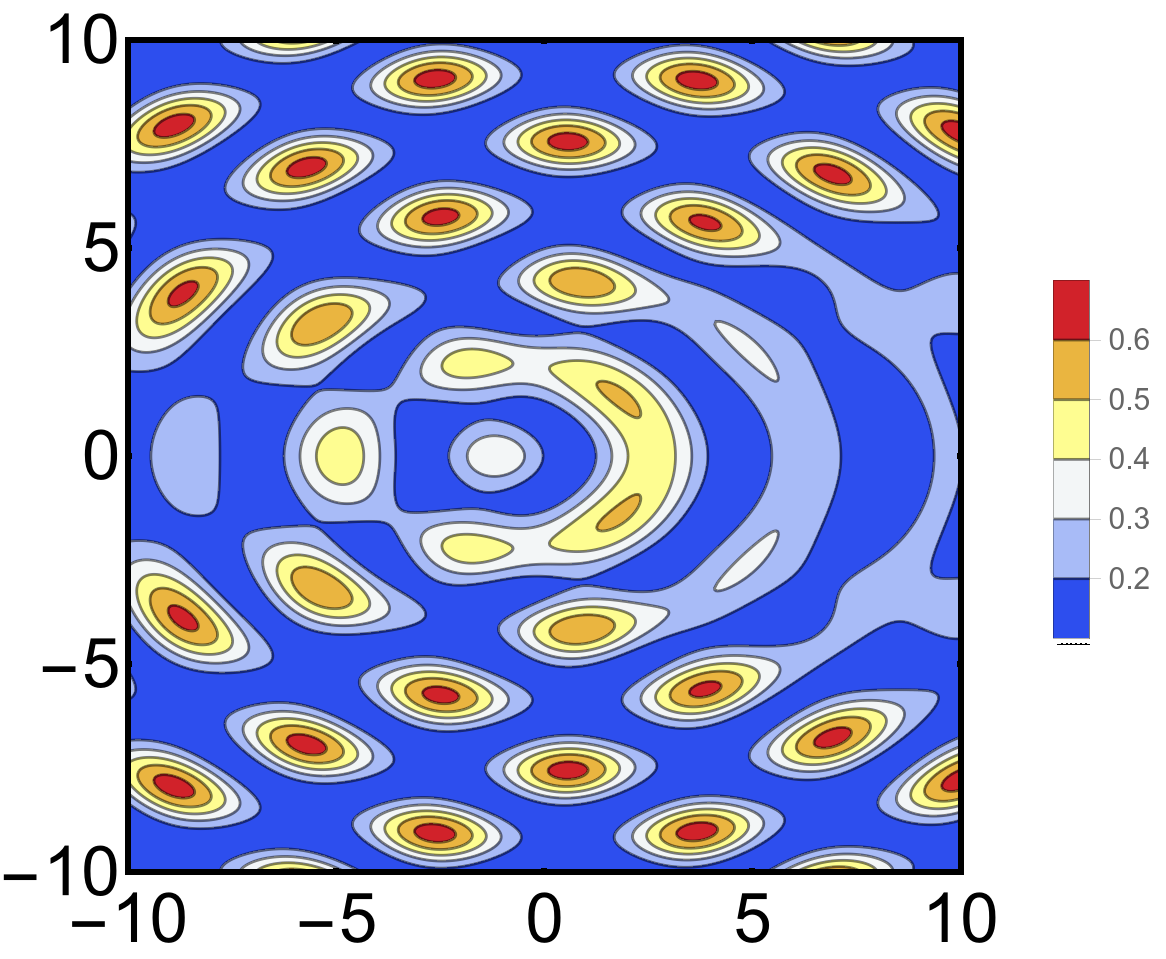
\includegraphics[width=0.6\textwidth]{Figures/gate-learning/GL_2dDensityPlot_Fredkin_Generator.png}
    \caption{
        Average gate fidelity as a function of two of the coefficients in the Hamiltonian.
        To generate this figure, we started with an ansatz for a Fredkin gate using the interactions used in~\cref{eq:GL:fredkin_generator}. We then maximised the average gate fidelity over the interaction coefficients, using random starting values. The optimiser fails to find a solution generating the Fredkin gate with good fidelity. We then used the values of the coefficients at which the optimiser stopped, fixed all except two of them --- call them $c_1$ and $c_2$ --- and plotted the average gate fidelity changing these two coefficients.
        The values of $c_1,c_2$ given by the optimiser correspond to the local maximum around the centre.
    }
    \label{fig:GL:2dDensityPlot_Fredkin_Generator}
\end{figure}

\begin{figure}[tbh]
    \centering
    \hspace{-30pt}\begin{minipage}{0.45\linewidth}
        \centering
        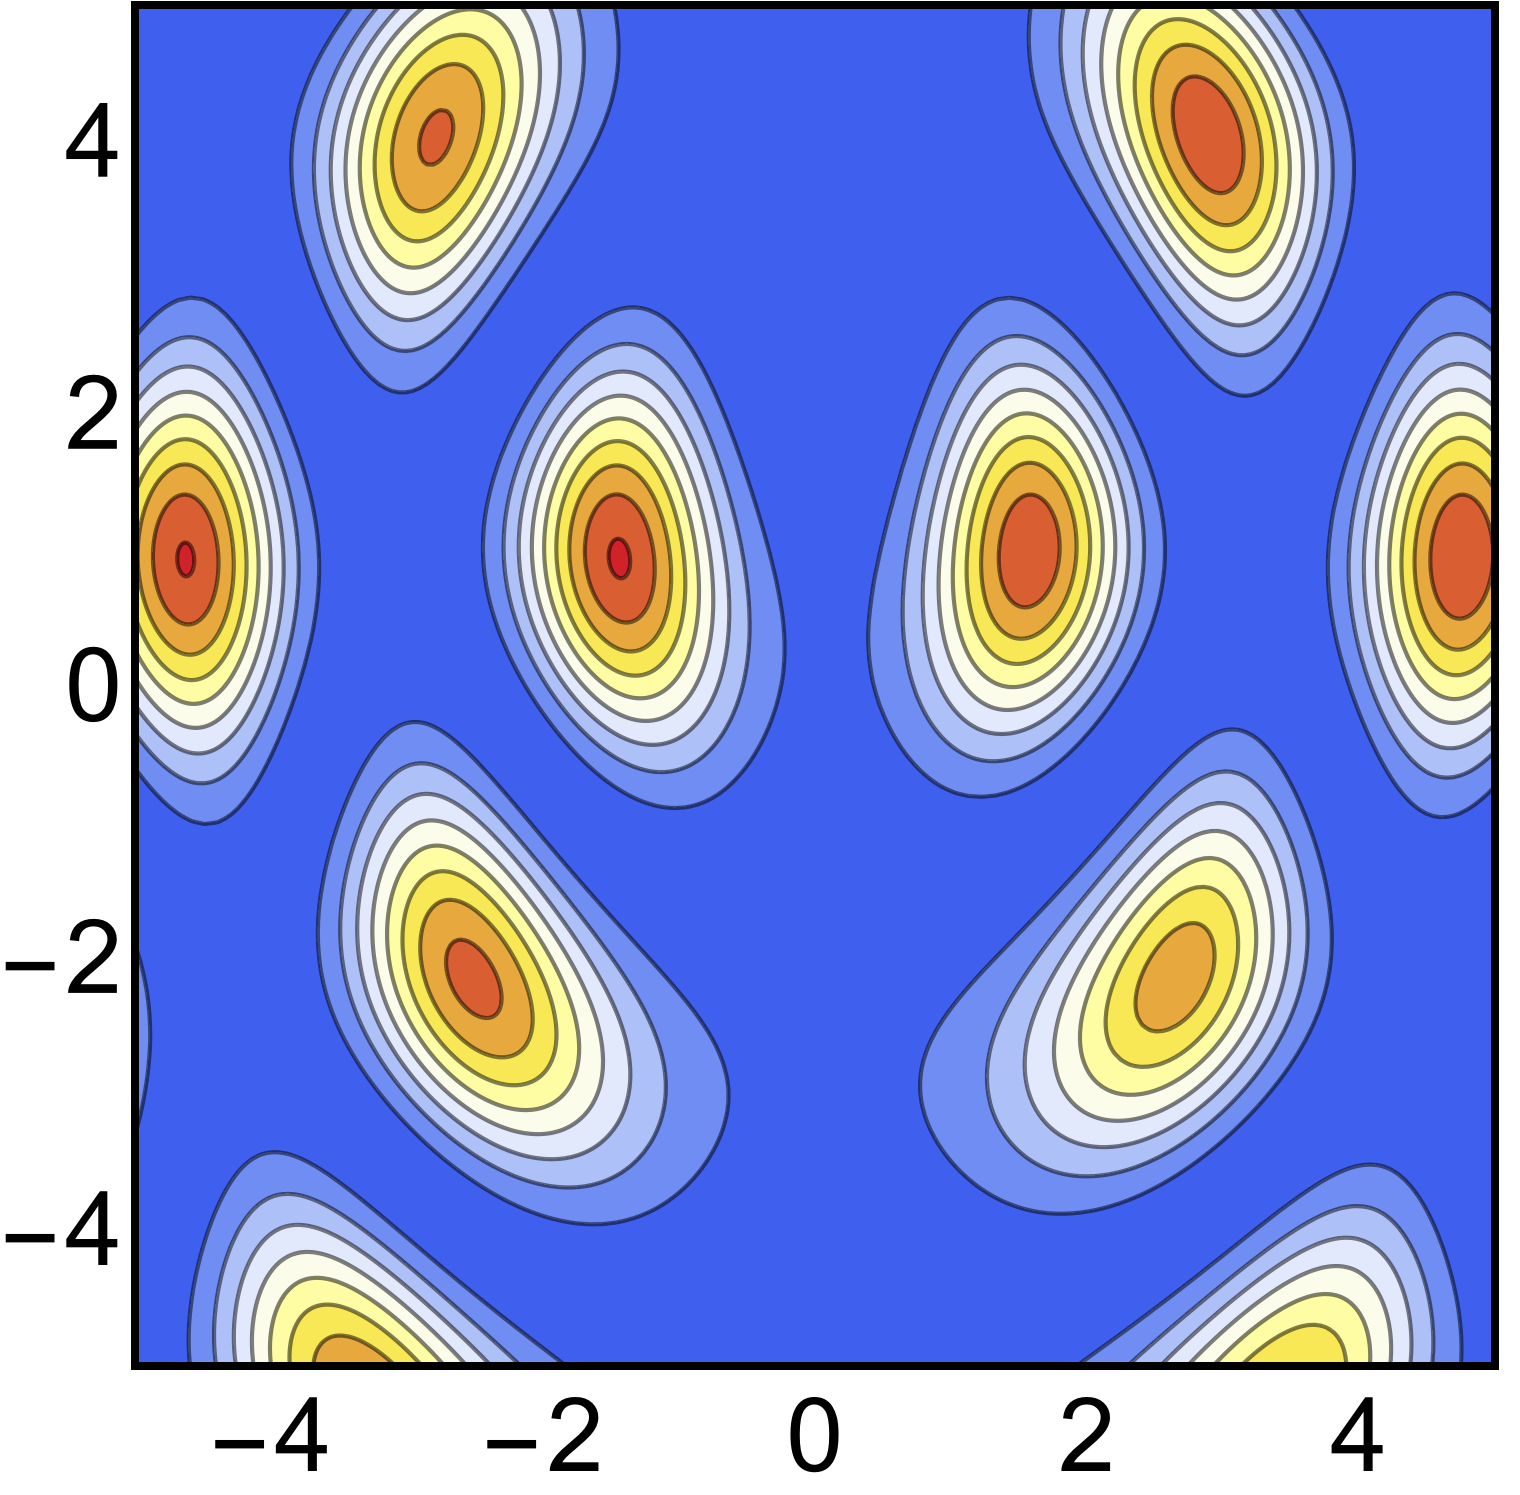
\includegraphics[height=\textwidth]{Figures/gate-learning/GL_2dDensityPlot_Toffoli_Generator.png}
    \end{minipage}\hspace{20pt}
    \begin{minipage}{0.45\linewidth}
        \centering
        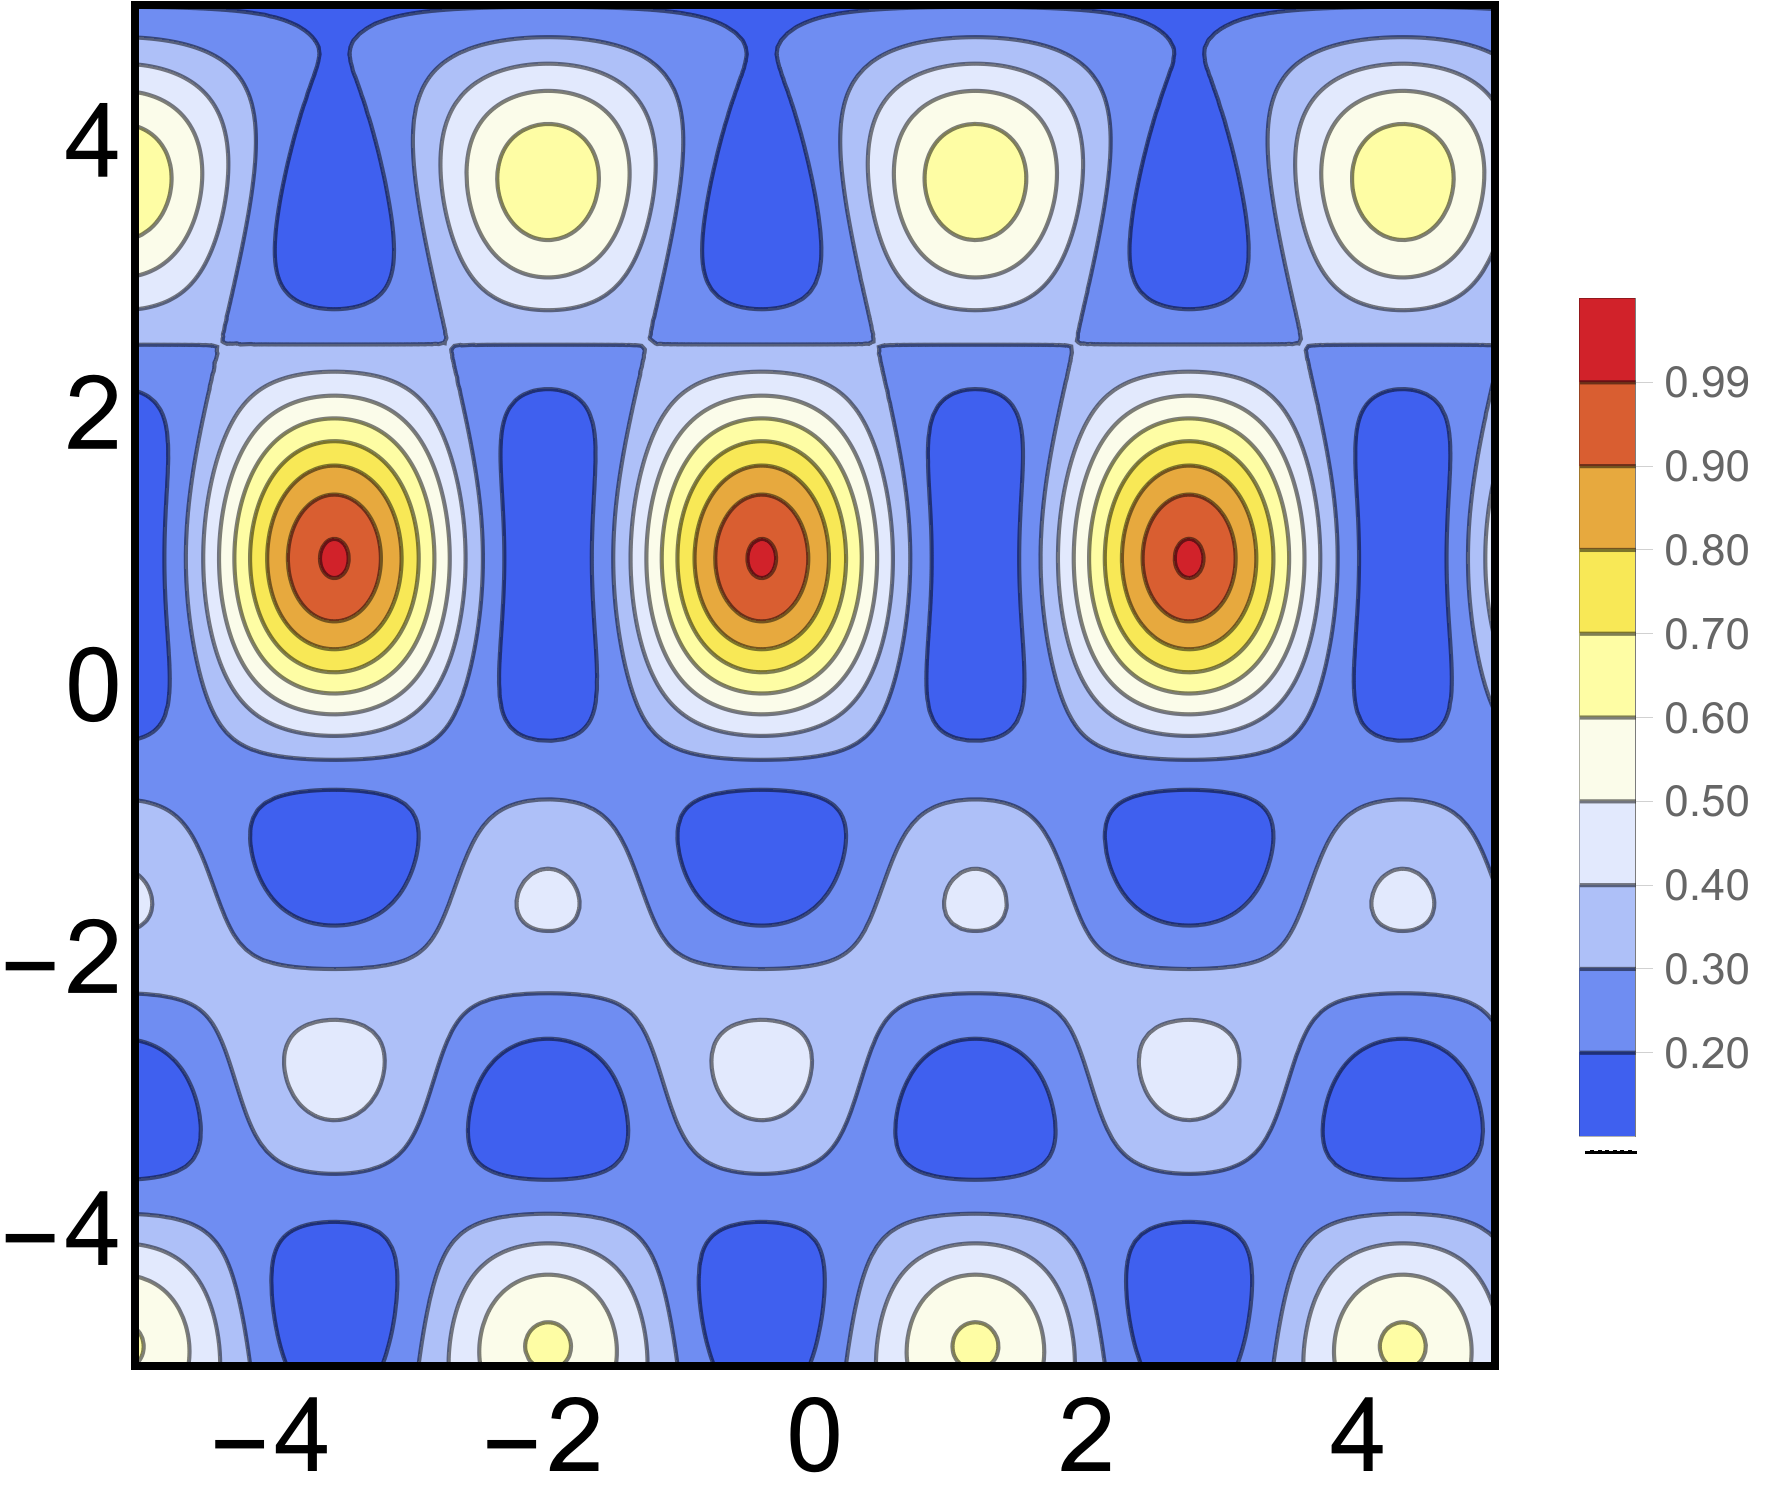
\includegraphics[height=\textwidth]{Figures/gate-learning/GL_2dDensityPlot_Toffoli_Generator2.png}
    \end{minipage}
    \caption{
        Same as~\cref{fig:GL:2dDensityPlot_Fredkin_Generator}, but using as starting ansatz a generic $\HTildeToff$ that commutes with $\UToff$ and does not use $Y$ interaction terms.
        This time, the Hamiltonian produced by the optimiser generates a Toffoli with average gate fidelity $>1- 10^{-13}$.
        We then fix all except a pair of coefficients, and plot the corresponding variations of the average gate fidelity. The two figures are obtained using two different pairs of interaction parameters from the same Hamiltonian.
        The solution given by the optimiser corresponds to the centre-left peak in the left figure, and the peak around the middle of the figure on the right.
    }
    \label{fig:GL:2dDensityPlot_Toffoli_Generator}
\end{figure}


\section{Supervised learning optimisation}
\label{sec:GL:supervised_learning}

\tmpHeading{Why does ML help?}
As discussed in~\cref{sec:GL:numerical_approach}, while the problem can be approached with standard numerical optimisation techniques, this strategy has in general limited success.
The problem lies in the mapping $\bslambda\mapsto\abs{\Tr(\calU^\dagger \calU_{\bslambda})}^2$ being not convex, which makes finding the global maximum a generally difficult task.
The technique we present here, by borrowing from ideas used in the field of supervised ML, can be used  to tackle gate design problems more efficiently, thus extending and improving on the ideas presented in~\cite{banchi2016quantum}.
In particular, the use of \ac{AD}~\cite{baydin2018automatic,bartholomewbiggs2000automatic,wengert1964a,bischof2008advances} brings dramatic improvements, efficiency-wise, thus making it possible to explore a variety of different gate learning scenarios and optimising over potentially hundreds of Hamiltonian parameters.
On top of this, the conditions given in~\cref{sec:GL:solution_framework} further speed-up the numerical training, allowing to remove unnecessary interaction parameters.

\tmpHeading{Outline of the section}
In~\cref{subsec:GL:supervised_learning_and_SGD,subsec:GL:backpropagation} we provide the necessary background on supervised learning, SGD, and AD. We then discuss in~\cref{subsec:GL:supervised_learning_for_GL} how and why supervised learning can play a part to solve gate design problems.
Then,~\cref{subsec:GL:implementation_details} contains the implementation details of the algorithm we used, and~\cref{subsec:GL:supervised_learning_results_noancillae,subsec:GL:supervised_learning_results_withancillae} present the results obtained applying this framework to a variety of target gates.

\subsection{Supervised learning and stochastic gradient descent}
\label{subsec:GL:supervised_learning_and_SGD}

\tmpHeading{Supervised learning and NNs}
Supervised learning is the task of inferring or approximating a function, given a dataset of pre-labelled data~\cite{bishop2006pattern,mohri2012foundations}.
A supervised learning algorithm starts with some \emph{model} --- a functional relation $g_{\bslambda}$ parametrised by a set of parameters $\bslambda$ --- and finds a $\bslambda_0$ making $g_{\bslambda_0}$ as close as possible to a target function $f$.
To do this, a set of pre-labelled \emph{training data} $\{ (x_1, y_1), (x_2,y_2), ...\}$ is used,
where here $y_k=f(x_k)$ is the output that we want the algorithm to associate to the input $x_k$.
An important class of supervised learning models are the so-called \acp{NN}~\cite{hechtnielsen1989theory,haykin1998neural}.
These are parametric non-linear models which play a prominent role in many machine learning tasks, such as dimensionality reduction, classification, and feature extraction.
Other contexts in which \acp{NN} have also recently proven useful include quantum many-body theory~\cite{amin2016quantum,wang2016discovering,hush2017machine,carleo2017solving,carrasquilla2017machine,torlai2017manybody,broecker2017quantum,deng2017quantum},
quantum compilation~\cite{swaddle2017generating}, quantum stabilizer codes~\cite{krastanov2017deep} and entanglement quantification~\cite{gray2018machinelearningassisted} and classification~\cite{harney2019entanglement}. We refer to~\cref{sec:intro:ML} for additional references and background.

\tmpHeading{How does SGD work?}
A \ac{NN} is \emph{trained} by optimising its parameters using a dataset of pre-labelled data.
% A common such method is the so-called \ac{SGD}~\cite{bishop2006pattern}.
A common way to do this is using a variation of a technique called \acf{SGD}~\cite{wengert1964a,ruder2016overview}.
Gradient-descent-based algorithms seek to maximise a given cost function $f(\bs x)$ by iteratively changing $\bs x$ in the direction of maximum increase of $f$, via the updating rule $\bs x\mapsto\bs x-\eta\grad f(\bs x)$.
The parameter $\eta$ is, in this context, commonly referred to as the \emph{learning rate}.
% Starting from an initial point $\bs x_0$, a number of small steps following the direction of maximum slope, $\grad f(\bs x)$, allow to follow the local gradient and thus reach a local maximum/minimum of the function.
\emph{Stochastic} gradient descent is, on the other hand, used when the goal is to optimise over \emph{functional relations}. In other words, rather then trying to minimise a cost function with a single variable $f(\bsx)$, the goal is now to minimise a function $f(\bsx,\bs w)$ with respect to its second input $\bs w$, for each value of $\bs x$.
The prototypical context in which this situation arises is when $\bs w$ are parameters representing a functional relationship $f_{\bs w}$, for example the coefficients defining a certain state of a \ac{NN}.
% \ac{SGD}, on the other hand, is suitable for a situation in which one is given a parametrised functional relationship of the form $f(\bs x; \bs w)$, and asked for a set of ``parameters'' $\bs w_0$ such that $f(\bs x; \bs w_0)$ is minimum (maximum) for all \emph{inputs} $\bs x$.
Such a case can be handled via \ac{SGD}, which in its simplest form involves starting with a random $\bs x_1$, executing a number of gradient descent iterations over $\bs w$, then picking a new $\bs x_2$ and iterating the procedure.
This corresponds to an updating rule of the form
\begin{equation}
	\bs w \to \bs w - \eta\grad_{\bs w}f(\bs x;\bs w).
	\label{eq:GL:updating_rule}
\end{equation}
While standard gradient descent, being a local optimisation algorithm, is liable to getting stuck into local minima, \ac{SGD} is generally more robust.
A core observation is that, for every input $\bsx$, one has a different parameter landscape $\bsw\mapsto f_\bsw(\bsx)$ over which the gradient descent is performed.
This new parameter landscape does \emph{not in general have the same local minima as the previous ones, whereas the global minimum is bound to be a minimum for all $\bsx$}.
In the qubit network scenario that we are tackling, this translates into the fidelity being unital for all $\ket\psi$ only for $\bslambda$ such that $\exp(i\calH_\bslambda)=\calU$.
Many variations of \ac{SGD} are used in different circumstances.
For example, in the so-called \emph{mini-batch} \ac{SGD}, instead of updating with a single input $\bs x$, one uses a \emph{batch} of inputs $\{\bs x_1,...,\bs x_M\}$, and updates the parameters using the averaged gradient:
$\bs w\to\bs w-\eta\sum_{k=1}^M\grad_{\bs w}f(\bs x_k; \bs w)/M$.
More sophisticated updating rules are used to increase the training efficiency in different circumstances.
Common techniques involve dynamically updating the learning rate, or using \emph{momentum gradient descent}~\cite{goh2017momentum,ruder2016overview}.

\tmpHeading{How is gate design a supervised learning problem?}
To see how this class of optimisation algorithms is relevant to gate design problems, consider the fidelity function $\calF$ defined as
\begin{equation}
	\calF_\bslambda(\psi) \equiv \mel{\psi}{\calU^\dagger \exp(i \calH_\bslambda)}{\psi},
	\label{eq:GL:def_fidelity}
\end{equation}
with $\calU$ the target gate, $\bslambda$ the set of parameters, and $\psi\equiv\ket\psi$ an input state.
The gate design problem is then equivalent to finding $\bslambda$ such that $\calF_\bslambda(\psi)$ is maximised (that is, equal to 1) for all $\psi$.
One possibility is to consider the average fidelity $\barcalF(\bslambda)$, as in~\cref{sec:GL:numerical_approach}, and look for its maximum using standard optimisation methods, such as standard gradient descent or differential evolution~\cite{chakraborty2008advances}.
This however, as discussed in~\cref{sec:GL:numerical_approach}, reveals to be often impractical, due to the complexity of the associated parameter landscapes.
On the other hand, \ac{SGD} allows to apply a simple and efficient local maximisation method, being at the same time less prone to getting stuck into local maxima.
This works particularly well for our problem, because we know that the $\bslambda$ corresponding to the target gate are \emph{all and only} those such that \emph{for all inputs $\psi$} the fidelity equals $1$.
Indeed, one of the main advantages of this method is its focusing on optimising $\bslambda$ for many fixed states $\psi$, rather than attempting to optimise directly the operator like we did in~\cref{sec:GL:numerical_approach}.
This is because we know that \emph{for every $\psi$}, the function $\bslambda\mapsto \calF_\bslambda(\psi)$ has a maximum some value of the parameters $\bslambda=\bslambda_0$ (at least when the gate can be implemented with the given restrictions). However, for any other $\bslambda$, changing $\psi$ changes the value of the fidelity. The consequence is that local maxima, which are problematic for optimisation algorithms, will in general disappear when the state $\psi$ is changed during the optimisation, thus making it harder for the optimiser to get stuck into local maxima.

\tmpHeading{Computing the gradients efficiently}
A critical step in gradient descent algorithms, efficiency-wise, is the evaluation of the gradient.
Numerically approximating the gradient, as done in previous works~\cite{banchi2016quantum}, is generally inefficient and scales badly with the number of optimised parameters.
An alternative to numerical differentiation is \emph{symbolic differentiation}: computing the expressions for the derivatives analytically and then hard-code the corresponding expressions into the algorithm. This can give significant improvements over numerical differentiation, but comes with its own set of problems: deriving these expressions manually would make the algorithm less flexible and requiring to be changed for each different cost function; moreover, even if a computer algebra system were used to automatically compute these expressions, there is no guarantee of getting simple or efficient expressions in general, as the derivatives can get very convoluted for complex functions.
Here we will instead make use of \acf{AD}~\cite{bartholomewbiggs2000automatic,bischof2008advances,baydin2018automatic}.
\ac{AD} improves significantly the training efficiency, allowing to explore a richer variety of scenarios.

% Another recent application of a machine learning technique to a quantum control problem,
% to find interactions implementing various 3-qubit gates like Toffoli and Fredkin,
% has been reported in~\cite{zahedinejad2015highfidelity,zahedinejad2015designing}.
% In these works however the context is completely different than ours,
% as they aim to use time-dependent interactions to implement the desired evolution,
% while we rely on the unmodulated dynamics of a network with fixed interactions.


\subsection{Automatic differentiation and backpropagation}
\label{subsec:GL:backpropagation}

\tmpHeading{Efficiency of computing the gradients}
The gradient evaluation phase is, efficiency-wise, crucial in the training of a NN.
% In fact, large networks contain many weight parameters $w_k$, and the computation of the gradient $\grad E(\bs w^{(t)})$ requires the computation of $\partial_{w_k} E(\bs w^{(t)})$ for all such $k$.
Computing the partial derivatives of the cost function with a standard numerical method, like finite differences, has a complexity $\mathcal O(N_{\bs w}^3)$, with $N_{\bs w}$ the number of parameters to differentiate~\cite{bishop2006pattern}.
This inefficiency can however be avoided using \emph{error backpropagation} via \acf{AD}~\cite{baydin2018automatic,bartholomewbiggs2000automatic,wengert1964a,bischof2008advances}.
With this technique, the complexity of the gradient evaluation phase can be cut down to $\mathcal O(N_{\bs w}^2)$~\cite{bishop2006pattern}.
This works by first decomposing the cost function in terms of elementary operations, that is, functions the gradient of which is known analytically.
In this way we build a \emph{computational graph}: a directed graph representing the functional relation between input and output as a sequence of elementary operations applied iteratively.
A computational graph is a directed acyclic graph, whose nodes represent the operations, and edges the flowing direction of inputs into outputs (see~\cref{fig:automatic-differentiation}).
Once the computational graph is built, the derivatives with respect to the model parameters can be computed efficiently.
This happens in two stages, as schematically illustrated in~\cref{fig:automatic-differentiation}.
At first, every node of the computational graph is progressively evaluated, starting from the inputs (the current values of the model parameters) up to the final value of the cost function.
During this process, the intermediate values of the elementary operations are cached (that is, stored in memory for later use).
This is the so-called \emph{feed-forward} phase.
The second phase, the so-called \emph{backpropagation} phase, starts from the output, and consists of progressively evaluating the gradients of the cost function with respect to the independent variables.
The gradient of the cost function can then be computed easily from these quantities, thanks to the chain rule of differentiation.

% The core mechanism behind backpropagation is the chain rule of differentiation.
% The name refers to the fact that, exploiting the chain rule of differentiation, the gradient of a complicated function can be expressed in a way that is recursively computed by traversing the neural network in the reverse direction.
% More specifically, when using error backpropagation in reverse-accumulation mode the gradient evaluation is comprised of two steps:
% 1) Given an input vector $\bs x$, forward propagate it through the network, finding and memorizing the activations of all hidden and output neurons, and
% 2) Now starting from the outputs and going back towards the inputs, use the chain rule of differentiation to compute the gradient of the output function $E(\bs w)$ with respect to all inputs $\bs x$.
\tmpHeading{An example to understand better}
To better understand \ac{AD}, let us work out a simple example.
Suppose the cost function is of the form
$F(\bs x)\equiv f(\bs g(\bs h(\bs x)))$.
Here, $\bs x$ is the vector of input parameters, and $f,\bs g,\bs h$ are the intermediate ``elementary'' functions, the gradients of which are assumed to be known analytically.
Using the chain rule, the gradient of $F$ then reads
\begin{equation}
    \partial_i F = \sum_{j,k}
        (\partial_j f)(\bs y^{(2)}) \cdot
        (\partial_k g_j)(\bs y^{(1)}) \cdot
        (\partial_i h_k)(\bs x),
\end{equation}
where $\bs y^{(1)}\equiv\bs h(\bs x)$ and $\bs y^{(2)}\equiv \bs g(\bs h(\bs x))$.
Remember that, in this expression, the expressions for the partial derivatives, $\partial_j f,\partial_k g_j, \partial_i h_k$, are assumed to be known beforehand.
During the \emph{feed-forward phase} the values of $\bs y^{(1)}$ and then $\bs y^{(2)}$ are progressively computed and cached from the value of $\bs x$.
The values of $\partial_i F$ can then be computed.
This method allows to efficiently evaluate numerically the gradient of arbitrary functions, without resorting to numerical approximations.

\tmpHeading{Differentiating algorithms?}
Note how arbitrary functions can be written iteratively, like $F$ here, being every computation eventually reduced to a series of elementary operations applied sequentially.
Overall, this procedure can thus be used to ``\emph{compute the derivative of an algorithm}''. By this, we mean that this procedure can be automatised into an algorithm which, given another algorithm which takes real numbers as inputs and outputs, produces an algorithm which computes the partial derivatives for each numeric input.
This is what is often used in practice to compute the gradients when SGD is used, for example in the context of NNs. Open source frameworks of widespread use that implement this functionality include Theano~\cite{team2016theano}, PyTorch~\cite{paszke2017automatic}, TensorFlow~\cite{tensorflow2015-whitepaper}.

\tmpHeading{How is this used in the context of NNs?}
In the context of training NNs, the function to be derived is the \emph{cost function} of the network, that is, roughly speaking, the (euclidean) distance between the result obtained for an input and the corresponding training output.
For the gate design problem, we will use another notion of \emph{distance} between output obtained and output expected.
For quantum states, the fidelity between these turns out to work well.

\begin{figure}[tb]
	\centering
	\begin{minipage}{0.3\linewidth}
		\centering
		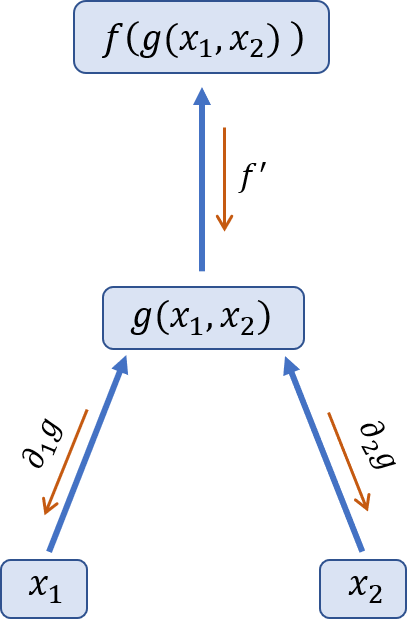
\includegraphics[height=1.3\textwidth]{automatic-differentiation}
	\end{minipage}\hfill
	\begin{minipage}{0.3\linewidth}
		\centering
		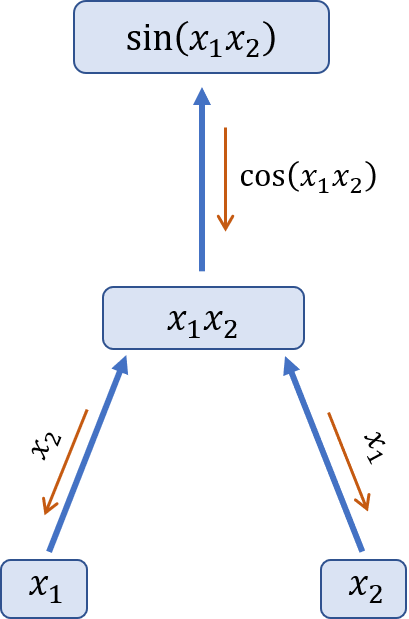
\includegraphics[height=1.3\textwidth]{automatic-differentiation2}
	\end{minipage}\hfill
	\begin{minipage}{0.3\linewidth}
		\centering
		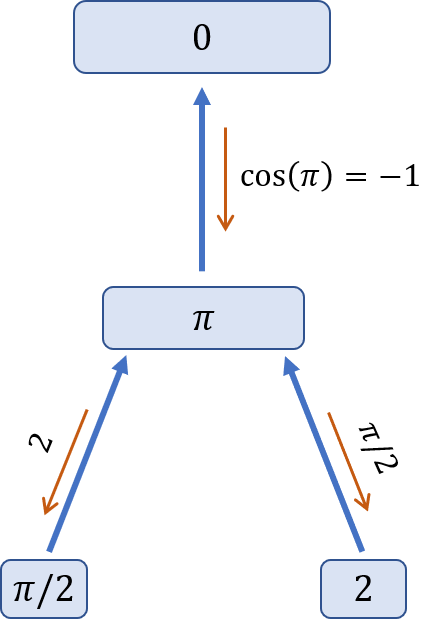
\includegraphics[height=1.3\textwidth]{automatic-differentiation3}
	\end{minipage}
	\caption{
		Examples of \ac{AD} in backpropagation mode.
		\textbf{(a)}
		Schematic representation of \ac{AD} of a function with one output and two inputs.
		Starting from numerical values for $x_1$ and $x_2$, one computes $g(x_1, x_2)$ and then $f(g(x_1, x_2))$.
		To get $\grad f(g(x_1, x_2))$, one then computes $f'(g(x_1, x_2))\partial_i g(x_1, x_2)$.
		Note that all components of this expression are known: $f'$ and $\partial_i g$ are known by assumption, and the value of $g(x_1, x_2)$ has been computed and cached in the forward propagation phase.
		\textbf{(b)} Example of application of \ac{AD} to compute the gradient of $\cos(x_1 x_2)$.
		\textbf{(c)} Using the same example function as (b), we give an example of the actual number computed at all stages when the inputs are $(x_1, x_2) = (\pi / 2, 2)$.
	}
	\label{fig:automatic-differentiation}
\end{figure}

\subsection{Supervised learning for gate design problems}
\label{subsec:GL:supervised_learning_for_GL}

\tmpHeading{Don't throw the baby out with the bathwater}
The main idea is to merge supervised learning techniques with the analytical results derived in~\cref{sec:GL:solution_framework}.
What made finding generators difficult, in~\cref{sec:GL:toffoli,sec:GL:fredkin} was imposing the condition on the eigenvalues given in~\cref{sec:GL:solution_framework}, whereas the commutativity condition,~\cref{eq:GL:3conditions_2nd}, is generally straightforward to impose, amounting to a series of linear equations.
What we can do is then to keep the latter condition, and use it as a starting point for the numerical optimisation, thus avoiding having to deal directly with the hard eigenvalue problem.

\tmpHeading{The plan}
For the purpose, we consider a slight generalisation of the gate learning problems discussed previously in the chapter. Each gate learning problem is defined by a target gate $\calU$, and a set of available interactions $\calP\equiv \{\sigma_i\}_i$, so that the ansatz generator has the form $\calH_\bslambda=\sum_i \lambda_i \sigma_i$. As in~\cref{sec:GL:solution_framework}, we use the commutativity condition $[\calH_\bslambda,\calU]=0$ to cut down the number of free parameters. However, rather than trying to tackle the eigenvalue condition, we now instead feed the reduced expression for $\calH_\bslambda$ directly into the supervised learning optimisation algorithm. The algorithm will then look for values of $\bslambda$ which maximise the fidelity $\calF_\bslambda(\psi)\equiv\mel{\psi}{\calU^\dagger \exp[i\calH_\bslambda]}{\psi}$ for all input states $\psi\equiv\ket\psi$.
AD makes this easier by making the evaluation of the derivatives $\partial_{\lambda_i}\calF_\bslambda(\psi)$ efficient.

\tmpHeading{We can add ancillary qubits without changing the algorithm}
This allows to also easily consider more general cases than those analysed analytically in the previous sections. In particular, we can consider scenarios with ancillary qubits without changing much in the optimisation algorithm.
This scenario is similar to what was considered in~\cite{banchi2016quantum}.
We think of the $n$-qubit system as partitioned into $n_S$ \emph{system qubits} and $n_A$ \emph{ancillary qubits}. The goal will be to use the ancillary qubits to implement a target evolution on the system ones. More precisely, fixed an initial state $\ket\phi$ for the ancillae and an initial system state $\ket\psi$, we evolve the input through the given Hamiltonian and trace out the ancillae at the end:
\begin{equation}
    \rho_{\on{out}}^S(\bslambda) \equiv \Tr_{\on{anc}}[e^{i\calH_\bslambda}(\rho_S\otimes\rho_A)e^{-i\calH_\bslambda}],
\end{equation}
where we used the notation $\rho_S\equiv\PP[\ket\psi]$ and $\rho_A\equiv\PP[\ket\phi]$ to denote the projectors corresponding to the states. This output state is then compared with the (pure) target state, $\psi_{\on{target}}\equiv\calU\ket\psi$. The final fidelity used to evaluate the quality of the network at each iteration is then
\begin{equation}
    \calF_\bslambda(\psi) = \mel{\psi_{\on{target}}}{\rho^S_{\on{out}}(\bslambda)}{\psi_{\on{target}}}.
    \label{eq:GL:fidelity_map_vs_unitary}
\end{equation}
It is worth noting that, in practice, the only thing that needs to be changed in the algorithm to handle this new scenario with ancillae is this fidelity function (and of course the Hamiltonian ansatz).
Because the results about commutativity found in~\cref{sec:GL:solution_framework} assume a fully unitary evolution (which is here broken by the partial trace operation), they cannot be used to improve the ansatz in the case with ancillae.

\tmpHeading{Interaction terms used for the optimisations}
We focus on the scenario in which only one- and two-qubit interactions are available. The initial Hamiltonian ansatz (before further commutativity conditions are considered) thus has the form
\begin{equation}
    \calH_\bslambda = h_0 I + \sum h^\alpha_{i} \sigma_i^\alpha + \sum J_{ij}^{\alpha\beta} \sigma_i^\alpha \sigma_j^\beta.
    \label{eq:GL:hamiltonian_atmostpairwise}
\end{equation}
Here, $i, j=1,...,N$ index the qubits comprising the system, $\alpha, \beta\in\{1,2,3\}$ identify the considered Pauli matrices (we use the correspondence $\sigma^1\rightarrow\sigma^x, \sigma^2\rightarrow\sigma^y, \sigma^3\rightarrow\sigma^z$), $J_{ij}^{\alpha\beta}$ are the coupling strengths, and $\bslambda\equiv \{h_0, h^\alpha_{i}, J_{ij}^{\alpha\beta}\}$.
Note that, for a given choice of $\calU$ and $\calH_\bslambda$, it is not known a priori whether a solution to the gate learning problem exists, although it is easy to check whether a proposed solution satisfies the criterion.
% For example, it was until recently assumed that nontrivial three-qubit gates such as Toffoli and Fredkin could not be implemented with a time-independent dynamics without making use of ancillary qubits or higher-dimensional spaces~\cite{banchi2016quantum,zahedinejad2015highfidelity,zahedinejad2015highfidelity} (check).
Indeed, a simple parameter-counting argument shows it does not in general: not all possible evolutions produced using higher-order interactions can be generated when only one- and two-qubit couplings are available.
% A concrete example of the gate-synthesis problem discussed here is given by the implementation of a Toffoli gate~\cite{shi2002both} over a three-qubit network with a restricted set of interactions. Yet,~\cite{banchi2016quantum} showed that the use of a single ancillary qubit catalyses the synthesis of three-qubit gates with the restricted resources mentioned above. We found, however, that the same task can be achieved \emph{without} ancillary qubits and under the stronger restriction of having available only \emph{diagonal} pairwise interactions. Whether a given gate can be realised with a specific time-independent set of interactions remains an open question.


\subsection{Implementation details}
\label{subsec:GL:implementation_details}

\tmpHeading{What tools did we use?}
We used Python as the language of choice to implement the supervised-learning-based optimisation.
Being Python language of widespread use in the machine learning community, many libraries and frameworks are available to build computational graphs over which \ac{AD} can be used.
In particular, we used \textsc{Theano}~\cite{team2016theano}, together with the \textsc{QuTiP} library to handle some of the operations involving quantum states~\cite{johansson2012qutip,johansson2013qutip}.
% The code used, together with a number of usage examples, is available on GitHub (\href{https://github.com/lucainnocenti/quantum-gate-learning}{Link}).

\tmpHeading{What is the goal of the algorithm?}
The goal of the algorithm is, given a target gate $\mathcal G$ and an ansatz $\bslambda\mapsto\calH_\bslambda$ for the Hamiltonian, to find the $\bslambda_0$ such that $\exp(i\calH(\bslambda_0))=\calG$.
We employ for the purpose \emph{mini-batch momentum \ac{SGD}}.
The \emph{mini-batch} version of \ac{SGD} involves computing the gradient, at every iteration, averaging over the gradients computed for a number of states.
In other words, the training dataset is partitioned into a series of \emph{mini-batches}, and to evaluate the size and direction of the step on the parameters, the gradient is computed by averaging over the gradients computed for each element of the mini-batch.
Varying the size of such batches can be used to tune the variance of the gradients with respect to the input states.
The use of \emph{momentum}~\cite{ruder2016overview,goh2017momentum} involves using a modified version of the updating rule given in~\cref{eq:GL:updating_rule}, which becomes
\begin{equation}
\begin{aligned}
    \bs v &\to \gamma \bs v + \eta \grad_{\bslambda} \calF_\bslambda(\psi), \\
    \bslambda &\to \bslambda + \bs v,
\end{aligned}
\label{eq:GL:updating_rule_momentum}
\end{equation}
where $\gamma$ is often referred to as the \emph{momentum} parameter.
Using the auxiliary parameter $\bs v$ during the training discourages sudden changes of direction in the evolving parameter, and thus usually makes the training significantly more robust~\cite{goh2017momentum}.

\tmpHeading{Scope of the algorithm}
Our implementation allows to train arbitrary target gates parametrised via a time-independent Hamiltonian $\calH_\bslambda$.
Any $\calH_\bslambda$ depending linearly on the parameters, $\calH_\bslambda=\sum_i \lambda_i \sigma_i$ for Hermitians $\sigma_i$, can be used.
This is made possible by the flexibility of \ac{AD}, which allows to automatically build an efficiently differentiable computational graph, without needing to hard-code the structure of the Hamiltonian and its derivatives with respect to $\lambda_i$.

\tmpHeading{Handling complex numbers}
While the cost function $\calF$ is always real, some of the intermediate calculations needed to compute it involve complex numbers.
While this poses no fundamental problems, many of the \ac{ML} libraries do not support \ac{AD} over functions with complex inputs or outputs.
We worked around this problem using a similar trick to the one reported in~\cite{leung2017speedup}.
In particular, to use the existing framework, we mapped the problem into one involving only real numbers.
To do this, we map complex matrices into real ones via the bijection
$A\mapsto\mathfrak{Re}(A)\equiv I \otimes A_{R} - i \sigma_y\otimes A_{I}$,
where $A_R$ and $A_I$ are the real and imaginary parts of $A$, respectively.
At the same time, state vectors are to be mapped to
$\Psi\mapsto\mathfrak{Re}(\Psi)\equiv(\Psi_R, \Psi_I)^T$.
It is easy to verify that with this mapping
$A\Psi\mapsto\mathfrak{Re}(A\Psi)=\mathfrak{Re}(A)\mathfrak{Re}(\Psi)$,
so that all calculations can be equivalently be carried out with the real versions of matrices and vectors.

\tmpHeading{Step-by-step description of the algorithm}
More specifically, the algorithm involves the following steps:
\begin{enumerate}
	\item Choose an initial set of parameters $\bslambda$ (randomly, or specific values if one has an idea of where a solution might be).
	A number of other hyperparameters have to be decided at this step, depending on the exact \ac{SGD} method used. In particular, for mini-batch \ac{SGD} with momentum and decreasing learning rate, one has to decide the momentum $\gamma$, the initial value of $\eta$, the rate at which $\eta$ decreases during the training, and the size $N_b$ of the batches of states used for every gradient descent step.
	\item Repeat the following loop $N_e$ times, or until a satisfactory result is obtained.
	Each such iteration is conventionally named an \emph{epoch}.
	Another hyperparameter to be chosen beforehand is the number of training states $N_{tr}$ to be used in each epoch.
	Once this is fixed, every epoch will involve a number $N_{tr}/N_e$ of gradient descent steps, each one using $N_e$ states for a single gradient calculation.
	$N_e$ random training states are sampled, to be used during the epoch.
	\begin{enumerate}
		\item Pick $N_b$ of the $N_e$ training states.
		\item Forward-propagate each state of the sample, and then backpropagate the gradients, thus computing the average gradient over the mini-batch $\grad_{\bslambda} \calF(\bslambda)$.
		\item Update the coupling strengths $\lambda$ as per~\cref{eq:GL:updating_rule_momentum}.
		\item Return to point (a).
	\end{enumerate}
\end{enumerate}


\subsection{Results for unitary networks}
\label{subsec:GL:supervised_learning_results_noancillae}

\tmpHeading{Target gates used}
We test our algorithm to train generators for Toffoli, Fredkin, and \emph{double-Fredkin} gates.
Toffoli and Fredkin gates were defined and discussed in~\cref{sec:GL:toffoli,sec:GL:fredkin}.
The ``double-Fredkin'' gate is a \emph{four}-qubit gate which, conditionally on the state of the first qubit, acts either like a Fredkin, or like a Fredkin with reversed control. More explicitly, this is the gate
\begin{equation}
    \calU_{\on{FF}} \equiv \PP_0\otimes \UFred + \PP_1\otimes \calU_{\overline{\on{Fred}}},
    \quad\text{ where }\quad
    \calU_{\overline{\on{Fred}}} \equiv \PP_0\otimes \on{SWAP} + \PP_1\otimes I.
\end{equation}

\tmpHeading{Ansatzes used}
In all cases, we used an ansatz containing only one-qubit and \emph{diagonal} two-qubit interactions, that is, two-qubit interactions of the form $\sigma_i^\alpha\sigma_j^\alpha$.
For the Toffoli gate, imposing the commutativity condition on such an ansatz gives the following expression:
\begin{equation}
\begin{aligned}
    \calH_\bslambda^{\on{Toff}} &=
    h_1^z Z_1 + h_2^z Z_2 + h_3^x X_3 +
    J_{13}^{xx} X_1(1+X_3) +
    J_{23}^{xx} X_2(1+X_3) \\
    &+ J_{12}^{zz} Z_1 Z_2 +
    J_{13}^{zz} (1+Z_1)Z_3 +
    J_{23}^{zz} (Z_2 - Z_1)Z_3 +
    J_{12}^{xx} (X_1 X_2 + Y_1 Y_2).
\end{aligned}
\label{eq:GL:toffoli_reducd_ansatz_for_ML}
\end{equation}
Similar reasoning applied to the Fredkin gate gives the expression:
\begin{equation}
\begin{aligned}
    \calH_\bslambda^{\on{Fred}} &=
    (h_3^x + J_{13}^{xx} X_1) (X_2 + X_3)
    + (h_3^y + J_{13}^{yy} Y_1) (Y_2 + Y_3) \\
    &+ J_{23}^{xx} X_2 X_3
    + J_{23}^{yy} Y_2 Y_3
    + J_{23}^{zz} Z_2 Z_3
    + h_1^z Z_1
    \\
    &+ h_2^z (1 + Z_1) Z_2
    + J_{13}^{zz} Z_1 (Z_2 + Z_3)
    + h_3^z (Z_3 - Z_1 Z_2).
\end{aligned}
\end{equation}
% \begin{equation}
% \begin{aligned}
%     \calH_\bslambda^{\on{Fred}} &=
%     J_{23}^{xx} X_2 X_3 +
%     h_3^x (X_2 + X_3) +
%     J_{13}^{xx} X_1(X_2 + X_3) +
%     J_{23}^{yy} Y_2 Y_3 +
%     h_3^y (Y_2 + Y_3) \\
%     &+ J_{13}^{yy} Y_1 (Y_2 + Y_3)
%     + h_1^z Z_1
%     + h_2^z (1 + Z_1) Z_2
%     + J_{23}^{zz} Z_2 Z_3
%     + J_{13}^{zz} Z_1 (Z_2 + Z_3)
%     + h_3^z (Z_3 - Z_1 Z_2)
% \end{aligned}
% \end{equation}

% oneQubitAndDiagonalTwoQubitIntsIndices = 
%   Select[Tuples[Range[0, 3], {3}],
%    Map[Last]@Tally@DeleteCases[0]@# == {2} || 
%      Length@DeleteCases[0]@# <= 1 &
%    ];
% pauliProduct[indices__] := 
%   KroneckerProduct @@ (PauliMatrix /@ {indices});
% generalGeneratorHam = (c @@ # pauliProduct @@ #) & /@ 
%     oneQubitAndDiagonalTwoQubitIntsIndices // Total;
% generalGeneratorHam /. With[
%       {commutatorElements = #1.#2 - #2.#1 &[
%            Toffoli[], generalGeneratorHam
%            ] // Flatten // Simplify},
%       Solve[
%        Thread[commutatorElements == 0],
%        DeleteDuplicates@Cases[generalGeneratorHam, c[__], Infinity]
%        ]
%       ][[1]] // PauliBasis // QPauliExprToRegularExpr // 
%  Collect[#, c[__], Simplify] &




\tmpHeading{Summary of the results}
A sample of training results for Toffoli, Fredkin, and ``double Fredkin'' gates are given in~\cref{fig:GL:toffoli_diagonal_solutions}.
In~\cref{fig:GL:toffoli_diagonal_parhistories} we provide the training histories of the parameters for eight different solutions for Toffoli, Fredkin and \emph{double Fredkin}, respectively.
These illustrate how quickly the networks converge for different initial values of the parameters.
In all of these cases, the target gate is obtained with unit fidelity up to numerical precision (that is, all fidelities are between $1-10^{-16}$ and $1$).
Different sets of optimisation hyperparameters are found to give acceptable solutions.
For the trainings shown in this paper we used a dynamically updated learning rate given, for the $k^{\text{th}}$ epoch, by $\eta=1/(1 + k \alpha)$ with a \emph{decay rate} of $\alpha=0.005$.
The other hyperparameters were chosen as
$\gamma=0.5$, 
$N_b = 2$, $N_{tr} = 200$.
Different initial values for the parameters were tested, but in most cases we started the training with either vanishing or random (following a normal distribution) parameters.
For the training of the four-qubit gate we found the network to converge sooner to a solution when the parameters were initialised to a positive value (often with all parameters initialised to $4$).

\tmpHeading{Results for Toffoli, Fredkin, double-Fredkin}
In~\cref{fig:toffoli_fidVSpars,fig:fredkin_fidVSpars,fig:doublefredkin_fidVSpars} we report the behaviour of the fidelity upon changes of the learnt Hamiltonian parameters, for Toffoli, Fredkin and \emph{double Fredkin} gates, respectively.
As shown in these plots, the stability of the implemented gates with respect to variations of time and interactions values greatly varies between different solutions, as well as between different parameters in the same solutions.

\tmpHeading{Results with restrictive interactions}
To assess the feasibility of nontrivial gates in more restrictive experimental scenarios, we performed a systematic analysis of the reachability of Fredkin and Toffoli gates when allowing only for single-qubit and $X_i X_j+Y_i Y_j$ two-qubit interactions, and in the less restrictive setting of allowing for all $X_i X_j$ and $Y_i Y_j$ interactions.
The results are shown in~\cref{fig:fredkin_XY,fig:fredkin_XX,fig:toffoli_XX,fig:toffoli_XY}.
For the Fredkin gate, in the more restrictive $XX$ interactions setting, the biggest fidelity obtained was $\barcalF\simeq 0.94$, while when allowing for all $XX$ and $YY$ interactions the maximum fidelity obtained was $\barcalF\simeq0.999$.
For the Toffoli gate, the maximum fidelity obtained in the $XX$ scenario was $\barcalF\simeq0.94$ as well, while when allowing for all $XX$ and $YY$ interactions the best training results corresponded to $\barcalF\simeq 0.98$.
To have more consistent results, in all the training instances shown here all the hyperparameters, except for the interaction parameters' initial values, were chosen to have the same value.
In particular, each training instance was run for $200$ epochs, each one using $200$ random quantum states as inputs, divided in batches of $2$ elements.
This choice of hyperparameters is mostly empirical, and it is possible for different values to provide better results.


\tmpHeading{What do these results tell us?}
The above provides further evidence for the flexibility of the supervised learning approach, which can produce solutions with good fidelities even in more restrictive scenarios, closer to the capabilities of state of the art experimental architectures.
Furthermore, the values of the interaction strengths for many of the presented solutions are found to be compatible with the capabilities of state of the art circuit-QED architectures with gate times of the order of tens of nanoseconds~\cite{potočnik2018studying}.

\tmpHeading{Code availability}
Additional solutions and data, as well as the code used to produce them, is available on \href{https://github.com/lucainnocenti/quantum-gate-learning-1803.07119}{GitHub}\footnote{https://github.com/lucainnocenti/quantum-gate-learning-1803.07119}.
This repository contains all the code used to reproduce the solutions presented in this paper, as well as to train arbitrary gates on arbitrary numbers of qubits.
Even more generally, arbitrary (linearly) parametrised matrices can be used as training model, allowing a high degree of flexibility.

\subsection{Results for networks with ancillae}
\label{subsec:GL:supervised_learning_results_withancillae}

\tmpHeading{Training gates with ancillae}
We also showcase the capability of the network in scenarios which include larger numbers of free parameters and up to five ancillary qubits. In particular, we consider as target gates the three-qubit \ac{QFT}, the \emph{half-adder} gate~\cite{barbosa2006quantum}, and a custom gate we will refer to as a \emph{Toffredkin gate}.
The three-qubit QFT amounts, as a matrix, to the $8\times8$ discrete Fourier transform matrix, which is the matrix with components $\on{QFT}_{jk}=\omega_8^{(j-1)(k-1)}$, where $\omega_8\equiv e^{2\pi i/2^3}$ and $i,j=1,...,8$.
The half-adder gate can be defined as the gate
\begin{equation}
    \calU_{\on{ha}} \equiv \on{CNOT}_{12}\Toff,
\end{equation}
where $\on{CNOT}_{12}$ denotes the CNOT gate between the first two qubits and $\Toff$ is the Toffoli gate.
A feature of the half-adder gate is that it acts on a logical three-qubit state $\ket{p_1,p_2,p_3}$ by sending it into the state $\ket{p_1,p_1\oplus p_2,p_3\oplus \on{carry}}$, where $\on{carry}$ equals either $0$ or $1$ depending on whether the sum $p_1+p_2$ gives a remainder (that is, on whether $p_1p_2=1$).
Finally, the Toffredkin gate is a gate which acts either as a CNOT or as a SWAP on second and third qubits, conditionally to the state of the first qubit. Explicitly, this is the gate
\begin{equation}
    \calU_{\on{TF}} \equiv \PP_0\otimes\on{CNOT}_{23} + \PP_1\otimes\on{SWAP}_{23}.
\end{equation}
For the cost function $\calF_\bslambda$ we use the expression given in~\cref{eq:GL:fidelity_map_vs_unitary}, with a general Hamiltonian model with at-most-pairwise interactions, as given in~\cref{eq:GL:hamiltonian_atmostpairwise}.
This means that, for example, to train the four-qubit networks implementing half-adder and Toffredkin, we start with a general Hamiltonian with $9$ parameters $h_i^\alpha$ for the single-qubit terms, plus $3\times9$ parameters $J_{ij}^{\alpha\beta}$ for the two-qubit interactions, amounting to a total of $36$ parameters to be trained.
The $h_0$ parameter can be left out of the training as it only amounts to an unobservable global phase. A similar calculation tells us that for the $3+5$ network used to train the \ac{QFT} gate, a total amount of $276$ parameters are trained.

\tmpHeading{Assessing the quality of the results}
To assess the quality of the results we use the averaged gate fidelity $\barcalF(\calE,\calU)$ introduced in~\cref{eq:GL:explicit_fidelity_map_unitary}.
The map $\calE$ is, in our case, the operation corresponding to the action of a unitary in the enlarged system+ancillae space, followed by tracing the ancillary qubits.
Explicitly, if $\calU_\bslambda\equiv\exp(i\calH_\bslambda)$ is a unitary acting on the full system plus ancillae space, obtained from the learning procedure, then the corresponding map is
$\calE_\bslambda(\rho) = \Tr_A[\calU_\bslambda(\rho\otimes\rho_A) \calU_\bslambda^\dagger]$,
where $\rho_A$ is the initial state of the ancillae (here always fixed to be $\ket0^{\otimes n_A}$).
This average fidelity can be written explicitly in terms of the components of the map and target unitary, as given in~\cref{eq:GL:explicit_fidelity_map_unitary}. This is the expression that will be used in the following to estimate the quality of the results.

\tmpHeading{Results for QFT, half-adder, Toffredkin}
\Cref{fig:GL:parameters_QFT_Toffredkin_halfadder} shows the sets of Hamiltonian parameters that were obtained through the training procedure, for each target gate.
\begin{itemize}
    \item (\textbf{\emph{Toffredkin}}) The Toffredkin gate was found with unit fidelity, up to numerical precision, using a single ancillary qubit. In~\cref{fig:GL:toffredkin_fidVSpars} we show how the fidelity varies with the Hamiltonian parameters. \Cref{fig:GL:toffredkin_finalmatrix} reports the final matrix over the full four-qubit network.
    \item \textbf{\emph{(QFT)}} In the case of the \ac{QFT}, we performed a series of training runs with different numbers of ancillae, using from zero to five ancillary qubits.
    We observed the best results when using $0$, $3$, and $5$ ancillae, the average fidelities being $0.987$, $0.991$, and $0.988$ respectively.
    It is important to note that due to the heuristic nature of our optimization method, better results might be achieved using different initial conditions or optimization parameters.
    In~\cref{fig:GL:qft3q+5a_fidVSpars} we present the dependence of the fidelities with respect to the parameters, for the case of $5$ ancillary qubits.
    The fact that five ancillary qubits result in a lower fidelity than the case with three is likely due to the significantly larger number of parameters involved in the optimisation, which make the training harder and more time-consuming.
    \item \textbf{\emph{(Half-adder)}} Finally, the half-adder was realised with average fidelity $\barcalF\simeq0.999997$ with a single ancillary qubit.
    Again, in~\cref{fig:GL:halfadder_fidVSpars} we report the behaviour of $\calF_\bslambda$ upon variations of $\bslambda$, and in~\cref{fig:GL:halfadder_finalmatrix} we give the final unitary gate, over the full four-qubit network, found via the optimisation.
\end{itemize}

\tmpHeading{Robustness of the results}
\Cref{fig:GL:toffredkin_fidVSpars,fig:GL:halfadder_fidVSpars,fig:GL:qft3q+5a_fidVSpars} show the relative stability of the gates with respect to changes of the Hamiltonian parameters.
In particular, for Toffredkin and \ac{QFT}, the fidelity remains above $95\%$ upon a $25\%$ variation of the evolution time.
The half-adder appears to be less stable, but this is only consequence of the larger values of its interactions, as shown in~\cref{fig:GL:parameters_QFT_Toffredkin_halfadder}(c).
Indeed, the hardness of tuning the Hamiltonian parameters with sufficient precision will vary strongly between different gates, as well as between different implementation of the same gate, and between different parameters in any given implementation.
These results provide further evidence in support of the power and flexibility of the supervised learning approach presented in~\cite{innocenti2018supervised,banchi2016quantum}, which clearly applies to the cases where ancillary degrees of freedom are exploited during the evolution.


\section{Conclusions}
\label{sec:GL:conclusions}

% We have reported on strategies for supervised-learning-assisted synthesis of multi-qubit quantum gates.
We discussed strategies to synthesise multi-qubit quantum gates with time-independent Hamiltonians and constrained interactions.
After presenting the underlying mathematical structure, we proposed a way to tackle the problem, and show that it leads to exact solutions in a few cases of interest, including generators for Toffoli and Fredkin gates using only single- and two-qubit interactions.
We then proceeded to show that our framework is useful not only to reach exact conclusions, but also as a starting point to find numerical solutions.
% The general scheme of our gate design is based on the use of a limited set of resources (such as two-qubit gates) that, in general, would not be sufficient for arbitrary gate design.
% However, the catalyst effect brought about by the use of machine learning -- specifically, stochastic gradient descent -- is sufficient to overcome the limitation of our resources and deliver high-quality complex quantum gates.
Moreover, we find that a some classes of machine-learning techniques, namely stochastic gradient descent and automatic differentiation algorithms, are well-suited to tackle the associated numerical task. We show that these techniques bring about significant improvements efficiency-wise, thus allowing to explore a wide variety of gate learning scenarios.
% By importing machine-learning techniques into the discussion, 
We demonstrated the performance of our scheme by finding novel time-independent generators for nontrivial three-qubit interactions such as Toffoli, Fredkin, and \emph{Toffredkin} gates, as well as four-qubit gates, and half-adder and Quantum Fourier Transform.
% which acts as different three-qubit gates conditionally on a fourth one.
% To further test the efficiency of our approach we addressed the significant cases of a half-adder and a \ac{QFT} circuit.
% Moreover, we have shown the flexibility of our approach by addressing a novel type of gate that puts together the paradigmatic quantum Toffoli and Fredkin gates.

Our methodology has the potential to improve the design of quantum operations,
% suitable for example to simulate network dynamics,
lowering the complexity associated with gate decompositions common in quantum information protocols.
% , and simply adopting well-known techniques of classical machine learning.
Several interesting questions are spurred by this work and remain as-of-yet unanswered. From a mathematical standpoint, general conditions to certify the achievability of a gate in a given setting would be highly desirable, and shed further light into the underlying structure of the problem.
Such a result would also further our understanding of how complex physical interactions emerge from simpler ones.
Furthermore, it would be interesting to study how the problem changes when we allow as target more general quantum maps.
Finally, our use of supervised learning to tackle gate learning problems is rather problem agnostic, and thus applicable to a variety of different scenarios. Exploring what classes of problems in quantum information would gain from a similar approach would constitute a fruitful venue for research.

% \begin{figure}[tb]
% % {\bf (a)}\hskip5cm{\bf (b)}\hskip5cm{\bf (c)}
%     \centering
%     \textbf{(a)}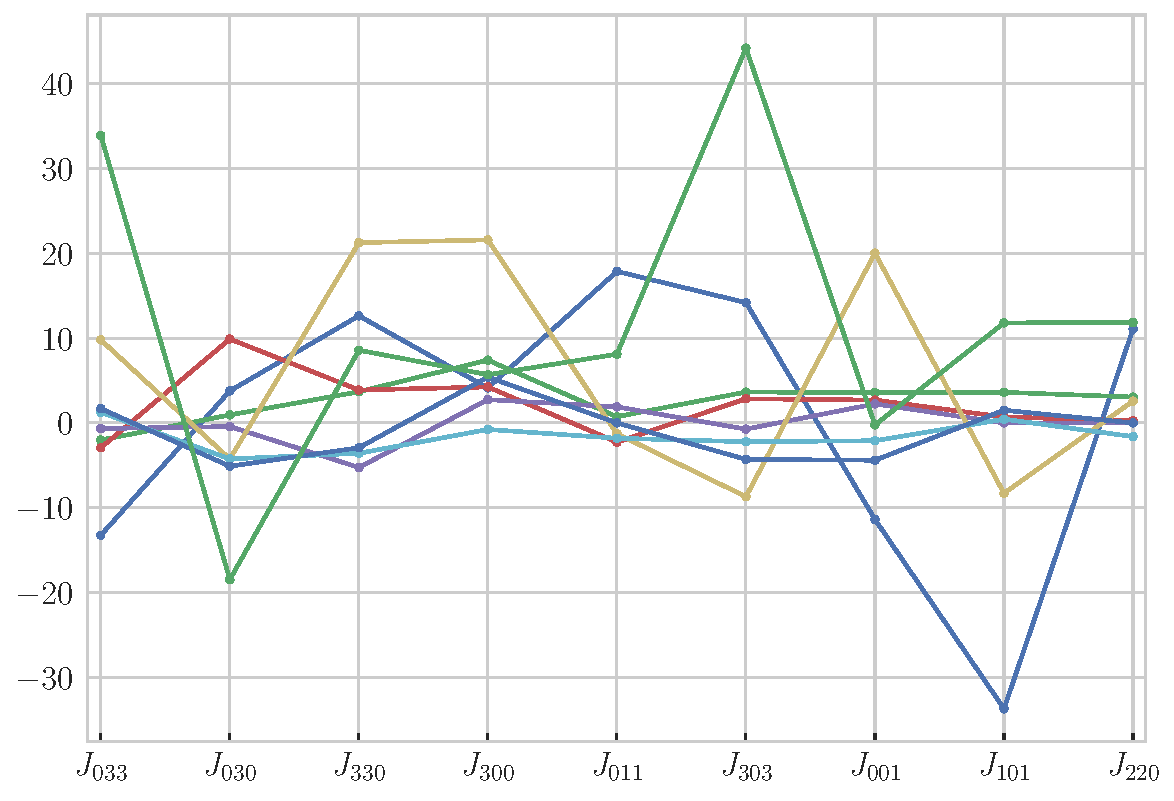
\includegraphics[width=0.5\textwidth]{toffoli_diagonal_solutions}\\
%     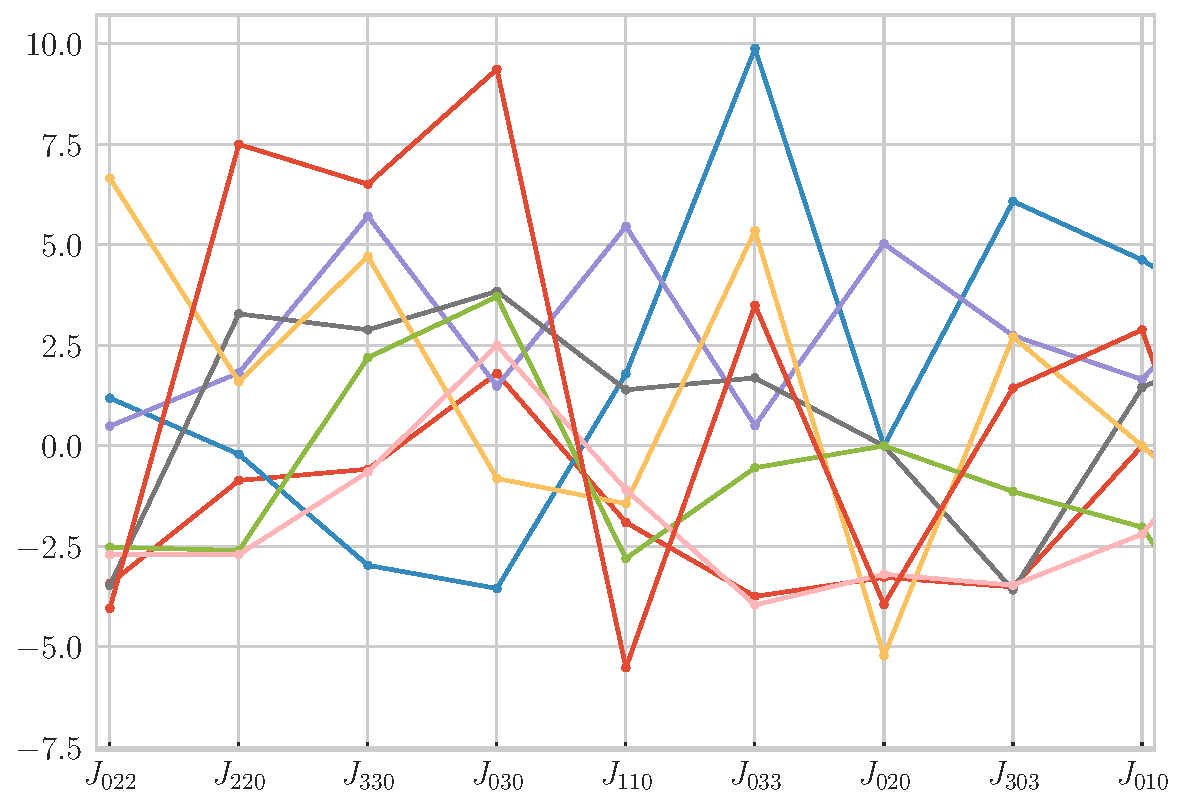
\includegraphics[width=0.5\textwidth]{fredkin_diagonal_solutions}\\
%     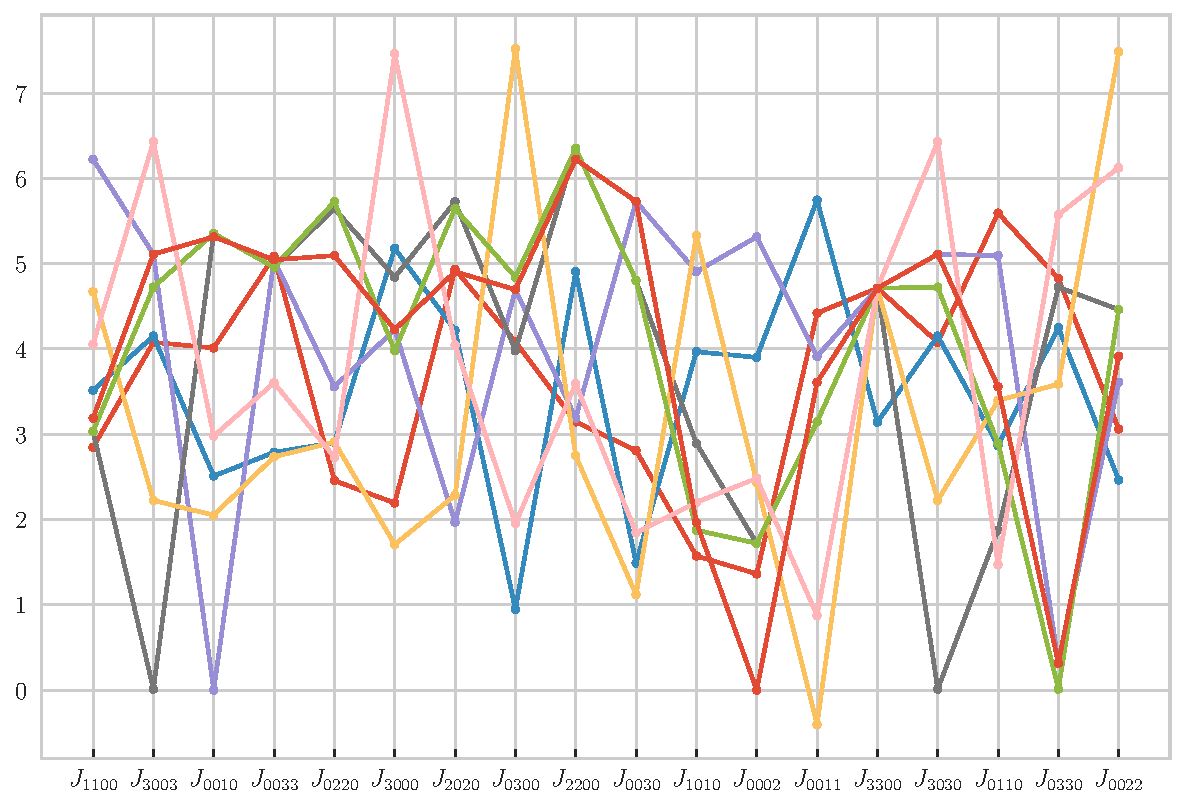
\includegraphics[width=0.5\textwidth]{doublefredkin_diagonal_initvalues4_8samples}
%     \caption{
%         Eight different sets of interaction parameters generating Toffoli [panel {\bf (a)}] and Fredkin [panel {\bf (b)}] gates. For each solution shown here the training was started from the ansatz provided in~\cref{eq:GL:toffoli_reducd_ansatz_for_ML}, and the analogous equation for the Fredkin, respectively. Panel {\bf (c)}: Eight sets of interaction parameters for the ``double Fredkin" gate.
%         Each one of the shown solutions corresponds to unit fidelity up to numerical precision (that is, fidelities greater than $1-10^{-16}$).
%         We refer to the Supplementary Materials for the details of the optimisations.
%     }
%     \label{fig:GL:toffoli_diagonal_solutions}
% \end{figure}

\begin{figure}[tb]
    \vspace{-50pt}
    \begin{subfigure}{\textwidth}
        \centering
        \caption{}
        \label{fig:GL:toffoli_diagonal_solutions}
        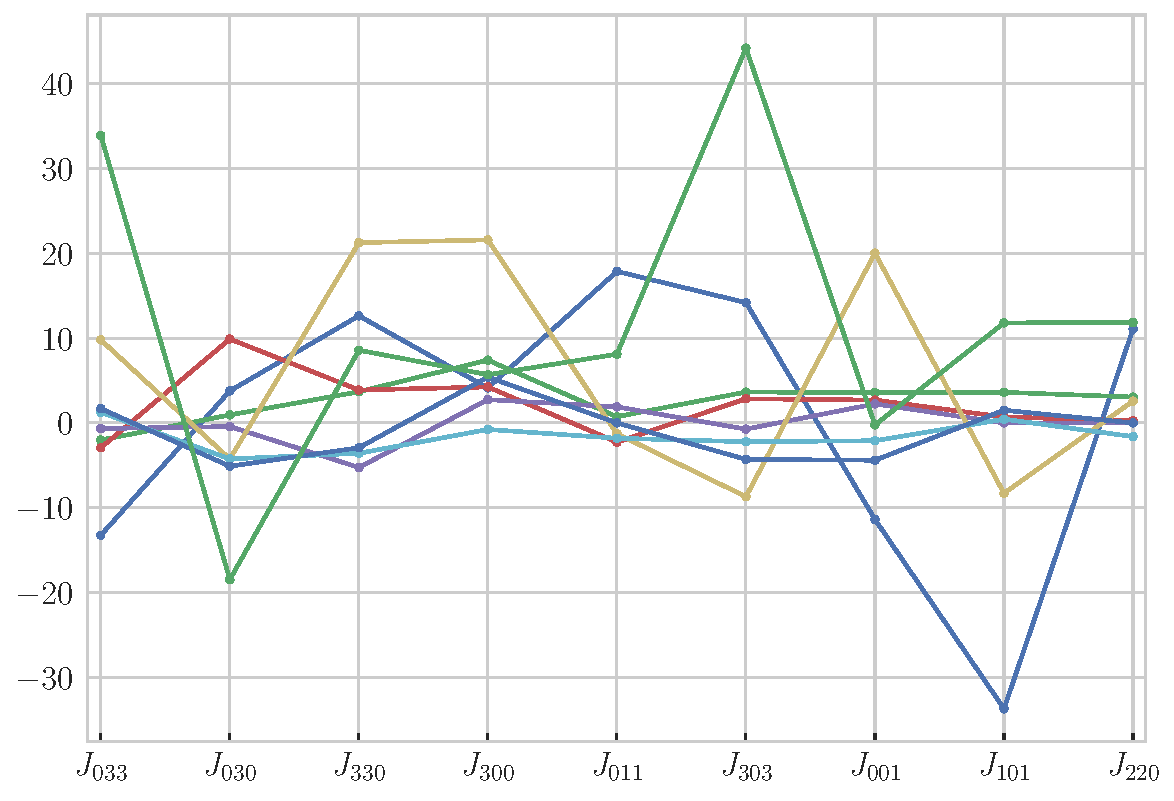
\includegraphics[width=0.5\textwidth]{toffoli_diagonal_solutions}
    \end{subfigure} \\
    \begin{subfigure}{\textwidth}
        \centering
        \caption{}
        \label{fig:GL:fredkin_diagonal_solutions}
        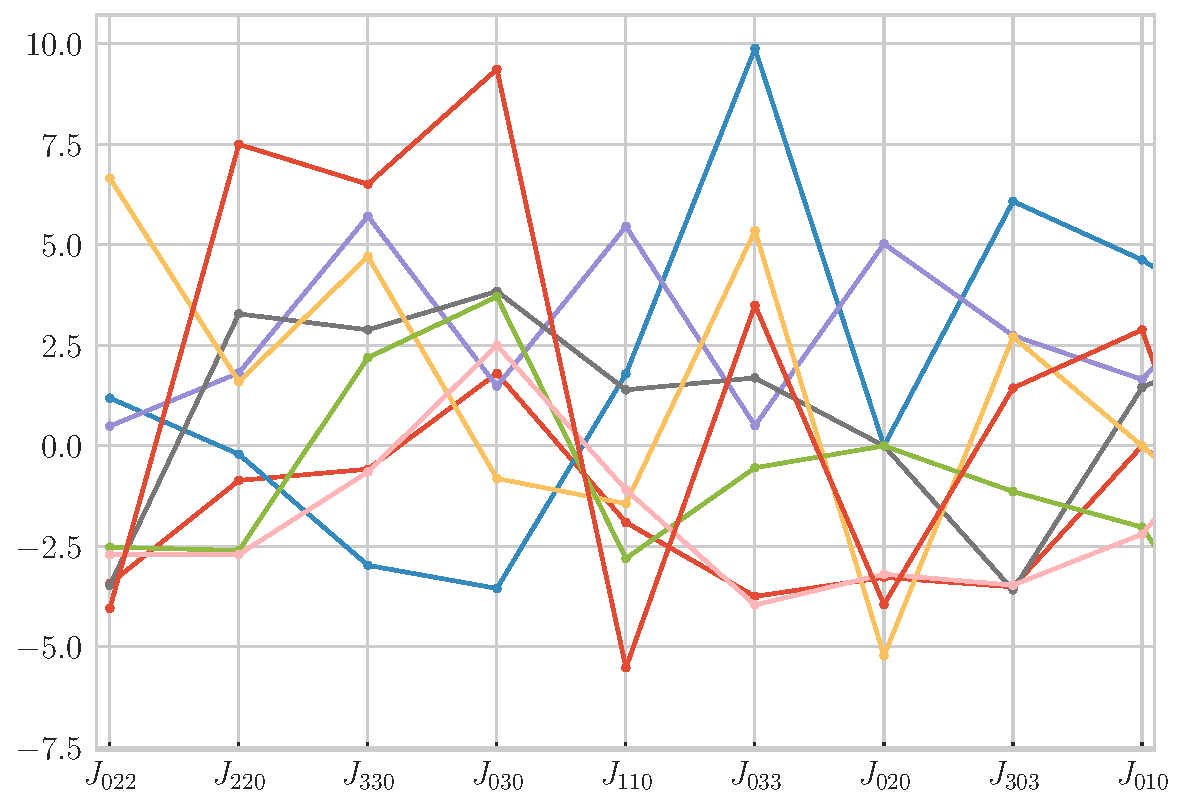
\includegraphics[width=0.5\textwidth]{fredkin_diagonal_solutions}
    \end{subfigure} \\
    \begin{subfigure}{\textwidth}
        \centering
        \caption{}
        \label{fig:GL:doublefredkin_diagonal_solutions}
        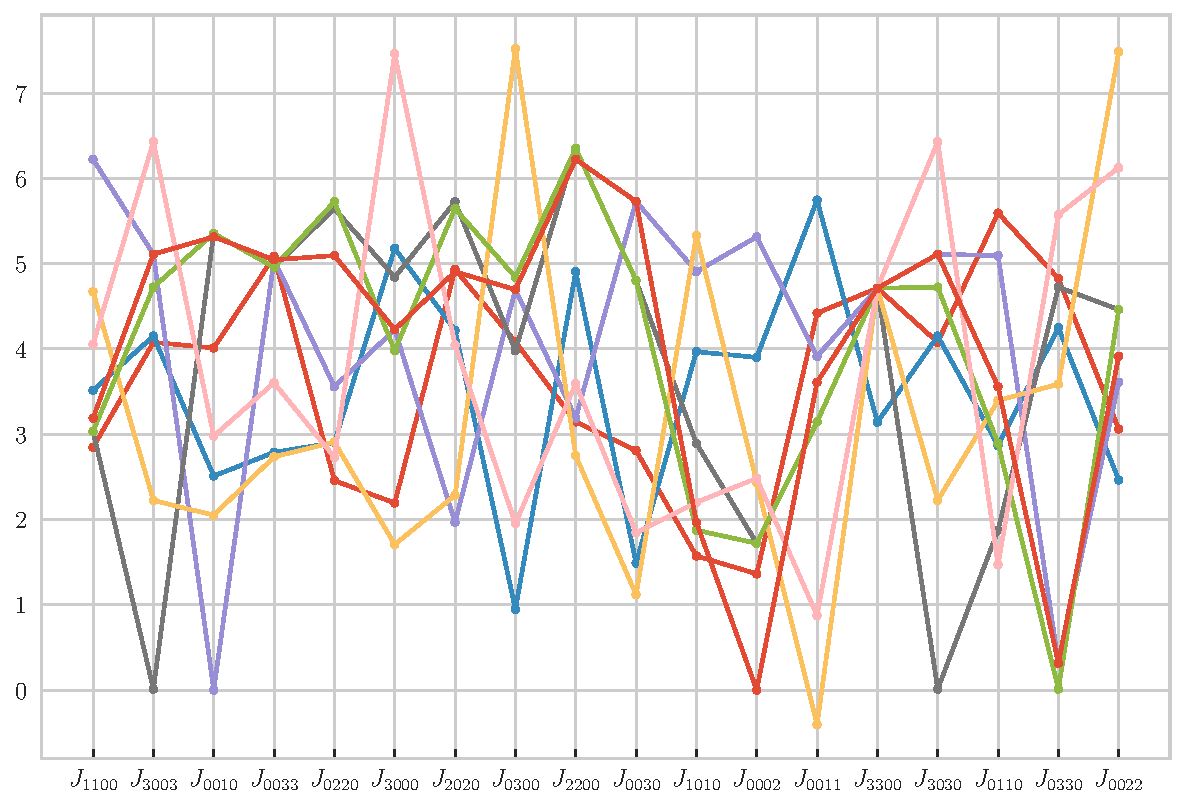
\includegraphics[width=0.5\textwidth]{doublefredkin_diagonal_initvalues4_8samples}
    \end{subfigure}
    \caption{
        Eight different sets of interaction parameters generating Toffoli [panel \textbf{(a)}], Fredkin [panel \textbf{(b)}], and double Fredkin [panel \textbf{(c)}] gates. For each solution shown here the training was started from the ansatz provided in~\cref{eq:GL:toffoli_reducd_ansatz_for_ML}, and the analogous equations for Fredkin and double Fredkin gates.
        Each one of the solutions corresponds to unit fidelity, up to numerical precision (that is, fidelities greater than $1-10^{-16}$).
    }
    \label{fig:GL:toffoli_diagonal_solutions}
\end{figure}

\begin{figure}[tb]
	\centering
	\begin{tikzpicture}
		\node[anchor=south west] (A) at (0, 0)%
			{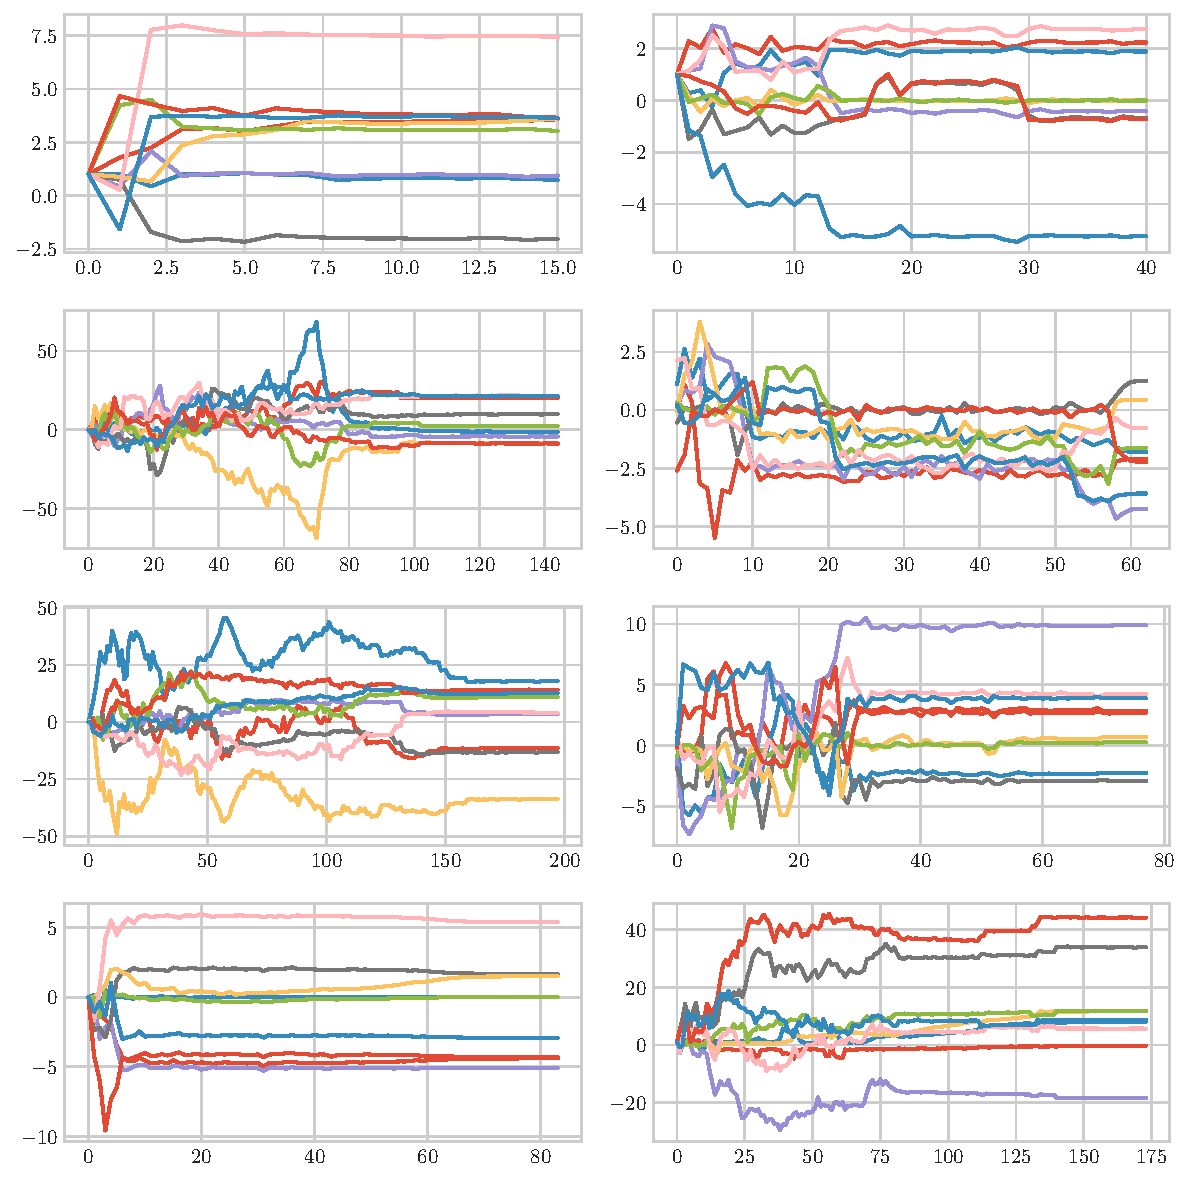
\includegraphics[width=.8\linewidth]{toffoli_diagonal_parhistories}};
		\node[above] at (4., -.2) {$t_e$};
		\node[above] at (11.5, -.2) {$t_e$};
	\end{tikzpicture}%
	% 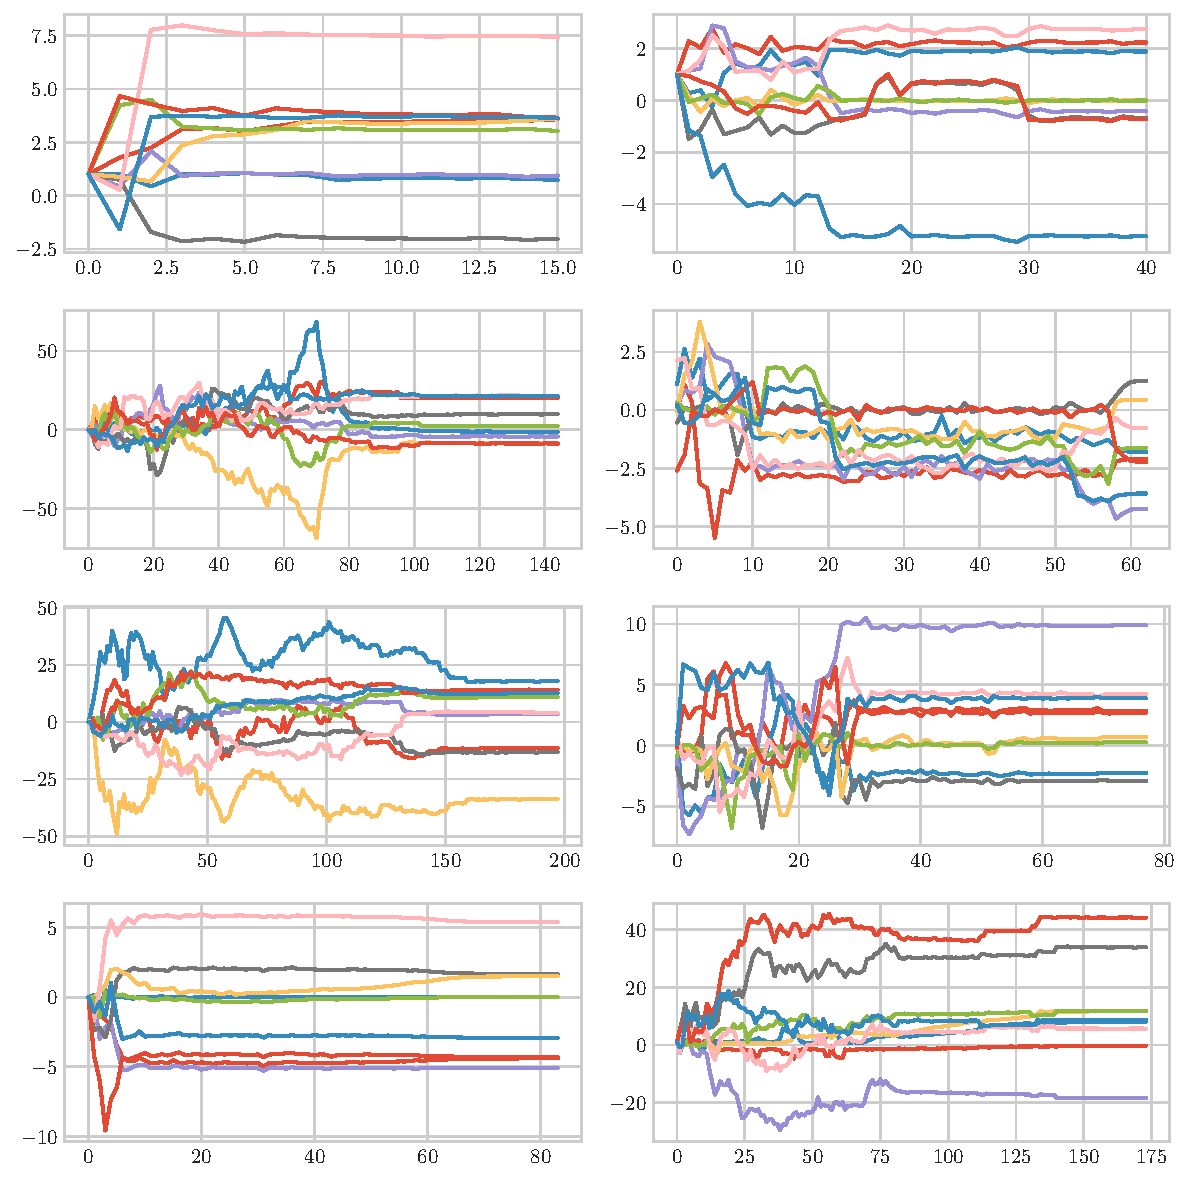
\includegraphics[width=.8\linewidth]{toffoli_diagonal_parhistories}
	\caption{
		Training histories for the \emph{Toffoli} gate with only diagonal interactions.
		In each plot are reported the values of the $9$ network parameters during the training process, for each training epoch $t_e$.
		Each training process was left running until convergence to unit fidelity, therefore, the number of epochs in the horizontal axes differs for different trainings instances.
		The histories shown here correspond to training instances in which the parameters were initialised at various values, as seen from the leftmost values in each plot.
	}
	\label{fig:GL:toffoli_diagonal_parhistories}
\end{figure}
 
% \begin{figure}[tb]
% 	\centering
% 		\begin{tikzpicture}
% 		\node[anchor=south west] (A) at (0, 0)%
% 			{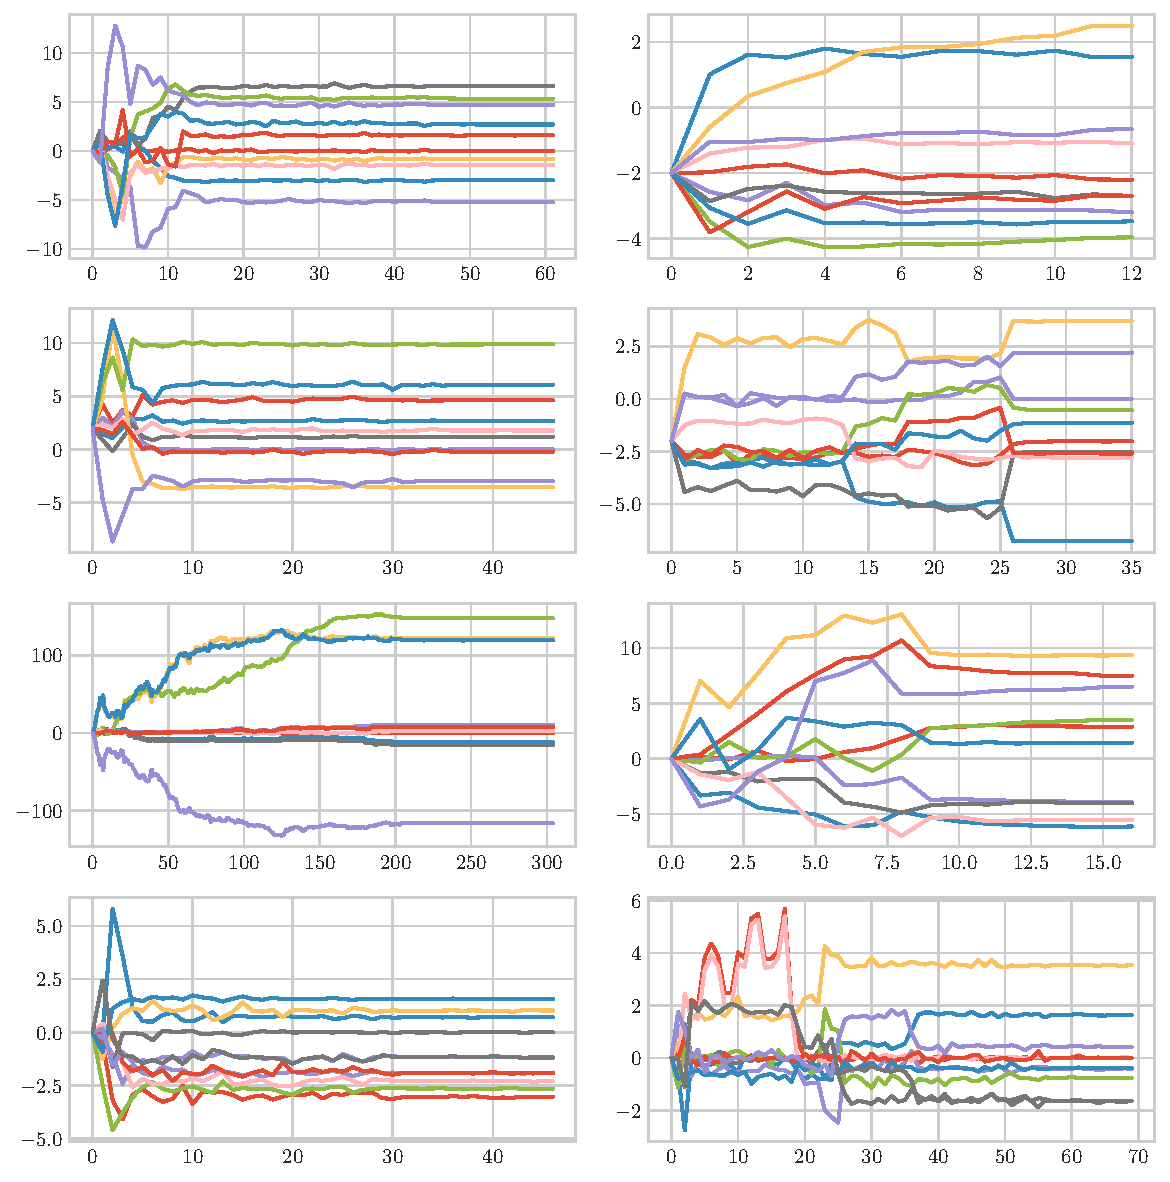
\includegraphics[width=.8\linewidth]{fredkin_diagonal_parhistories}};
% 		\node[above] at (4., -.2) {$t_e$};
% 		\node[above] at (11.5, -.2) {$t_e$};
% 	\end{tikzpicture}%
% 	% 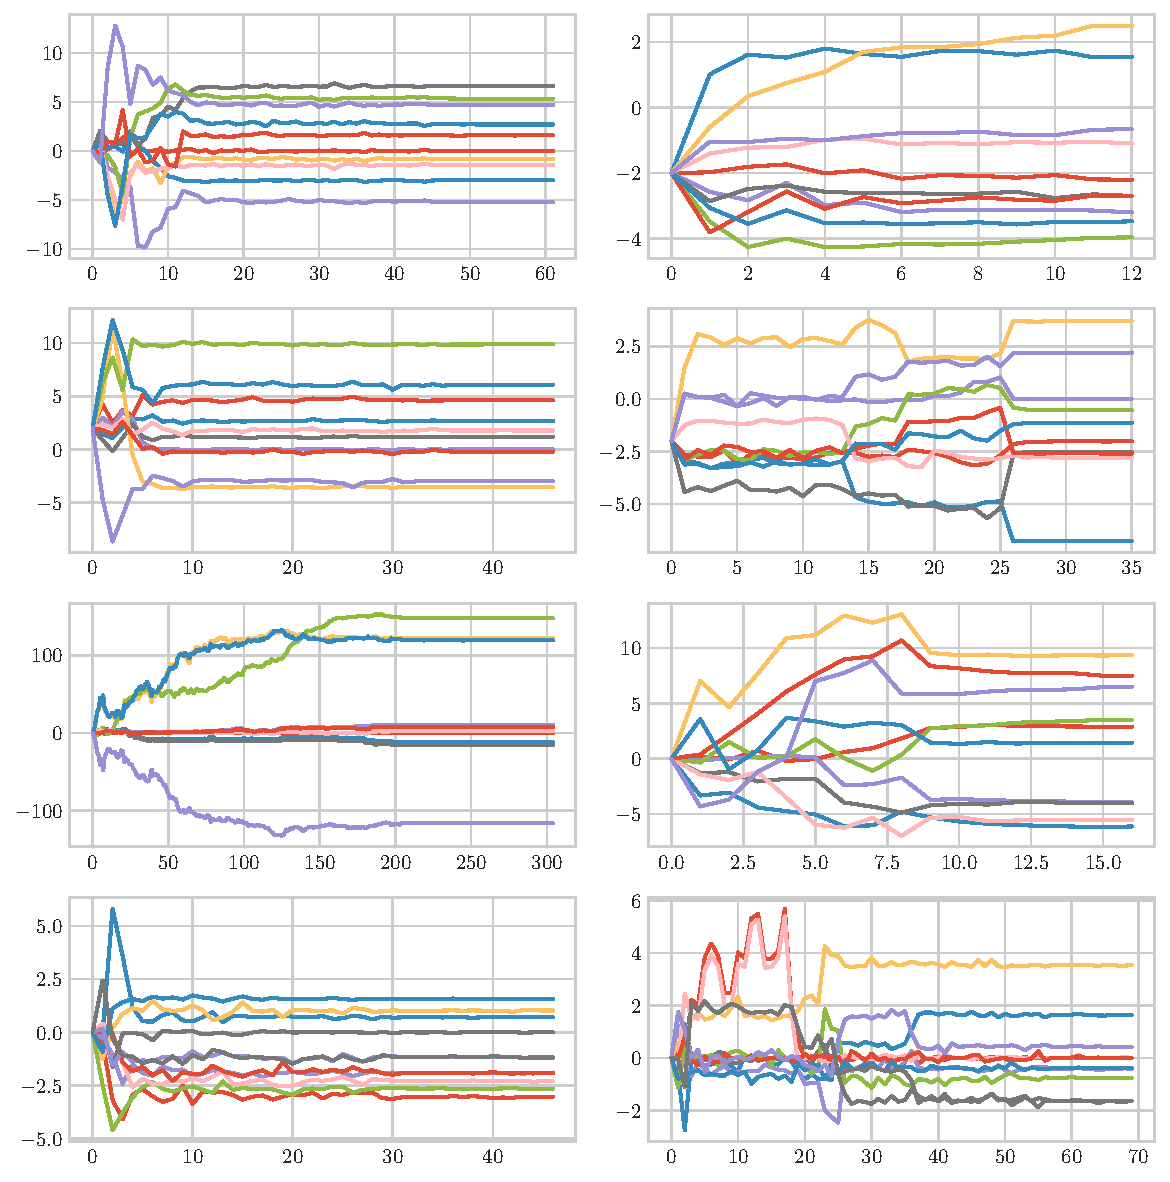
\includegraphics[width=.8\linewidth]{fredkin_diagonal_parhistories}
% 	\caption{
% 		Training histories for the \textbf{Fredkin} gate with only diagonal interactions.
% 		In each plot are reported the values of the $9$ network parameters during the training process, for each training epoch $t_e$.
% 		Each training process was left running until convergence to unit fidelity, therefore, the number of epochs in the horizontal axes differs for different trainings instances.
% 		The histories shown here correspond to training instances in which the parameters were initialised at various values, as seen from the leftmost values in each plot.
% 	}
% 	\label{fig:GL:fredkin_diagonal_parhistories}
% \end{figure}

% \begin{figure}[tb]
% 	\centering
% 	\begin{tikzpicture}
% 		\node[anchor=south west] (A) at (0, 0)%
% 			{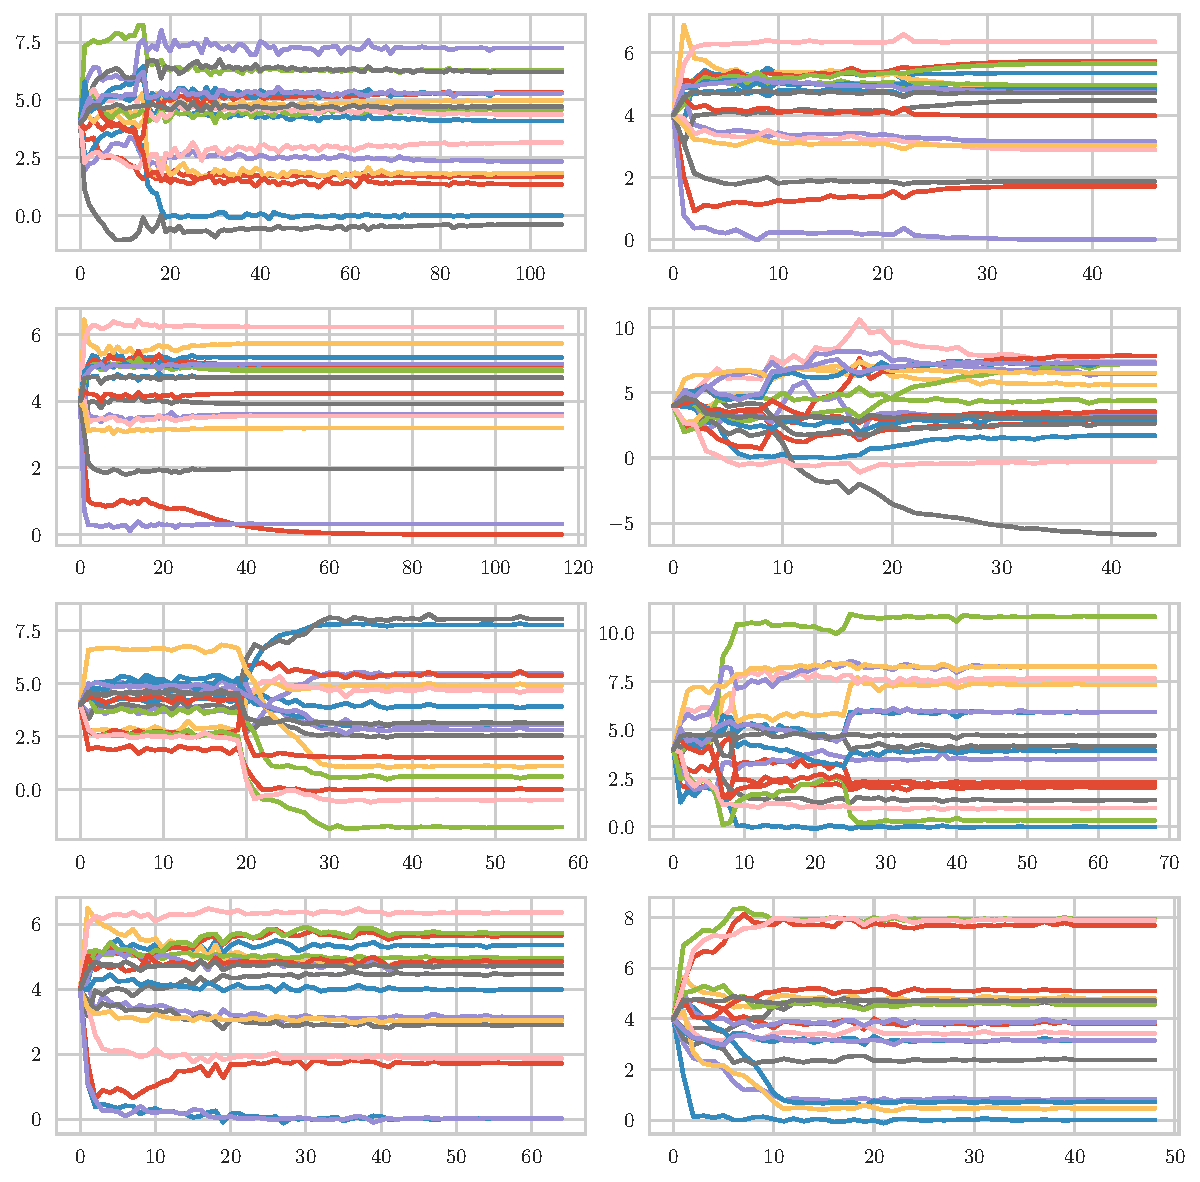
\includegraphics[width=.8\linewidth]{doublefredkin_diagonal_initvalues4_parhistories}};
% 		\node[above] at (4., -.2) {$t_e$};
% 		\node[above] at (11.5, -.2) {$t_e$};
% 	\end{tikzpicture}%
% 	% 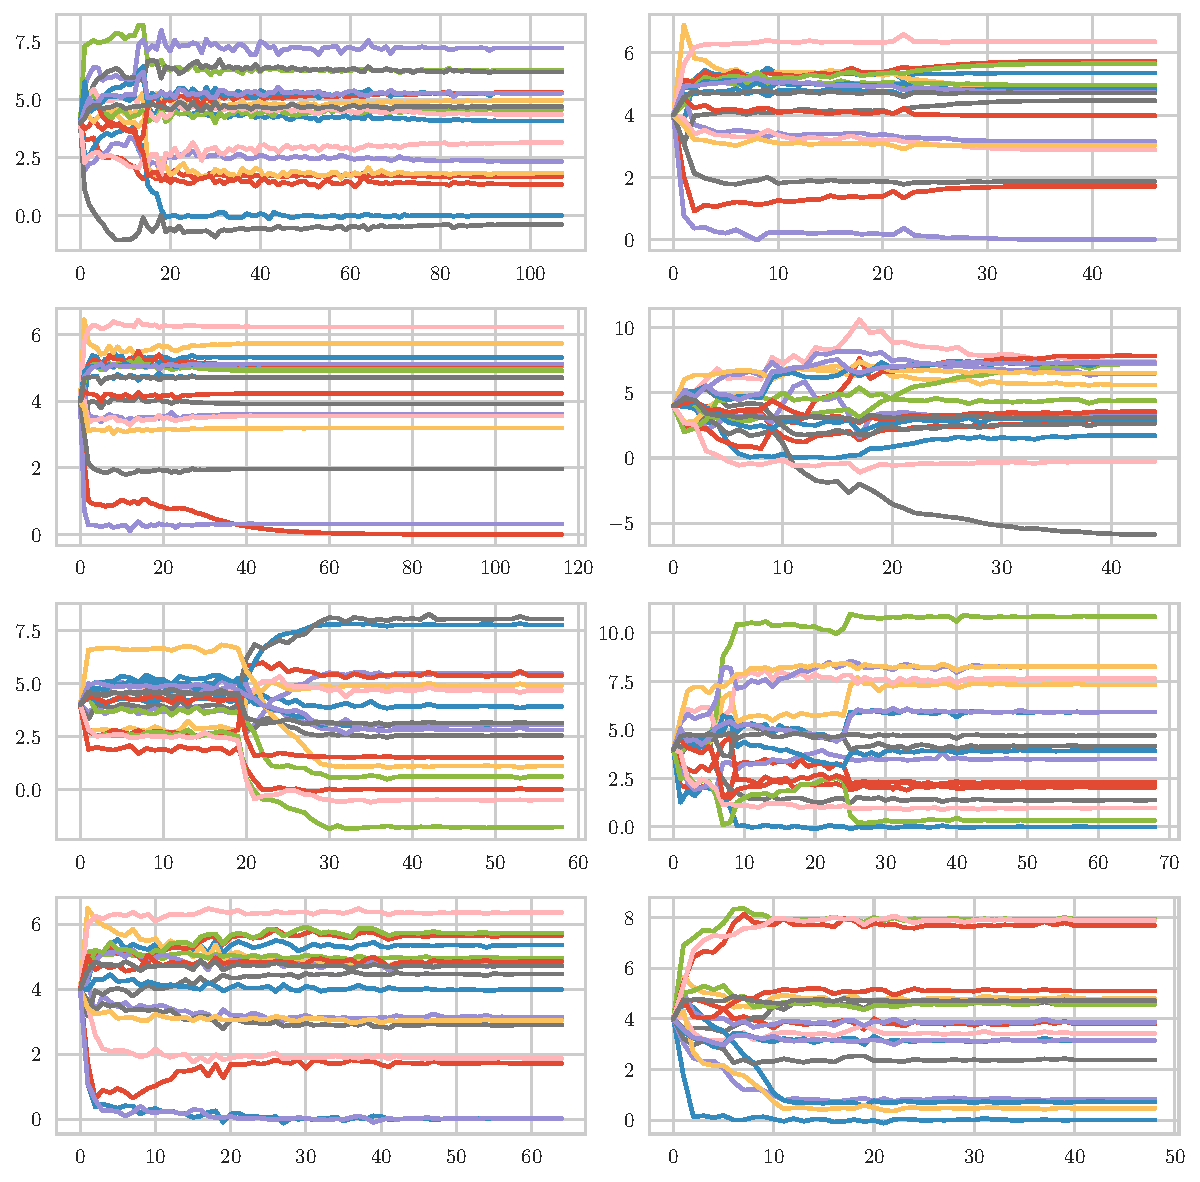
\includegraphics[width=.8\linewidth]{doublefredkin_diagonal_initvalues4_parhistories}
% 	\caption{
% 		Training histories for the \textbf{double-Fredkin} gate with only diagonal interactions.
% 		In each plot are reported the values of the $18$ network parameters during the training process, for each training epoch $t_e$.
% 		Each training process was left running until convergence to unit fidelity, therefore, the number of epochs in the horizontal axes differs for different trainings instances.
% 		All the histories shown here correspond to training instances in which the parameters were initialised to $4$.
% 	}
% 	\label{fig:GL:doublefredkin_diagonal_parhistories}
% \end{figure}

\newcommand{\graphicswithlabel}[3]{%
	\begin{tikzpicture}
		\node[anchor=north west] (A) at (0, 0)%
			{\includegraphics[width=.48\linewidth]{#2}};
		\node[above] at (1.4, -.85) {\small\textbf{(#1)}};
		\node[above] at (4.6, -4.65) {#3};
		\node[above] at (1., -.2) {$\calF_\bslambda(\psi)$};
	\end{tikzpicture}%
}
\begin{figure}[tb]
	\centering
	\graphicswithlabel{a}{toffoli_fidVStime}{$\alpha$}%\vspace{-6pt}
	\graphicswithlabel{b}{toffoli_fidVStime_wide}{$\alpha$}
	\graphicswithlabel{c}{toffoli_fidVSpar0}{$\lambda_1$}\vspace{-6pt}
	\graphicswithlabel{d}{toffoli_fidVSpar1}{$\lambda_2$}
 	\caption{
 		Fidelity $\calF_\bslambda(\psi)$ vs variations of $\bslambda$, for different test states, for the \textbf{Toffoli} gate. The five test states $\psi$ are sampled randomly.
 		\textbf{(a)} Global relative variations of $\bslambda$, that is, plotting the fidelity against $\alpha\bslambda$ for $0.9 \le\alpha\le 1.1$.
 		Note that this is equivalent to studying how the fidelity changes with respect to uncertainties in the evolution time, that is, how much does $\exp(i\calH t')$ differ from $\exp(i\calH t)$.
 		\textbf{(b)} Same as \emph{(a)} but with $0\le\alpha\le 1.2$.
 		\textbf{(c)} Plot of $\calF_\bslambda(\psi)$ against \emph{absolute} variations of a single element of $\bslambda$, in this case the first one, i.e. we take $\lambda_1\in[-10,10]$.
 		\textbf{(d)} Like \emph{(c)} but for $\lambda_2$.
 	}
    \label{fig:toffoli_fidVSpars}
\end{figure}

\renewcommand{\graphicswithlabel}[3]{%
	\begin{tikzpicture}
		\node[anchor=north west] (A) at (0, 0)%
			{\includegraphics[width=.48\linewidth]{#2}};
		\node[above] at (1.4, -.85) {\small\textbf{(#1)}};
		\node[above] at (4.6, -4.65) {#3};
		\node[above] at (1., -.2) {$\calF_\bslambda(\psi)$};
	\end{tikzpicture}%
}
\begin{figure}[tb]
	\centering
	\graphicswithlabel{a}{fredkin_fidVStime}{$\alpha$}\vspace{-6pt}
	\graphicswithlabel{b}{fredkin_fidVStime_wide}{$\alpha$}
	\graphicswithlabel{c}{fredkin_fidVSpar0}{$\lambda_1$}\vspace{-6pt}
	\graphicswithlabel{d}{fredkin_fidVSpar3}{$\lambda_2$}
	\caption{
		Fidelity $\calF_\bslambda(\psi)$ vs variations of $\bslambda$, for different test states, for the \textbf{Fredkin} gate. The five test states $\psi$ are sampled randomly.
		\textbf{(a)} Global relative variations of $\bslambda$, that is, plotting the fidelity against $\alpha\bslambda$ for $0.9 \le\alpha\le 1.1$.
		Note that this is equivalent to studying how the fidelity changes with respect to uncertainties in the evolution time, that is, how much does $\exp(i\calH t')$ differ from $\exp(i\calH t)$.
		\textbf{(b)} Same as \emph{(a)} but with $0\le\alpha\le 1.2$.
		\textbf{(c)} Plot of $\calF_\bslambda(\psi)$ against \emph{absolute} variations of a single element of $\bslambda$, in this case the first one, i.e. we take $\lambda_1\in[-10,10]$.
		\textbf{(d)} Like \emph{(c)} but for $\lambda_2$.
	}
	\label{fig:fredkin_fidVSpars}
\end{figure}

\renewcommand{\graphicswithlabel}[3]{%
	\begin{tikzpicture}
		\node[anchor=north west] (A) at (0, 0)%
			{\includegraphics[width=.48\linewidth]{#2}};
		\node[above] at (1.4, -.85) {\small\textbf{(#1)}};
		\node[above] at (4.6, -4.65) {#3};
		\node[above] at (1., -.2) {$\calF_\bslambda(\psi)$};
	\end{tikzpicture}%
}
\begin{figure}[tb]
	\centering
	\graphicswithlabel{a}{doublefredkin_fidVStime}{$\alpha$}\vspace{-6pt}
	\graphicswithlabel{b}{doublefredkin_fidVStime_wide}{$\alpha$}
	\graphicswithlabel{c}{doublefredkin_fidVSpar0}{$\lambda_1$}\vspace{-6pt}
	\graphicswithlabel{d}{doublefredkin_fidVSpar1}{$\lambda_2$}
	\caption{
		Fidelity $\calF_\bslambda(\psi)$ vs variations of $\bslambda$, for different test states, for the \textbf{double Fredkin} gate. The five test states $\psi$ are sampled randomly.
		\textbf{(a)} Global relative variations of $\bslambda$, that is, plotting the fidelity against $\alpha\bslambda$ for $0.9 \le\alpha\le 1.1$.
		Note that this is equivalent to studying how the fidelity changes with respect to uncertainties in the evolution time, that is, how much does $\exp(i\calH t')$ differ from $\exp(i\calH t)$.
		\textbf{(b)} Same as \emph{(a)} but with $0\le\alpha\le 1.2$.
		\textbf{(c)} Plot of $\calF_\bslambda(\psi)$ against \emph{absolute} variations of a single element of $\bslambda$, in this case the first one, i.e. we take $\lambda_1\in[-10,10]$.
		\textbf{(d)} Like \emph{(c)} but for $\lambda_2$.
	}
	\label{fig:doublefredkin_fidVSpars}
\end{figure}


\newcommand{\traininggraphicswithlabel}[1]{%
	\begin{tikzpicture}
		\node[anchor=north west] (A) at (0, 0)%
			{\includegraphics[width=.85\linewidth]{#1}};
		\node[above] at (0, -.8) {$\barcalF$};
	\end{tikzpicture}%
}

\begin{figure}[tb]
	\centering
	% 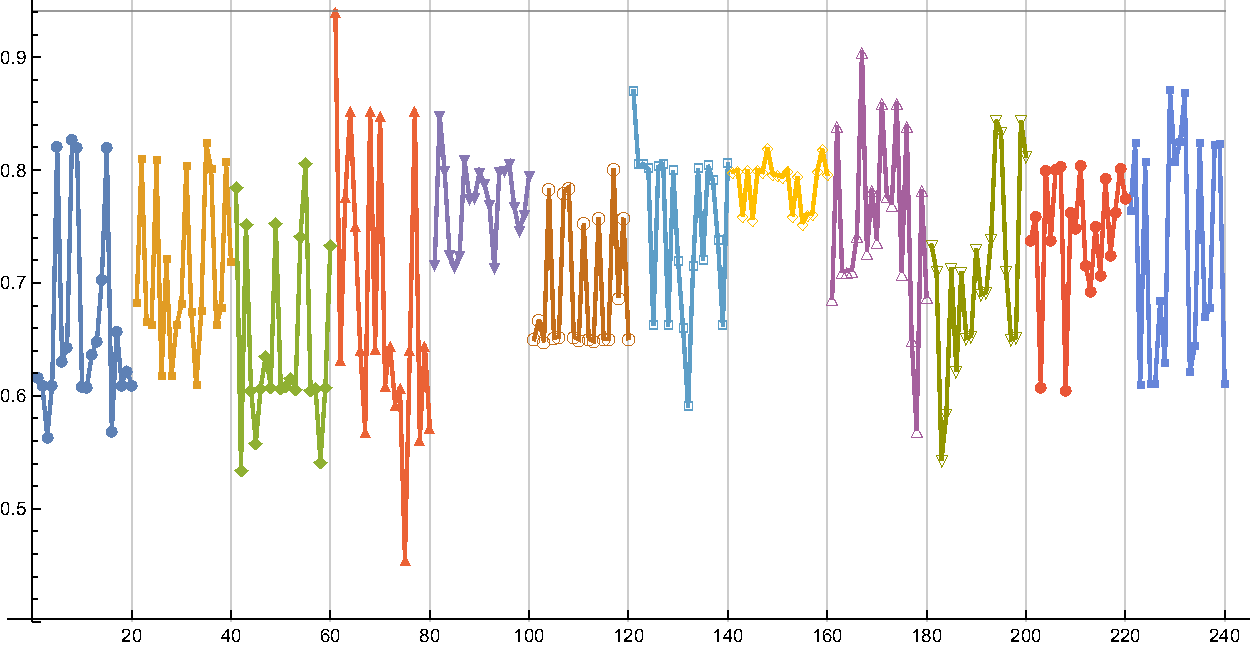
\includegraphics[width=.85\linewidth]{fredkin_noancillae_XXall.pdf}
    \vspace{-40pt}
	\traininggraphicswithlabel{fredkin_noancillae_XXall.pdf}
	\caption{
		Training results for the \textbf{Fredkin} gate with a generator containing one-qubit interactions and two-qubit interactions of the form $J_{ij}(X_i X_j + Y_i Y_j)$.
		Every point shows the final fidelity obtained at the end of a training procedure.
		The hyperparameters, as well as the total number of training iterations, are kept the same in all the training instances shown here.
		The initial parameters' values are the same within each horizontal sector, but changed between different sectors.
		The initial parameters' values within each sector have been chosen as all equal to $c$ (that is, $\lambda_i=c$ for all $i$). The values of $c$ are $0, 1,\ldots, 10$, with $c=0$ in the leftmost sector and $c=10$ in the last to rightmost one.
		The rightmost sector contains the results of training attempts with the initial values chosen at random (that is, with $\lambda_i$ sampled according to the uniform normal distribution, independently for each $i$).
		The greatest reached fidelity, obtained with initial parameters' values $\lambda_i=3$, is $\calF\simeq0.94$.
	}
\label{fig:fredkin_XX}
\end{figure}

\begin{figure}[tb]
	\centering
	\traininggraphicswithlabel{fredkin_noancillae_XYall.pdf}
	\caption{
		Training results for the \textbf{Fredkin} gate with a generator containing all one-qubit interactions and two-qubit interactions of the form $J^{(1)}_{ij}X_i X_j + J^{(2)}_{ij}Y_i Y_j$.
		The initial conditions are chosen as in~\cref{fig:fredkin_XX}.
		The maximum fidelities obtained are $\calF\simeq0.999$, obtained in multiple instances $c=3$ and $c=4$ sectors.
	}
\label{fig:fredkin_XY}
\end{figure}

\begin{figure}[tb]
	\centering
	\traininggraphicswithlabel{toffoli_noancillae_XXall.pdf}
	\caption{
		Training results for the \textbf{Toffoli} gate with a generator containing all one-qubit interactions and two-qubit interactions of the form $J_{ij}(X_i X_j + Y_i Y_j)$.
		The initial conditions are chosen as in~\cref{fig:fredkin_XX}.
		The maximum fidelities obtained are $\calF\simeq0.94$, obtained in the $c=3$ sector.
	}
	\label{fig:toffoli_XX}
\end{figure}

\begin{figure}[tb]
	\centering
	\traininggraphicswithlabel{toffoli_noancillae_XYall.pdf}
	\caption{
		Training results for the \textbf{Toffoli} gate with a generator containing all one-qubit interactions and two-qubit interactions of the form $J^{(1)}_{ij}X_i X_j + J^{(2)}_{ij}Y_i Y_j$.
		The initial conditions are chosen as in~\cref{fig:fredkin_XX}.
		The maximum fidelities obtained are $\calF\simeq0.98$, obtained in the $c=4$ and $c=5$ sectors.
	}
	\label{fig:toffoli_XY}
\end{figure}


\renewcommand{\graphicswithlabel}[2]{%
    \begin{tikzpicture}
        \node[anchor=south west, inner sep=0] at (0, 0)%
            {\includegraphics[width=.8\linewidth]{#2}};
        \node[above] at (1, 4.6) {\textbf{(#1)}};
    \end{tikzpicture}%
}
\begin{figure}
    \centering
    \vspace{-40pt}%
    \graphicswithlabel{a}{verona-qft3q+5a_all}
    \graphicswithlabel{b}{verona-toffredkin_all}
    \graphicswithlabel{c}{verona-halfadder_all}
    \caption{
        Trained parameters for the three-qubit \ac{QFT}, Toffredkin and half-adder networks. We plot the values taken by the elements of the full set of parameters entering Eq. (6) and ordered as ${\bslambda}=\{h_0,h^1_1,\dots,h^3_N,J^{11}_{11},\dots,J^{33}_{NN}\}$ with $N$ the number of elements of the qubit network.
    }
    \label{fig:GL:parameters_QFT_Toffredkin_halfadder}
\end{figure}

\renewcommand{\graphicswithlabel}[3]{%
    \begin{tikzpicture}
        \node[anchor=north west] (A) at (0, 0)%
            {\includegraphics[width=.6\linewidth]{#2}};
        \node[above] at (1.5, -.85) {\small\textbf{(#1)}};
        \node[above] at (4.3, -4.4) {#3};
        \node[above] at (1.1, -.3) {$\mathcal F_\bslambda(\psi)$};
    \end{tikzpicture}%
}
\begin{figure}
    \centering
    % \vspace{-40pt}%
    \graphicswithlabel{a}{verona-toffredkin_fidVStime}{$\alpha$}\vspace{-6pt}
    \graphicswithlabel{b}{verona-toffredkin_fidVStime_wide}{$\alpha$}\vspace{-6pt}
    \graphicswithlabel{c}{verona-toffredkin_fidVSpar0}{$\lambda_1$}\vspace{-6pt}
    \caption{\footnotesize
        Fidelity $\calF_\bslambda(\psi)$ vs variations of $\bslambda$, for different test states, for the \textbf{Toffredkin} gate. The five test states $\psi$ are sampled randomly.
        \textbf{(a)} Global relative variations of $\bslambda$, that is, plotting the fidelity against $\alpha\bslambda$ for $0.9 \le\alpha\le 1.1$.
        Note that this is equivalent to studying how the fidelity changes with respect to uncertainties in the evolution time, that is, how much does $\exp(i\calH t')$ differ from $\exp(i\calH t)$.
        \textbf{(b)} Same as \emph{(a)} but with $0\le\alpha\le 1.2$.
        \textbf{(c)} Plot of $\calF_\bslambda(\psi)$ against \emph{absolute} variations of a single element of $\bslambda$, in this case the first one, i.e. we take $\lambda_1\in[-10,10]$.
        \textbf{(d)} Like \emph{(c)} but for $\lambda_2$.
    }
    \label{fig:GL:toffredkin_fidVSpars}
\end{figure}

\begin{figure}
    \centering
    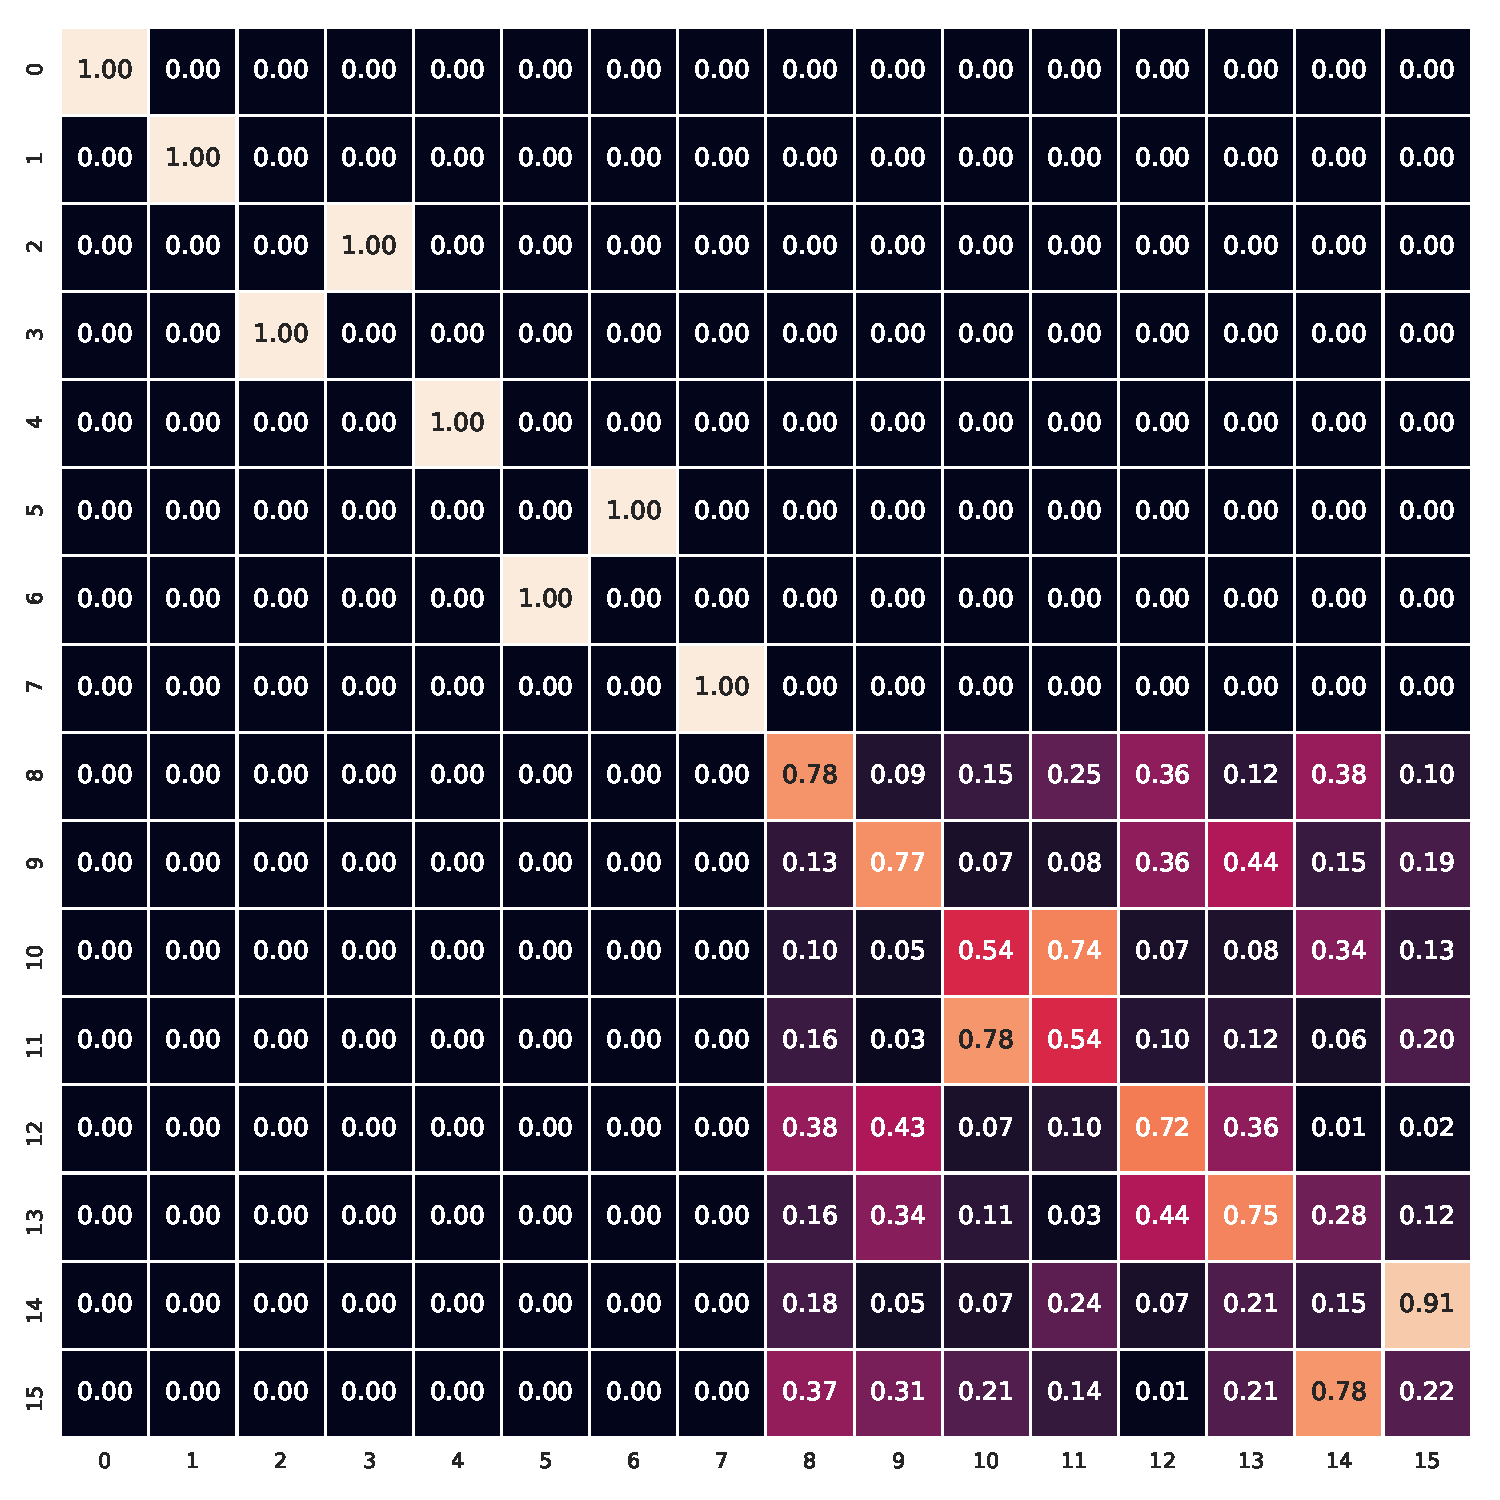
\includegraphics[width=\linewidth]{verona-toffredkin_finalmatrix}
    \caption{
        Final \textbf{Toffredkin} gate found from the supervised learning training.
        In this representation, the ancillary qubit is the first one, so that the top-left $8\times8$ submatrix describes the evolution of states when the ancillary qubit starts as $\ket0$.
        Notably, it is clear from the matrix that the gate acts diagonally on the ancillary qubits, which therefore effectively acts as a control qubit.
        When this control ancillary qubit is $\ket0$, the other three qubits evolve according to the Toffredkin gate.
    }
    \label{fig:GL:toffredkin_finalmatrix}
\end{figure}

\renewcommand{\graphicswithlabel}[3]{%
    \begin{tikzpicture}
        \node[anchor=north west] (A) at (0, 0)%
            {\includegraphics[width=.6\linewidth]{#2}};
        \node[above] at (1, -.85) {\small\textbf{(#1)}};
        \node[above] at (4.3, -4.4) {#3};
        \node[above] at (1.1, -.3) {$\mathcal F_\bslambda(\psi)$};
    \end{tikzpicture}%
}
\begin{figure}
    \centering
    % \vspace{-40pt}
    \graphicswithlabel{a}{verona-qft3q+5a_fidVStime}{$\alpha$}\vspace{-6pt}
    \graphicswithlabel{b}{verona-qft3q+5a_fidVStime_wide}{$\alpha$}\vspace{-6pt}
    \graphicswithlabel{c}{verona-qft3q+5a_fidVSpar0}{$\lambda_1$}\vspace{-6pt}
    % \graphicswithlabel{d}{verona-qft3q+5a_fidVSpar1}{$\lambda_2$}\vspace{-6pt}
    \caption{
        Fidelity $\calF_\bslambda(\psi)$ vs variations of $\bslambda$, for different test states, for the \textbf{three-qubit QFT} gate. The five test states $\psi$ are sampled randomly.
        \textbf{(a)} Global relative variations of $\bslambda$, that is, plotting the fidelity against $\alpha\bslambda$ for $0.9 \le\alpha\le 1.1$.
        Note that this is equivalent to studying how the fidelity changes with respect to uncertainties in the evolution time, that is, how much does $\exp(i\calH t')$ differ from $\exp(i\calH t)$.
        \textbf{(b)} Same as \emph{(a)} but with $0\le\alpha\le 1.2$.
        \textbf{(c)} Plot of $\calF_\bslambda(\psi)$ against \emph{absolute} variations of a single element of $\bslambda$, in this case the first one, i.e. we take $\lambda_1\in[-10,10]$.
        % \textbf{(d)} Like \emph{(c)} but for $\lambda_2$.
    }
    \label{fig:GL:qft3q+5a_fidVSpars}
\end{figure}
% \thispagestyle{empty}

\renewcommand{\graphicswithlabel}[3]{%
    \begin{tikzpicture}
        \node[anchor=north west] at (0, 0)%
            {\includegraphics[width=.64\linewidth]{#2}};
        \node[above] at (1, -.85) {\small\textbf{(#1)}};
        \node[above] at (4.3, -4.4) {#3};
        \node[above] at (1.1, -.3) {$\mathcal F_\bslambda(\psi)$};
    \end{tikzpicture}%
}
\begin{figure}
    \centering
    \graphicswithlabel{a}{verona-halfadder_fidVStime}{$\alpha$}\vspace{-6pt}
    \graphicswithlabel{b}{verona-halfadder_fidVStime_wide}{$\alpha$}\vspace{-6pt}
    \graphicswithlabel{c}{verona-halfadder_fidVSpar0}{$\lambda_1$}\vspace{-6pt}
    % \graphicswithlabel{d}{verona-halfadder_fidVSpar1}{$\lambda_2$}
    \caption{
        Fidelity $\calF_\bslambda(\psi)$ vs variations of $\bslambda$, for different test states, for the \textbf{half-adder} gate. The five test states $\psi$ are sampled randomly.
        \textbf{(a)} Global relative variations of $\bslambda$, that is, plotting the fidelity against $\alpha\bslambda$ for $0.9 \le\alpha\le 1.1$.
        Note that this is equivalent to studying how the fidelity changes with respect to uncertainties in the evolution time, that is, how much does $\exp(i\calH t')$ differ from $\exp(i\calH t)$.
        \textbf{(b)} Same as \emph{(a)} but with $0\le\alpha\le 1.2$.
        \textbf{(c)} Plot of $\calF_\bslambda(\psi)$ against \emph{absolute} variations of a single element of $\bslambda$, in this case the first one, i.e. we take $\lambda_1\in[-10,10]$.
        % \textbf{(d)} Like \emph{(c)} but for $\lambda_2$.
    }
    \label{fig:GL:halfadder_fidVSpars}
\end{figure}

\begin{figure}
    \centering
    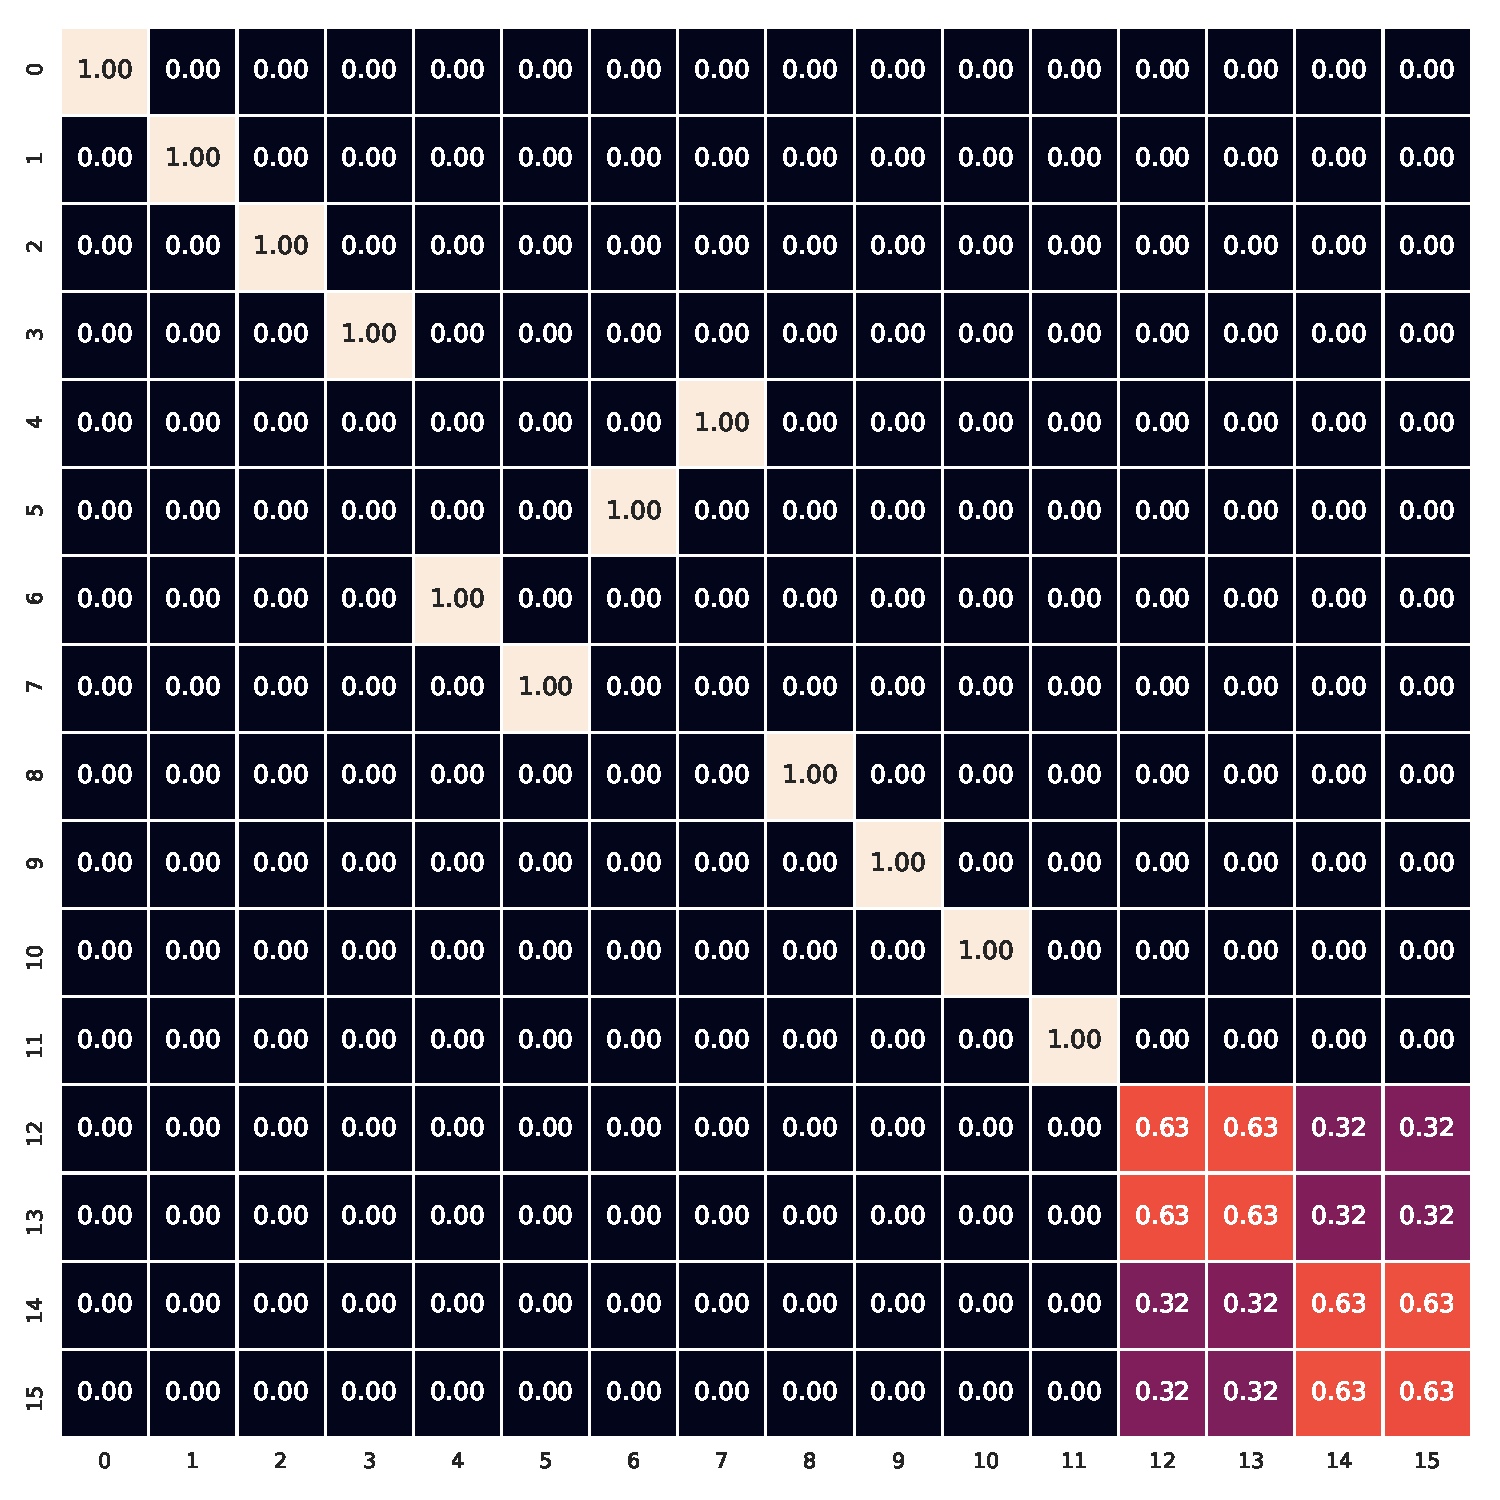
\includegraphics[width=\linewidth]{verona-halfadder_finalmatrix}
    \caption{
        Final \textbf{half-adder} gate found from the supervised learning training.
        In this representation, the ancillary qubit is the first one, so that the top-left $8\times8$ submatrix describes the evolution of states when the ancillary qubit starts as $\ket0$.
        Notably, it is clear from the matrix that the gate acts diagonally on the ancillary qubits, which therefore effectively acts as a control qubit, which when $\ket0$ induces the other three qubits to evolve according to the half-adder gate.
    }
    \label{fig:GL:halfadder_finalmatrix}
\end{figure}
